% **************************************************************************************************************
% A Classic Thesis Style
% An Homage to The Elements of Typographic Style
%
% Copyright (C) 2018 André Miede and Ivo Pletikosić
%
% If you like the style then I would appreciate a postcard. My address
% can be found in the file ClassicThesis.pdf. A collection of the
% postcards I received so far is available online at
% http://postcards.miede.de
%
% License:
% This program is free software; you can redistribute it and/or modify
% it under the terms of the GNU General Public License as published by
% the Free Software Foundation; either version 2 of the License, or
% (at your option) any later version.
%
% This program is distributed in the hope that it will be useful,
% but WITHOUT ANY WARRANTY; without even the implied warranty of
% MERCHANTABILITY or FITNESS FOR A PARTICULAR PURPOSE.  See the
% GNU General Public License for more details.
%
% You should have received a copy of the GNU General Public License
% along with this program; see the file COPYING.  If not, write to
% the Free Software Foundation, Inc., 59 Temple Place - Suite 330,
% Boston, MA 02111-1307, USA.
%
% PLEASE SEE ALSO THE AUTHORS' NOTE REGARDING THIS LICENSE
% IN THE DOCUMENTATION (ClassicThesis.pdf --> Chapter 1 / Chapter01.tex)
% **************************************************************************************************************
\RequirePackage{silence} % :-\
    \WarningFilter{scrreprt}{Usage of package `titlesec'}
    %\WarningFilter{scrreprt}{Activating an ugly workaround}
    \WarningFilter{titlesec}{Non standard sectioning command detected}
\documentclass[ oneside,openright,titlepage,numbers=noenddot,%1headlines,
                headinclude,footinclude,cleardoublepage=empty,abstract=on,
                BCOR=5mm,paper=letter,fontsize=10.5pt
                ]{scrreprt}
\special{dvipdfmx:config z 3}
%********************************************************************
% Note: Make all your adjustments in here
%*******************************************************
% ****************************************************************************************************
% classicthesis-config.tex
% formerly known as loadpackages.sty, classicthesis-ldpkg.sty, and classicthesis-preamble.sty
% Use it at the beginning of your ClassicThesis.tex, or as a LaTeX Preamble
% in your ClassicThesis.{tex,lyx} with % ****************************************************************************************************
% classicthesis-config.tex
% formerly known as loadpackages.sty, classicthesis-ldpkg.sty, and classicthesis-preamble.sty
% Use it at the beginning of your ClassicThesis.tex, or as a LaTeX Preamble
% in your ClassicThesis.{tex,lyx} with % ****************************************************************************************************
% classicthesis-config.tex
% formerly known as loadpackages.sty, classicthesis-ldpkg.sty, and classicthesis-preamble.sty
% Use it at the beginning of your ClassicThesis.tex, or as a LaTeX Preamble
% in your ClassicThesis.{tex,lyx} with \input{classicthesis-config}
% ****************************************************************************************************
% If you like the classicthesis, then I would appreciate a postcard.
% My address can be found in the file ClassicThesis.pdf. A collection
% of the postcards I received so far is available online at
% http://postcards.miede.de
% ****************************************************************************************************


% ****************************************************************************************************
% 0. Set the encoding of your files. UTF-8 is the only sensible encoding nowadays. If you can't read
% äöüßáéçèê∂åëæƒÏ€ then change the encoding setting in your editor, not the line below. If your editor
% does not support utf8 use another editor!
% ****************************************************************************************************
\PassOptionsToPackage{utf8}{inputenc}
\usepackage{inputenc}

\PassOptionsToPackage{T1}{fontenc} % T2A for cyrillics
\usepackage{fontenc}


% ****************************************************************************************************
% 1. Configure classicthesis for your needs here, e.g., remove "drafting" below
% in order to deactivate the time-stamp on the pages
% (see ClassicThesis.pdf for more information):
% ****************************************************************************************************
\PassOptionsToPackage{
  drafting=true,    % print version information on the bottom of the pages
  tocaligned=false, % the left column of the toc will be aligned (no indentation)
  dottedtoc=true,  % page numbers in ToC flushed right
  eulerchapternumbers=true, % use AMS Euler for chapter font (otherwise Palatino)
  linedheaders=false,       % chaper headers will have line above and beneath
  floatperchapter=true,     % numbering per chapter for all floats (i.e., Figure 1.1)
  eulermath=true,  % use awesome Euler fonts for mathematical formulae (only with pdfLaTeX)
  beramono=true,    % toggle a nice monospaced font (w/ bold)
  palatino=false,    % deactivate standard font for loading another one, see the last section at the end of this file for suggestions
  style=classicthesis % classicthesis, arsclassica
}{classicthesis}


% ****************************************************************************************************
% 2. Personal data and user ad-hoc commands (insert your own data here)
% ****************************************************************************************************
\newcommand{\myTitle}{Operating Systems for Far Out Memories\xspace}
\newcommand{\mySubtitle}{Building a new OS for Upcoming Hardware\xspace}
%\newcommand{\myDegree}{Doktor-Ingenieur (Dr.-Ing.)\xspace}
\newcommand{\myName}{Daniel Bittman\xspace}
%\newcommand{\myProf}{Put name here\xspace}
%\newcommand{\myOtherProf}{Put name here\xspace}
%\newcommand{\mySupervisor}{Put name here\xspace}
%\newcommand{\myFaculty}{Put data here\xspace}
\newcommand{\myDepartment}{Computer Science\xspace}
\newcommand{\myUni}{University of California, Santa Cruz\xspace}
\newcommand{\myLocation}{Santa Cruz, CA\xspace}
\newcommand{\myTime}{November 2022\xspace}
\newcommand{\myVersion}{1.0}

% ********************************************************************
% Setup, finetuning, and useful commands
% ********************************************************************
\providecommand{\mLyX}{L\kern-.1667em\lower.25em\hbox{Y}\kern-.125emX\@}
\newcommand{\ie}{\textit{i.\,e.}}
\newcommand{\Ie}{\textit{I.\,e.}}
\newcommand{\eg}{\textit{e.\,g.}}
\newcommand{\Eg}{\textit{E.\,g.}}
\newcommand{\etc}{\textit{etc.}}
% ****************************************************************************************************


% ****************************************************************************************************
% 3. Loading some handy packages
% ****************************************************************************************************
% ********************************************************************
% Packages with options that might require adjustments
% ********************************************************************
\PassOptionsToPackage{ngerman,american}{babel} % change this to your language(s), main language last
% Spanish languages need extra options in order to work with this template
%\PassOptionsToPackage{spanish,es-lcroman}{babel}
\usepackage{babel}

\usepackage{csquotes}
\PassOptionsToPackage{%
  backend=biber,bibencoding=utf8, %instead of bibtex
  %backend=bibtex8,bibencoding=ascii,%
  language=auto,%
  style=numeric-comp,%
  %style=authoryear-comp, % Author 1999, 2010
  %bibstyle=authoryear,dashed=false, % dashed: substitute rep. author with ---
  sorting=nyt, % name, year, title
  maxbibnames=10, % default: 3, et al.
  %backref=true,%
  natbib=true % natbib compatibility mode (\citep and \citet still work)
}{biblatex}
\usepackage{biblatex}

\PassOptionsToPackage{fleqn}{amsmath}       % math environments and more by the AMS
\usepackage{amsmath}

% ********************************************************************
% General useful packages
% ********************************************************************
\usepackage{graphicx} %
\usepackage{scrhack} % fix warnings when using KOMA with listings package
\usepackage{xspace} % to get the spacing after macros right
\PassOptionsToPackage{printonlyused,smaller}{acronym}
\usepackage{acronym} % nice macros for handling all acronyms in the thesis
%\renewcommand{\bflabel}[1]{{#1}\hfill} % fix the list of acronyms --> no longer working
%\renewcommand*{\acsfont}[1]{\textsc{#1}}
%\renewcommand*{\aclabelfont}[1]{\acsfont{#1}}
%\def\bflabel#1{{#1\hfill}}
\def\bflabel#1{{\acsfont{#1}\hfill}}
\def\aclabelfont#1{\acsfont{#1}}
% ****************************************************************************************************
%\usepackage{pgfplots} % External TikZ/PGF support (thanks to Andreas Nautsch)
%\usetikzlibrary{external}
%\tikzexternalize[mode=list and make, prefix=ext-tikz/]
% ****************************************************************************************************


% ****************************************************************************************************
% 4. Setup floats: tables, (sub)figures, and captions
% ****************************************************************************************************
\usepackage{tabularx} % better tables
\setlength{\extrarowheight}{3pt} % increase table row height
\newcommand{\tableheadline}[1]{\multicolumn{1}{l}{\spacedlowsmallcaps{#1}}}
\newcommand{\myfloatalign}{\centering} % to be used with each float for alignment
\usepackage{subfig}
% ****************************************************************************************************


% ****************************************************************************************************
% 5. Setup code listings
% ****************************************************************************************************
\usepackage{listings}
%\lstset{emph={trueIndex,root},emphstyle=\color{BlueViolet}}%\underbar} % for special keywords
\lstset{language=[LaTeX]Tex,%C++,
  morekeywords={PassOptionsToPackage,selectlanguage},
  keywordstyle=\color{RoyalBlue},%\bfseries,
  basicstyle=\small\ttfamily,
  %identifierstyle=\color{NavyBlue},
  commentstyle=\color{Green}\ttfamily,
  stringstyle=\rmfamily,
  numbers=none,%left,%
  numberstyle=\scriptsize,%\tiny
  stepnumber=5,
  numbersep=8pt,
  showstringspaces=false,
  breaklines=true,
  %frameround=ftff,
  %frame=single,
  belowcaptionskip=.75\baselineskip
  %frame=L
}
% ****************************************************************************************************


\PassOptionsToPackage{margincaption,outercaption,ragged,wide,centerbody}{sidecap}
\RequirePackage{sidecap}
\sidecaptionvpos{figure}{t}
\sidecaptionvpos{table}{t}

\DeclareCaptionLabelFormat{slsc}{\spacedlowsmallcaps{#1 #2}}
\DeclareCaptionLabelSeparator{spacednewline}{\\[1ex]}
\captionsetup[SCfigure]{format=plain,labelsep=spacednewline,labelfont={rm,small},labelformat=slsc,textfont=rm,font=footnotesize,singlelinecheck=true,position=top}
\captionsetup[SCtable]{format=plain,labelsep=spacednewline,labelfont={rm,small},labelformat=slsc,textfont=rm,font=footnotesize,singlelinecheck=true,position=top}

% ****************************************************************************************************
% 6. Last calls before the bar closes
% ****************************************************************************************************
% ********************************************************************
% Her Majesty herself
% ********************************************************************
\usepackage{classicthesis}


% ********************************************************************
% Fine-tune hyperreferences (hyperref should be called last)
% ********************************************************************
\hypersetup{%
  %draft, % hyperref's draft mode, for printing see below
  colorlinks=true, linktocpage=true, pdfstartpage=3, pdfstartview=FitV,%
  % uncomment the following line if you want to have black links (e.g., for printing)
  %colorlinks=false, linktocpage=false, pdfstartpage=3, pdfstartview=FitV, pdfborder={0 0 0},%
  breaklinks=true, pageanchor=true,%
  pdfpagemode=UseNone, %
  % pdfpagemode=UseOutlines,%
  plainpages=false, bookmarksnumbered, bookmarksopen=true, bookmarksopenlevel=1,%
  hypertexnames=true, pdfhighlight=/O,%nesting=true,%frenchlinks,%
  urlcolor=CTurl, linkcolor=CTlink, citecolor=CTcitation, %pagecolor=RoyalBlue,%
  %urlcolor=Black, linkcolor=Black, citecolor=Black, %pagecolor=Black,%
  pdftitle={\myTitle},%
  pdfauthor={\textcopyright\ \myName, \myUni},%
  pdfsubject={},%
  pdfkeywords={},%
  pdfcreator={pdfLaTeX},%
  pdfproducer={LaTeX with hyperref and classicthesis}%
}


% ********************************************************************
% Setup autoreferences (hyperref and babel)
% ********************************************************************
% There are some issues regarding autorefnames
% http://www.tex.ac.uk/cgi-bin/texfaq2html?label=latexwords
% you have to redefine the macros for the
% language you use, e.g., american, ngerman
% (as chosen when loading babel/AtBeginDocument)
% ********************************************************************
\makeatletter
\@ifpackageloaded{babel}%
{%
  \addto\extrasamerican{%
    \renewcommand*{\figureautorefname}{Figure}%
    \renewcommand*{\tableautorefname}{Table}%
    \renewcommand*{\partautorefname}{Part}%
    \renewcommand*{\chapterautorefname}{Chapter}%
    \renewcommand*{\sectionautorefname}{Section}%
    \renewcommand*{\subsectionautorefname}{Section}%
    \renewcommand*{\subsubsectionautorefname}{Section}%
  }%
  \addto\extrasngerman{%
    \renewcommand*{\paragraphautorefname}{Absatz}%
    \renewcommand*{\subparagraphautorefname}{Unterabsatz}%
    \renewcommand*{\footnoteautorefname}{Fu\"snote}%
    \renewcommand*{\FancyVerbLineautorefname}{Zeile}%
    \renewcommand*{\theoremautorefname}{Theorem}%
    \renewcommand*{\appendixautorefname}{Anhang}%
    \renewcommand*{\equationautorefname}{Gleichung}%
    \renewcommand*{\itemautorefname}{Punkt}%
  }%
  % Fix to getting autorefs for subfigures right (thanks to Belinda Vogt for changing the definition)
  \providecommand{\subfigureautorefname}{\figureautorefname}%
}{\relax}
\makeatother


% ********************************************************************
% Development Stuff
% ********************************************************************
\listfiles
%\PassOptionsToPackage{l2tabu,orthodox,abort}{nag}
%  \usepackage{nag}
%\PassOptionsToPackage{warning, all}{onlyamsmath}
%  \usepackage{onlyamsmath}


% ****************************************************************************************************
% 7. Further adjustments (experimental)
% ****************************************************************************************************
% ********************************************************************
% Changing the text area
% ********************************************************************

% Palatino  10pt: 288--312pt | 609--657pt
%\areaset[current]{312pt}{761pt} % 686 (factor 2.2) + 33 head + 42 head \the\footskip
\areaset[current]{312pt}{657pt} % 686 (factor 2.2) + 33 head + 42 head \the\footskip
%\setlength{\marginparwidth}{7em}%
%\setlength{\marginparsep}{2em}%

% ********************************************************************
% Using different fonts
% ********************************************************************
%\usepackage[oldstylenums]{kpfonts} % oldstyle notextcomp
\usepackage[osf,tt=false]{libertine}
%\usepackage[light,condensed,math]{iwona}
%\renewcommand{\sfdefault}{iwona}
%\usepackage{lmodern} % <-- no osf support :-(
%\usepackage{cfr-lm} %
%\usepackage[urw-garamond]{mathdesign} <-- no osf support :-(
%\usepackage[default,osfigures]{opensans} % scale=0.95
%\usepackage{FiraSans}
%\usepackage[opticals,mathlf]{MinionPro} % onlytext

% TODO use euler-digits (and in matplotlibrc)?
\usepackage[small]{eulervm}
% ********************************************************************
%\usepackage[largesc,osf]{newpxtext}
%\linespread{1.05} % a bit more for Palatino
% Used to fix these:
% https://bitbucket.org/amiede/classicthesis/issues/139/italics-in-pallatino-capitals-chapter
% https://bitbucket.org/amiede/classicthesis/issues/45/problema-testatine-su-classicthesis-style
% ********************************************************************
% ****************************************************************************************************




\usepackage[letterpaper, inner=1.5in, outer=3in, top=1.25in, bottom=1.25in]{geometry}

\setlength{\marginparwidth}{11em}%
\setlength{\marginparsep}{2.5em}%


\edef\sidecaptionsep{\the\marginparsep}
\usepackage{sidenotes}



\newcommand{\etal}{\emph{et~al.}\xspace}
\newcommand{\unix}{\textsc{Unix}\xspace}
\newcommand{\Twizzler}{Twizzler\xspace}
\newcommand{\NVM}{NVM\xspace}

\newcommand{\unixkv}{\texttt{unixkv}\xspace}
\newcommand{\nvkv}{\texttt{twzkv}\xspace}
\newcommand{\ramrbt}{\texttt{ramrbt}\xspace}
\newcommand{\unixrbt}{\texttt{unixrbt}\xspace}
\newcommand{\nvrbt}{\texttt{twzrbt}\xspace}

\newcommand{\dab}[1]{{\textcolor{cyan}{[[#1 -- dab]]}}}


\newcommand{\unedit}[1]{{\leavevmode\color{red}#1}}

%%%%%%
% TODO: get rid of these
\newcommand{\observe}[2]{{\leavevmode\color{red}#2}}
\newcommand{\observation}[1]{{\leavevmode\color{red}#1}}
\newcommand{\observations}[1]{{\leavevmode\color{red}#1}}
\makeatletter
\newcommand\footnoteref[1]{\protected@xdef\@thefnmark{\ref{#1}}\@footnotemark}
\makeatother
%%%%%%

\newcommand{\libcore}{\texttt{libtwz}\xspace}

\usepackage{siunitx}
\usepackage{amsmath}
\usepackage{rotating}
\usepackage[pdf]{graphviz}
\usepackage{todonotes}
\usepackage{annotate-equations}
% ****************************************************************************************************
% If you like the classicthesis, then I would appreciate a postcard.
% My address can be found in the file ClassicThesis.pdf. A collection
% of the postcards I received so far is available online at
% http://postcards.miede.de
% ****************************************************************************************************


% ****************************************************************************************************
% 0. Set the encoding of your files. UTF-8 is the only sensible encoding nowadays. If you can't read
% äöüßáéçèê∂åëæƒÏ€ then change the encoding setting in your editor, not the line below. If your editor
% does not support utf8 use another editor!
% ****************************************************************************************************
\PassOptionsToPackage{utf8}{inputenc}
\usepackage{inputenc}

\PassOptionsToPackage{T1}{fontenc} % T2A for cyrillics
\usepackage{fontenc}


% ****************************************************************************************************
% 1. Configure classicthesis for your needs here, e.g., remove "drafting" below
% in order to deactivate the time-stamp on the pages
% (see ClassicThesis.pdf for more information):
% ****************************************************************************************************
\PassOptionsToPackage{
  drafting=true,    % print version information on the bottom of the pages
  tocaligned=false, % the left column of the toc will be aligned (no indentation)
  dottedtoc=true,  % page numbers in ToC flushed right
  eulerchapternumbers=true, % use AMS Euler for chapter font (otherwise Palatino)
  linedheaders=false,       % chaper headers will have line above and beneath
  floatperchapter=true,     % numbering per chapter for all floats (i.e., Figure 1.1)
  eulermath=true,  % use awesome Euler fonts for mathematical formulae (only with pdfLaTeX)
  beramono=true,    % toggle a nice monospaced font (w/ bold)
  palatino=false,    % deactivate standard font for loading another one, see the last section at the end of this file for suggestions
  style=classicthesis % classicthesis, arsclassica
}{classicthesis}


% ****************************************************************************************************
% 2. Personal data and user ad-hoc commands (insert your own data here)
% ****************************************************************************************************
\newcommand{\myTitle}{Operating Systems for Far Out Memories\xspace}
\newcommand{\mySubtitle}{Building a new OS for Upcoming Hardware\xspace}
%\newcommand{\myDegree}{Doktor-Ingenieur (Dr.-Ing.)\xspace}
\newcommand{\myName}{Daniel Bittman\xspace}
%\newcommand{\myProf}{Put name here\xspace}
%\newcommand{\myOtherProf}{Put name here\xspace}
%\newcommand{\mySupervisor}{Put name here\xspace}
%\newcommand{\myFaculty}{Put data here\xspace}
\newcommand{\myDepartment}{Computer Science\xspace}
\newcommand{\myUni}{University of California, Santa Cruz\xspace}
\newcommand{\myLocation}{Santa Cruz, CA\xspace}
\newcommand{\myTime}{November 2022\xspace}
\newcommand{\myVersion}{1.0}

% ********************************************************************
% Setup, finetuning, and useful commands
% ********************************************************************
\providecommand{\mLyX}{L\kern-.1667em\lower.25em\hbox{Y}\kern-.125emX\@}
\newcommand{\ie}{\textit{i.\,e.}}
\newcommand{\Ie}{\textit{I.\,e.}}
\newcommand{\eg}{\textit{e.\,g.}}
\newcommand{\Eg}{\textit{E.\,g.}}
\newcommand{\etc}{\textit{etc.}}
% ****************************************************************************************************


% ****************************************************************************************************
% 3. Loading some handy packages
% ****************************************************************************************************
% ********************************************************************
% Packages with options that might require adjustments
% ********************************************************************
\PassOptionsToPackage{ngerman,american}{babel} % change this to your language(s), main language last
% Spanish languages need extra options in order to work with this template
%\PassOptionsToPackage{spanish,es-lcroman}{babel}
\usepackage{babel}

\usepackage{csquotes}
\PassOptionsToPackage{%
  backend=biber,bibencoding=utf8, %instead of bibtex
  %backend=bibtex8,bibencoding=ascii,%
  language=auto,%
  style=numeric-comp,%
  %style=authoryear-comp, % Author 1999, 2010
  %bibstyle=authoryear,dashed=false, % dashed: substitute rep. author with ---
  sorting=nyt, % name, year, title
  maxbibnames=10, % default: 3, et al.
  %backref=true,%
  natbib=true % natbib compatibility mode (\citep and \citet still work)
}{biblatex}
\usepackage{biblatex}

\PassOptionsToPackage{fleqn}{amsmath}       % math environments and more by the AMS
\usepackage{amsmath}

% ********************************************************************
% General useful packages
% ********************************************************************
\usepackage{graphicx} %
\usepackage{scrhack} % fix warnings when using KOMA with listings package
\usepackage{xspace} % to get the spacing after macros right
\PassOptionsToPackage{printonlyused,smaller}{acronym}
\usepackage{acronym} % nice macros for handling all acronyms in the thesis
%\renewcommand{\bflabel}[1]{{#1}\hfill} % fix the list of acronyms --> no longer working
%\renewcommand*{\acsfont}[1]{\textsc{#1}}
%\renewcommand*{\aclabelfont}[1]{\acsfont{#1}}
%\def\bflabel#1{{#1\hfill}}
\def\bflabel#1{{\acsfont{#1}\hfill}}
\def\aclabelfont#1{\acsfont{#1}}
% ****************************************************************************************************
%\usepackage{pgfplots} % External TikZ/PGF support (thanks to Andreas Nautsch)
%\usetikzlibrary{external}
%\tikzexternalize[mode=list and make, prefix=ext-tikz/]
% ****************************************************************************************************


% ****************************************************************************************************
% 4. Setup floats: tables, (sub)figures, and captions
% ****************************************************************************************************
\usepackage{tabularx} % better tables
\setlength{\extrarowheight}{3pt} % increase table row height
\newcommand{\tableheadline}[1]{\multicolumn{1}{l}{\spacedlowsmallcaps{#1}}}
\newcommand{\myfloatalign}{\centering} % to be used with each float for alignment
\usepackage{subfig}
% ****************************************************************************************************


% ****************************************************************************************************
% 5. Setup code listings
% ****************************************************************************************************
\usepackage{listings}
%\lstset{emph={trueIndex,root},emphstyle=\color{BlueViolet}}%\underbar} % for special keywords
\lstset{language=[LaTeX]Tex,%C++,
  morekeywords={PassOptionsToPackage,selectlanguage},
  keywordstyle=\color{RoyalBlue},%\bfseries,
  basicstyle=\small\ttfamily,
  %identifierstyle=\color{NavyBlue},
  commentstyle=\color{Green}\ttfamily,
  stringstyle=\rmfamily,
  numbers=none,%left,%
  numberstyle=\scriptsize,%\tiny
  stepnumber=5,
  numbersep=8pt,
  showstringspaces=false,
  breaklines=true,
  %frameround=ftff,
  %frame=single,
  belowcaptionskip=.75\baselineskip
  %frame=L
}
% ****************************************************************************************************


\PassOptionsToPackage{margincaption,outercaption,ragged,wide,centerbody}{sidecap}
\RequirePackage{sidecap}
\sidecaptionvpos{figure}{t}
\sidecaptionvpos{table}{t}

\DeclareCaptionLabelFormat{slsc}{\spacedlowsmallcaps{#1 #2}}
\DeclareCaptionLabelSeparator{spacednewline}{\\[1ex]}
\captionsetup[SCfigure]{format=plain,labelsep=spacednewline,labelfont={rm,small},labelformat=slsc,textfont=rm,font=footnotesize,singlelinecheck=true,position=top}
\captionsetup[SCtable]{format=plain,labelsep=spacednewline,labelfont={rm,small},labelformat=slsc,textfont=rm,font=footnotesize,singlelinecheck=true,position=top}

% ****************************************************************************************************
% 6. Last calls before the bar closes
% ****************************************************************************************************
% ********************************************************************
% Her Majesty herself
% ********************************************************************
\usepackage{classicthesis}


% ********************************************************************
% Fine-tune hyperreferences (hyperref should be called last)
% ********************************************************************
\hypersetup{%
  %draft, % hyperref's draft mode, for printing see below
  colorlinks=true, linktocpage=true, pdfstartpage=3, pdfstartview=FitV,%
  % uncomment the following line if you want to have black links (e.g., for printing)
  %colorlinks=false, linktocpage=false, pdfstartpage=3, pdfstartview=FitV, pdfborder={0 0 0},%
  breaklinks=true, pageanchor=true,%
  pdfpagemode=UseNone, %
  % pdfpagemode=UseOutlines,%
  plainpages=false, bookmarksnumbered, bookmarksopen=true, bookmarksopenlevel=1,%
  hypertexnames=true, pdfhighlight=/O,%nesting=true,%frenchlinks,%
  urlcolor=CTurl, linkcolor=CTlink, citecolor=CTcitation, %pagecolor=RoyalBlue,%
  %urlcolor=Black, linkcolor=Black, citecolor=Black, %pagecolor=Black,%
  pdftitle={\myTitle},%
  pdfauthor={\textcopyright\ \myName, \myUni},%
  pdfsubject={},%
  pdfkeywords={},%
  pdfcreator={pdfLaTeX},%
  pdfproducer={LaTeX with hyperref and classicthesis}%
}


% ********************************************************************
% Setup autoreferences (hyperref and babel)
% ********************************************************************
% There are some issues regarding autorefnames
% http://www.tex.ac.uk/cgi-bin/texfaq2html?label=latexwords
% you have to redefine the macros for the
% language you use, e.g., american, ngerman
% (as chosen when loading babel/AtBeginDocument)
% ********************************************************************
\makeatletter
\@ifpackageloaded{babel}%
{%
  \addto\extrasamerican{%
    \renewcommand*{\figureautorefname}{Figure}%
    \renewcommand*{\tableautorefname}{Table}%
    \renewcommand*{\partautorefname}{Part}%
    \renewcommand*{\chapterautorefname}{Chapter}%
    \renewcommand*{\sectionautorefname}{Section}%
    \renewcommand*{\subsectionautorefname}{Section}%
    \renewcommand*{\subsubsectionautorefname}{Section}%
  }%
  \addto\extrasngerman{%
    \renewcommand*{\paragraphautorefname}{Absatz}%
    \renewcommand*{\subparagraphautorefname}{Unterabsatz}%
    \renewcommand*{\footnoteautorefname}{Fu\"snote}%
    \renewcommand*{\FancyVerbLineautorefname}{Zeile}%
    \renewcommand*{\theoremautorefname}{Theorem}%
    \renewcommand*{\appendixautorefname}{Anhang}%
    \renewcommand*{\equationautorefname}{Gleichung}%
    \renewcommand*{\itemautorefname}{Punkt}%
  }%
  % Fix to getting autorefs for subfigures right (thanks to Belinda Vogt for changing the definition)
  \providecommand{\subfigureautorefname}{\figureautorefname}%
}{\relax}
\makeatother


% ********************************************************************
% Development Stuff
% ********************************************************************
\listfiles
%\PassOptionsToPackage{l2tabu,orthodox,abort}{nag}
%  \usepackage{nag}
%\PassOptionsToPackage{warning, all}{onlyamsmath}
%  \usepackage{onlyamsmath}


% ****************************************************************************************************
% 7. Further adjustments (experimental)
% ****************************************************************************************************
% ********************************************************************
% Changing the text area
% ********************************************************************

% Palatino  10pt: 288--312pt | 609--657pt
%\areaset[current]{312pt}{761pt} % 686 (factor 2.2) + 33 head + 42 head \the\footskip
\areaset[current]{312pt}{657pt} % 686 (factor 2.2) + 33 head + 42 head \the\footskip
%\setlength{\marginparwidth}{7em}%
%\setlength{\marginparsep}{2em}%

% ********************************************************************
% Using different fonts
% ********************************************************************
%\usepackage[oldstylenums]{kpfonts} % oldstyle notextcomp
\usepackage[osf,tt=false]{libertine}
%\usepackage[light,condensed,math]{iwona}
%\renewcommand{\sfdefault}{iwona}
%\usepackage{lmodern} % <-- no osf support :-(
%\usepackage{cfr-lm} %
%\usepackage[urw-garamond]{mathdesign} <-- no osf support :-(
%\usepackage[default,osfigures]{opensans} % scale=0.95
%\usepackage{FiraSans}
%\usepackage[opticals,mathlf]{MinionPro} % onlytext

% TODO use euler-digits (and in matplotlibrc)?
\usepackage[small]{eulervm}
% ********************************************************************
%\usepackage[largesc,osf]{newpxtext}
%\linespread{1.05} % a bit more for Palatino
% Used to fix these:
% https://bitbucket.org/amiede/classicthesis/issues/139/italics-in-pallatino-capitals-chapter
% https://bitbucket.org/amiede/classicthesis/issues/45/problema-testatine-su-classicthesis-style
% ********************************************************************
% ****************************************************************************************************




\usepackage[letterpaper, inner=1.5in, outer=3in, top=1.25in, bottom=1.25in]{geometry}

\setlength{\marginparwidth}{11em}%
\setlength{\marginparsep}{2.5em}%


\edef\sidecaptionsep{\the\marginparsep}
\usepackage{sidenotes}



\newcommand{\etal}{\emph{et~al.}\xspace}
\newcommand{\unix}{\textsc{Unix}\xspace}
\newcommand{\Twizzler}{Twizzler\xspace}
\newcommand{\NVM}{NVM\xspace}

\newcommand{\unixkv}{\texttt{unixkv}\xspace}
\newcommand{\nvkv}{\texttt{twzkv}\xspace}
\newcommand{\ramrbt}{\texttt{ramrbt}\xspace}
\newcommand{\unixrbt}{\texttt{unixrbt}\xspace}
\newcommand{\nvrbt}{\texttt{twzrbt}\xspace}

\newcommand{\dab}[1]{{\textcolor{cyan}{[[#1 -- dab]]}}}


\newcommand{\unedit}[1]{{\leavevmode\color{red}#1}}

%%%%%%
% TODO: get rid of these
\newcommand{\observe}[2]{{\leavevmode\color{red}#2}}
\newcommand{\observation}[1]{{\leavevmode\color{red}#1}}
\newcommand{\observations}[1]{{\leavevmode\color{red}#1}}
\makeatletter
\newcommand\footnoteref[1]{\protected@xdef\@thefnmark{\ref{#1}}\@footnotemark}
\makeatother
%%%%%%

\newcommand{\libcore}{\texttt{libtwz}\xspace}

\usepackage{siunitx}
\usepackage{amsmath}
\usepackage{rotating}
\usepackage[pdf]{graphviz}
\usepackage{todonotes}
\usepackage{annotate-equations}
% ****************************************************************************************************
% If you like the classicthesis, then I would appreciate a postcard.
% My address can be found in the file ClassicThesis.pdf. A collection
% of the postcards I received so far is available online at
% http://postcards.miede.de
% ****************************************************************************************************


% ****************************************************************************************************
% 0. Set the encoding of your files. UTF-8 is the only sensible encoding nowadays. If you can't read
% äöüßáéçèê∂åëæƒÏ€ then change the encoding setting in your editor, not the line below. If your editor
% does not support utf8 use another editor!
% ****************************************************************************************************
\PassOptionsToPackage{utf8}{inputenc}
\usepackage{inputenc}

\PassOptionsToPackage{T1}{fontenc} % T2A for cyrillics
\usepackage{fontenc}


% ****************************************************************************************************
% 1. Configure classicthesis for your needs here, e.g., remove "drafting" below
% in order to deactivate the time-stamp on the pages
% (see ClassicThesis.pdf for more information):
% ****************************************************************************************************
\PassOptionsToPackage{
  drafting=true,    % print version information on the bottom of the pages
  tocaligned=false, % the left column of the toc will be aligned (no indentation)
  dottedtoc=true,  % page numbers in ToC flushed right
  eulerchapternumbers=true, % use AMS Euler for chapter font (otherwise Palatino)
  linedheaders=false,       % chaper headers will have line above and beneath
  floatperchapter=true,     % numbering per chapter for all floats (i.e., Figure 1.1)
  eulermath=true,  % use awesome Euler fonts for mathematical formulae (only with pdfLaTeX)
  beramono=true,    % toggle a nice monospaced font (w/ bold)
  palatino=false,    % deactivate standard font for loading another one, see the last section at the end of this file for suggestions
  style=classicthesis % classicthesis, arsclassica
}{classicthesis}


% ****************************************************************************************************
% 2. Personal data and user ad-hoc commands (insert your own data here)
% ****************************************************************************************************
\newcommand{\myTitle}{Operating Systems for Far Out Memories\xspace}
\newcommand{\mySubtitle}{Building a new OS for Upcoming Hardware\xspace}
%\newcommand{\myDegree}{Doktor-Ingenieur (Dr.-Ing.)\xspace}
\newcommand{\myName}{Daniel Bittman\xspace}
%\newcommand{\myProf}{Put name here\xspace}
%\newcommand{\myOtherProf}{Put name here\xspace}
%\newcommand{\mySupervisor}{Put name here\xspace}
%\newcommand{\myFaculty}{Put data here\xspace}
\newcommand{\myDepartment}{Computer Science\xspace}
\newcommand{\myUni}{University of California, Santa Cruz\xspace}
\newcommand{\myLocation}{Santa Cruz, CA\xspace}
\newcommand{\myTime}{November 2022\xspace}
\newcommand{\myVersion}{1.0}

% ********************************************************************
% Setup, finetuning, and useful commands
% ********************************************************************
\providecommand{\mLyX}{L\kern-.1667em\lower.25em\hbox{Y}\kern-.125emX\@}
\newcommand{\ie}{\textit{i.\,e.}}
\newcommand{\Ie}{\textit{I.\,e.}}
\newcommand{\eg}{\textit{e.\,g.}}
\newcommand{\Eg}{\textit{E.\,g.}}
\newcommand{\etc}{\textit{etc.}}
% ****************************************************************************************************


% ****************************************************************************************************
% 3. Loading some handy packages
% ****************************************************************************************************
% ********************************************************************
% Packages with options that might require adjustments
% ********************************************************************
\PassOptionsToPackage{ngerman,american}{babel} % change this to your language(s), main language last
% Spanish languages need extra options in order to work with this template
%\PassOptionsToPackage{spanish,es-lcroman}{babel}
\usepackage{babel}

\usepackage{csquotes}
\PassOptionsToPackage{%
  backend=biber,bibencoding=utf8, %instead of bibtex
  %backend=bibtex8,bibencoding=ascii,%
  language=auto,%
  style=numeric-comp,%
  %style=authoryear-comp, % Author 1999, 2010
  %bibstyle=authoryear,dashed=false, % dashed: substitute rep. author with ---
  sorting=nyt, % name, year, title
  maxbibnames=10, % default: 3, et al.
  %backref=true,%
  natbib=true % natbib compatibility mode (\citep and \citet still work)
}{biblatex}
\usepackage{biblatex}

\PassOptionsToPackage{fleqn}{amsmath}       % math environments and more by the AMS
\usepackage{amsmath}

% ********************************************************************
% General useful packages
% ********************************************************************
\usepackage{graphicx} %
\usepackage{scrhack} % fix warnings when using KOMA with listings package
\usepackage{xspace} % to get the spacing after macros right
\PassOptionsToPackage{printonlyused,smaller}{acronym}
\usepackage{acronym} % nice macros for handling all acronyms in the thesis
%\renewcommand{\bflabel}[1]{{#1}\hfill} % fix the list of acronyms --> no longer working
%\renewcommand*{\acsfont}[1]{\textsc{#1}}
%\renewcommand*{\aclabelfont}[1]{\acsfont{#1}}
%\def\bflabel#1{{#1\hfill}}
\def\bflabel#1{{\acsfont{#1}\hfill}}
\def\aclabelfont#1{\acsfont{#1}}
% ****************************************************************************************************
%\usepackage{pgfplots} % External TikZ/PGF support (thanks to Andreas Nautsch)
%\usetikzlibrary{external}
%\tikzexternalize[mode=list and make, prefix=ext-tikz/]
% ****************************************************************************************************


% ****************************************************************************************************
% 4. Setup floats: tables, (sub)figures, and captions
% ****************************************************************************************************
\usepackage{tabularx} % better tables
\setlength{\extrarowheight}{3pt} % increase table row height
\newcommand{\tableheadline}[1]{\multicolumn{1}{l}{\spacedlowsmallcaps{#1}}}
\newcommand{\myfloatalign}{\centering} % to be used with each float for alignment
\usepackage{subfig}
% ****************************************************************************************************


% ****************************************************************************************************
% 5. Setup code listings
% ****************************************************************************************************
\usepackage{listings}
%\lstset{emph={trueIndex,root},emphstyle=\color{BlueViolet}}%\underbar} % for special keywords
\lstset{language=[LaTeX]Tex,%C++,
  morekeywords={PassOptionsToPackage,selectlanguage},
  keywordstyle=\color{RoyalBlue},%\bfseries,
  basicstyle=\small\ttfamily,
  %identifierstyle=\color{NavyBlue},
  commentstyle=\color{Green}\ttfamily,
  stringstyle=\rmfamily,
  numbers=none,%left,%
  numberstyle=\scriptsize,%\tiny
  stepnumber=5,
  numbersep=8pt,
  showstringspaces=false,
  breaklines=true,
  %frameround=ftff,
  %frame=single,
  belowcaptionskip=.75\baselineskip
  %frame=L
}
% ****************************************************************************************************


\PassOptionsToPackage{margincaption,outercaption,ragged,wide,centerbody}{sidecap}
\RequirePackage{sidecap}
\sidecaptionvpos{figure}{t}
\sidecaptionvpos{table}{t}

\DeclareCaptionLabelFormat{slsc}{\spacedlowsmallcaps{#1 #2}}
\DeclareCaptionLabelSeparator{spacednewline}{\\[1ex]}
\captionsetup[SCfigure]{format=plain,labelsep=spacednewline,labelfont={rm,small},labelformat=slsc,textfont=rm,font=footnotesize,singlelinecheck=true,position=top}
\captionsetup[SCtable]{format=plain,labelsep=spacednewline,labelfont={rm,small},labelformat=slsc,textfont=rm,font=footnotesize,singlelinecheck=true,position=top}

% ****************************************************************************************************
% 6. Last calls before the bar closes
% ****************************************************************************************************
% ********************************************************************
% Her Majesty herself
% ********************************************************************
\usepackage{classicthesis}


% ********************************************************************
% Fine-tune hyperreferences (hyperref should be called last)
% ********************************************************************
\hypersetup{%
  %draft, % hyperref's draft mode, for printing see below
  colorlinks=true, linktocpage=true, pdfstartpage=3, pdfstartview=FitV,%
  % uncomment the following line if you want to have black links (e.g., for printing)
  %colorlinks=false, linktocpage=false, pdfstartpage=3, pdfstartview=FitV, pdfborder={0 0 0},%
  breaklinks=true, pageanchor=true,%
  pdfpagemode=UseNone, %
  % pdfpagemode=UseOutlines,%
  plainpages=false, bookmarksnumbered, bookmarksopen=true, bookmarksopenlevel=1,%
  hypertexnames=true, pdfhighlight=/O,%nesting=true,%frenchlinks,%
  urlcolor=CTurl, linkcolor=CTlink, citecolor=CTcitation, %pagecolor=RoyalBlue,%
  %urlcolor=Black, linkcolor=Black, citecolor=Black, %pagecolor=Black,%
  pdftitle={\myTitle},%
  pdfauthor={\textcopyright\ \myName, \myUni},%
  pdfsubject={},%
  pdfkeywords={},%
  pdfcreator={pdfLaTeX},%
  pdfproducer={LaTeX with hyperref and classicthesis}%
}


% ********************************************************************
% Setup autoreferences (hyperref and babel)
% ********************************************************************
% There are some issues regarding autorefnames
% http://www.tex.ac.uk/cgi-bin/texfaq2html?label=latexwords
% you have to redefine the macros for the
% language you use, e.g., american, ngerman
% (as chosen when loading babel/AtBeginDocument)
% ********************************************************************
\makeatletter
\@ifpackageloaded{babel}%
{%
  \addto\extrasamerican{%
    \renewcommand*{\figureautorefname}{Figure}%
    \renewcommand*{\tableautorefname}{Table}%
    \renewcommand*{\partautorefname}{Part}%
    \renewcommand*{\chapterautorefname}{Chapter}%
    \renewcommand*{\sectionautorefname}{Section}%
    \renewcommand*{\subsectionautorefname}{Section}%
    \renewcommand*{\subsubsectionautorefname}{Section}%
  }%
  \addto\extrasngerman{%
    \renewcommand*{\paragraphautorefname}{Absatz}%
    \renewcommand*{\subparagraphautorefname}{Unterabsatz}%
    \renewcommand*{\footnoteautorefname}{Fu\"snote}%
    \renewcommand*{\FancyVerbLineautorefname}{Zeile}%
    \renewcommand*{\theoremautorefname}{Theorem}%
    \renewcommand*{\appendixautorefname}{Anhang}%
    \renewcommand*{\equationautorefname}{Gleichung}%
    \renewcommand*{\itemautorefname}{Punkt}%
  }%
  % Fix to getting autorefs for subfigures right (thanks to Belinda Vogt for changing the definition)
  \providecommand{\subfigureautorefname}{\figureautorefname}%
}{\relax}
\makeatother


% ********************************************************************
% Development Stuff
% ********************************************************************
\listfiles
%\PassOptionsToPackage{l2tabu,orthodox,abort}{nag}
%  \usepackage{nag}
%\PassOptionsToPackage{warning, all}{onlyamsmath}
%  \usepackage{onlyamsmath}


% ****************************************************************************************************
% 7. Further adjustments (experimental)
% ****************************************************************************************************
% ********************************************************************
% Changing the text area
% ********************************************************************

% Palatino  10pt: 288--312pt | 609--657pt
%\areaset[current]{312pt}{761pt} % 686 (factor 2.2) + 33 head + 42 head \the\footskip
\areaset[current]{312pt}{657pt} % 686 (factor 2.2) + 33 head + 42 head \the\footskip
%\setlength{\marginparwidth}{7em}%
%\setlength{\marginparsep}{2em}%

% ********************************************************************
% Using different fonts
% ********************************************************************
%\usepackage[oldstylenums]{kpfonts} % oldstyle notextcomp
\usepackage[osf,tt=false]{libertine}
%\usepackage[light,condensed,math]{iwona}
%\renewcommand{\sfdefault}{iwona}
%\usepackage{lmodern} % <-- no osf support :-(
%\usepackage{cfr-lm} %
%\usepackage[urw-garamond]{mathdesign} <-- no osf support :-(
%\usepackage[default,osfigures]{opensans} % scale=0.95
%\usepackage{FiraSans}
%\usepackage[opticals,mathlf]{MinionPro} % onlytext

% TODO use euler-digits (and in matplotlibrc)?
\usepackage[small]{eulervm}
% ********************************************************************
%\usepackage[largesc,osf]{newpxtext}
%\linespread{1.05} % a bit more for Palatino
% Used to fix these:
% https://bitbucket.org/amiede/classicthesis/issues/139/italics-in-pallatino-capitals-chapter
% https://bitbucket.org/amiede/classicthesis/issues/45/problema-testatine-su-classicthesis-style
% ********************************************************************
% ****************************************************************************************************




\usepackage[letterpaper, inner=1.5in, outer=3in, top=1.25in, bottom=1.25in]{geometry}

\setlength{\marginparwidth}{11em}%
\setlength{\marginparsep}{2.5em}%


\edef\sidecaptionsep{\the\marginparsep}
\usepackage{sidenotes}



\newcommand{\etal}{\emph{et~al.}\xspace}
\newcommand{\unix}{\textsc{Unix}\xspace}
\newcommand{\Twizzler}{Twizzler\xspace}
\newcommand{\NVM}{NVM\xspace}

\newcommand{\unixkv}{\texttt{unixkv}\xspace}
\newcommand{\nvkv}{\texttt{twzkv}\xspace}
\newcommand{\ramrbt}{\texttt{ramrbt}\xspace}
\newcommand{\unixrbt}{\texttt{unixrbt}\xspace}
\newcommand{\nvrbt}{\texttt{twzrbt}\xspace}

\newcommand{\dab}[1]{{\textcolor{cyan}{[[#1 -- dab]]}}}


\newcommand{\unedit}[1]{{\leavevmode\color{red}#1}}

%%%%%%
% TODO: get rid of these
\newcommand{\observe}[2]{{\leavevmode\color{red}#2}}
\newcommand{\observation}[1]{{\leavevmode\color{red}#1}}
\newcommand{\observations}[1]{{\leavevmode\color{red}#1}}
\makeatletter
\newcommand\footnoteref[1]{\protected@xdef\@thefnmark{\ref{#1}}\@footnotemark}
\makeatother
%%%%%%

\newcommand{\libcore}{\texttt{libtwz}\xspace}

\usepackage{siunitx}
\usepackage{amsmath}
\usepackage{rotating}
\usepackage[pdf]{graphviz}
\usepackage{todonotes}
\usepackage{annotate-equations}

%********************************************************************
% Bibliographies
%*******************************************************
\addbibresource{Bibliography.bib}
\addbibresource[label=ownpubs]{OwnBibliography.bib}

%********************************************************************
% Hyphenation
%*******************************************************
%\hyphenation{put special hyphenation here}

% ********************************************************************
% GO!GO!GO! MOVE IT!
%*******************************************************
\begin{document}
\frenchspacing
\raggedbottom
\selectlanguage{american} % american ngerman
%\renewcommand*{\bibname}{new name}
%\setbibpreamble{}
\pagenumbering{roman}
\pagestyle{plain}
%********************************************************************
% Frontmatter
%*******************************************************
%%*******************************************************
% Little Dirty Titlepage
%*******************************************************
\thispagestyle{empty}
%\pdfbookmark[1]{Titel}{title}
%*******************************************************
\begin{center}
    \spacedlowsmallcaps{\myName} \\ \medskip

    \begingroup
        \color{CTtitle}\spacedallcaps{\myTitle}
    \endgroup
\end{center}

%*******************************************************
% Titlepage
%*******************************************************
\begin{titlepage}
    %\pdfbookmark[1]{\myTitle}{titlepage}
    % if you want the titlepage to be centered, uncomment and fine-tune the line below (KOMA classes environment)
    \begin{addmargin}[-1cm]{-3cm}
        \begin{center}
            \large

            \hfill

            \vfill

            \begingroup
            \color{CTtitle}\spacedallcaps{\myTitle} \\ \bigskip
            \endgroup

            \spacedlowsmallcaps{\myName}

            \vfill

            %\includegraphics[width=6cm]{gfx/TFZsuperellipse_bw} \\ \medskip

            %\mySubtitle \\ \medskip
            %\myDegree \\
            %\myDepartment \\
            %\myFaculty \\
            %\myUni \\ \bigskip

            \myTime\ -- v. \myVersion

            \vfill

        \end{center}
    \end{addmargin}
\end{titlepage}

\thispagestyle{empty}

\hfill

\vfill

\begingroup
\begin{wide}
    \begin{center}
        \noindent\myName: \textit{\myTitle,} \mySubtitle, %\myDegree,
        Copyright \textcopyright\ \myTime
    \end{center}
\end{wide}
\endgroup

\vfill

\noindent\textsc{colophon}
\medskip

%TODO: cite
\noindent The author battled \LaTeX\xspace for typesetting using an unabashedly strong infuence from Aaron
Turon's dissertation\sidenote{\url{http://aturon.github.io/academic/turon-thesis.pdf}}
as inspiration for formatting. The document uses a modified \texttt{classicthesis} by
André Miede. A variety of fonts are used, but there is no Arial to be found.
%\bigskip
%
%\noindent\spacedlowsmallcaps{Supervisors}: \\
%\myProf \\
%\myOtherProf \\
%\mySupervisor
%
%\medskip
%
%\noindent\spacedlowsmallcaps{Location}: \\
%\myLocation
%
%\medskip
%
%\noindent\spacedlowsmallcaps{Time Frame}: \\
%\myTime

\cleardoublepage%*******************************************************
% Table of Contents
%*******************************************************
\pagestyle{scrheadings}
%\phantomsection
\pdfbookmark[1]{\contentsname}{tableofcontents}
\setcounter{tocdepth}{2} % <-- 2 includes up to subsections in the ToC
\setcounter{secnumdepth}{3} % <-- 3 numbers up to subsubsections
\manualmark
\markboth{\spacedlowsmallcaps{\contentsname}}{\spacedlowsmallcaps{\contentsname}}
\tableofcontents
\automark[section]{chapter}
\renewcommand{\chaptermark}[1]{\markboth{\spacedlowsmallcaps{#1}}{\spacedlowsmallcaps{#1}}}
\renewcommand{\sectionmark}[1]{\markright{\textsc{\thesection}\enspace\spacedlowsmallcaps{#1}}}
%*******************************************************
% List of Figures and of the Tables
%*******************************************************
\clearpage
% \pagestyle{empty} % Uncomment this line if your lists should not have any headlines with section name and page number
\begingroup
\let\clearpage\relax
\let\cleardoublepage\relax
%*******************************************************
% List of Figures
%*******************************************************
%\phantomsection
%\addcontentsline{toc}{chapter}{\listfigurename}
\pdfbookmark[1]{\listfigurename}{lof}
\listoffigures

\vspace{8ex}

%*******************************************************
% List of Tables
%*******************************************************
%\phantomsection
%\addcontentsline{toc}{chapter}{\listtablename}
\pdfbookmark[1]{\listtablename}{lot}
\listoftables

\vspace{8ex}
% \newpage

%*******************************************************
% List of Listings
%*******************************************************
%\phantomsection
%\addcontentsline{toc}{chapter}{\lstlistlistingname}
%\pdfbookmark[1]{\lstlistlistingname}{lol}
%\lstlistoflistings

\vspace{8ex}

%*******************************************************
% Acronyms
%*******************************************************
\phantomsection
\pdfbookmark[1]{Acronyms}{acronyms}
\markboth{\spacedlowsmallcaps{Acronyms}}{\spacedlowsmallcaps{Acronyms}}
\chapter*{Acronyms}
\begin{acronym}[UMLX]
    \acro{nvm}[NVM]{Non-volatile Memory}
    \acro{kvs}[KVS]{Key-Value Store}
    \acro{dsm}[DSM]{Distributed Shared Memory}
\end{acronym}

\endgroup

\cleardoublepage%*******************************************************
% Abstract
%*******************************************************
%\renewcommand{\abstractname}{Abstract}
\pdfbookmark[1]{Abstract}{Abstract}
% \addcontentsline{toc}{chapter}{\tocEntry{Abstract}}
\begingroup
\let\clearpage\relax
\let\cleardoublepage\relax
\let\cleardoublepage\relax

\chapter*{Abstract}

Operating systems are built and designed around two driving forces: the capabilities of hardware, and the demands of
software. Yet traditional\sidenote{Read: old.} operating systems and programming models have inertia, resulting
in interfaces for new hardware following the designs of existing interfaces. As a result, programmers are limited in their ability to express
the important parts of their programs due to the layers of compatibility and overhead thrust upon them, despite their
persistent demands for higher throughput and lower latency. Operating system abstractions must evolve into the modern day.
Merely relying on decades old abstractions and incremental change will
relegate novel hardware of the last decade to a fate of access via interfaces designed for tape and spinning rust.

We stand before an opportunity to study how a confluence of trends may shift programming models away from a
traditional, process-centric view point towards a \emph{data-centric} one, in which \emph{data} is the primary citizen
of the system.
This opportunity arises from trends in hardware that directly impact how we view the data access path and the
responsibilities of the operating system and the kernel.
The increasing speed of interconnect technologies draws computing nodes closer together in latency space,
increasing the efficiency and useability of shared memory. Persistence, traditionally trapped low in the memory
hierarchy, is leaking upward, as access speeds for persistent devices increase\sidenote{This includes new technologies
    like byte-addressible non-volatile memory DIMMs, but also improvements in SSD performance and interfaces.}. As a result,
the overhead of the traditional kernel-driven data access path begins to dominate the cost of accessing persistent data.
Finally, the increasing heterogeneity and disaggregation of compute and memory devices demands increased data and
compute mobility, as software demands continued scalability, distribution, and raw speed.

%This opportunity arises from trends in hardware---the increasing speed of interconnect and a collapsing of
%the memory hierarchy caused by remote memory and persistent memory---and software---as our programs demand further
%scalability, distribution, and raw speed.
% add calls back to why this is data centric, why these trends lead us to data-centrism

This dissertation presents a new, data-centric operating system and programming model designed around the trends above.
The data-centric approach reframes the goals of the operating system and enables us to re-imagine classic systems
programming techniques into a model that \emph{facilitates} data sharing instead of hindering it. For example, classical
systems programming models and techniques tend to involve significant complexity and overhead in dealing with data persistence and
sharing, such as expensive coarse-grained persistence operations, rigid RPC data models, and serialization. In contrast,
our data-centric approach gets the kernel out of the way of the data access path, makes data mobile through invariant
references whose meaning does not change depending on address space or machine\sidenote[][-0.5in]{\footnotesize In contrast to virtual memory,
    whose references only have meaning inside a single address space.}, and thus removes the need for serialization.

We will cover the motivation and hardware trends
that lead to our design, define a design space based on those trends, and finally discuss Twizzler, a point in that
design space that exemplifies the ideals we will discuss. We will evaluate Twizzler with case-studies that demonstrate
system behavior, and efficacy and useability of our programming models, by building several new pieces of software
for Twizzler. These, along with ported larger applications, will be used to demonstate the performance of Twizzler and its
programming model, often showing performance increase just due to simplification of software layers.

\vfill


\endgroup

\vfill

\cleardoublepage%*******************************************************
% Dedication
%*******************************************************
\thispagestyle{empty}
\phantomsection
\pdfbookmark[1]{Dedication}{Dedication}

\vspace*{3cm}

\hspace*{1.7in}
\noindent \emph{For\\
    \hspace*{2in}
    Ellen,\\
    \hspace*{2in}
    Steve,\\
    \hspace*{2in}
    and Christina.}


\cleardoublepage%*******************************************************
% Publications
%*******************************************************
\pdfbookmark[1]{Publications}{publications}
\chapter*{Publications}
%\graffito{This is just an early --~and currently ugly~-- test!}
%This might come in handy for PhD theses: some ideas and figures have appeared previously in the following publications:

%\noindent Put your publications from the thesis here. The packages \texttt{multibib} or \texttt{bibtopic} etc. can be used to handle multiple different bibliographies in your document.

\begin{refsection}[ownpubs]
    \small
    \nocite{*} % is local to to the enclosing refsection
    \begin{spacing}{1.125}
        \printbibliography[heading=none]
    \end{spacing}
\end{refsection}

%\emph{Attention}: This requires a separate run of \texttt{bibtex} for your \texttt{refsection}, \eg, \texttt{ClassicThesis1-blx} for this file. You might also use \texttt{biber} as the backend for \texttt{biblatex}. See also \url{http://tex.stackexchange.com/questions/128196/problem-with-refsection}.

\cleardoublepage%*******************************************************
% Acknowledgments
%*******************************************************
\pdfbookmark[1]{Acknowledgments}{acknowledgments}

\squo{We have seen that computer programming is an art,
    because it applies accumulated knowledge to the world,
    because it requires skill and ingenuity, and especially
    because it produces objects of beauty.}{Donald Knuth}

\begingroup
\let\clearpage\relax
\let\cleardoublepage\relax
\let\cleardoublepage\relax
\chapter*{Acknowledgments}

Acknowledgments

None of this work could have been completed without tremendous help, guidance, support, and love. I'd like to say a few
words about all the people who came together to realize this thesis.

My partner, Emily, has been my biggest supporter throughout my studies, and has stood by me through good times and bad
during my PhD. She has given me feedback, helped me formulate and make sense of my thoughts and myself, and, with great
patience and love, has helped me along the way through the marathon that is graduate school.
% TODO: more for emily

Next, my advisors, Peter Alvaro and Ethan Miller, provided me the guidance and training I needed to progress through the
program. Ethan, with his concrete and meticulous approach to systems engineering, taught me to analyze, understand, and
question assumptions. Peter taught me to examine the bigger pictures and to put my head in the sky with my feet on the
ground. Both of these wonderful people complemented each other and gave me an incredible graduate school experience. The
raw creativity of both of them I can only hope to emulate.
% TODO: more for peter

My journey through graduate school was sparked by a chance meeting with (my, at the time, future undergraduate advisor)
Darrell Long. He recognized a drive and talent for systems work in me and took me in. Darrell is an incredibly kind and
sharp mentor, one who has shaped and influenced my love for all sorts of topics, not just computer science.
The next few years I learned more
from being around a graduate lab than any of my classes as I studied with the help of DJ Capelis, one of Darrell's
students at the time. DJ was a huge inspiration to me, and really shaped .....

Of course, it's an honor to have Pankaj Mehra on my thesis committee as well. Pankaj has been well known in the lab and
a continuous guiding presence for all graduate students. He has a reputation for asking \emph{just the right question}
to get someone unstuck or to challenge them in a new way. Pankaj has been instrumental in the construction of this work
and thesis, offering guidance and ``big picture'' industrial viewpoints that have been extremely vital for the
argumentation herein.

Let us not forget the unending support from my lab mates, in particular, Dev Purandare, Peter Wilcox, Michael Usher,
Achilles Benetopoulos, Esteban Ramos, Matt Bryson, Staunton Sample, Yan Li, Lincoln Thurlow, Oceane Bel, Ken Chang,
Sinjoni Mukhopadhyay, Jim Hughes, James Byron, and Yuanjiang Ni, among others. My work would not have come together if not for whiteboarding
sessions, feedback, and discussions with these fine folks.

I'd additionally like to thank Robert Soulé, Avi Silberschatz, Shel Finkelstein, Andrew Quinn, Ike Nassi, Heiner Litz,
Pat Heland, Bruce Lindsay, and Ahmed Amer for their feedback and discussions. Having the ear of these brilliant people,
if only for a moment or perhaps longer, has been invaluable.

Finally, all of my friends and family who stuck with me and supported me over the years. You are all amazing, and I love each and
every one of you.



\endgroup

\cleardoublepage\pdfbookmark[1]{Foreword}{foreword}

\begingroup
\let\clearpage\relax
\let\cleardoublepage\relax
\let\cleardoublepage\relax
\chapter*{Foreword}

\todo[inline]{actually write this section lol}

\squo{BASHIR: Out of all the stories you told me---which ones were true, and which ones weren't?\\
    GARAK: My dear doctor! They're \emph{all} true.\\
    BASHIR: Even the lies?\\
    GARAK: \emph{Especially} the lies.
}{Star Trek: Deep Space Nine}

\squo{All this happened, more or less.}{\emph{Slaughterhouse-Five}, Kurt Vonnegut}

\squo{Audiences know what to expect, and that is all that they are prepared to believe in.}
{\emph{Rosencrantz and Guildenstern Are Dead}, Tom Stoppard}

%\squo{You don’t learn about the important things in life from fabricated stories.}{Disco Elysium}

\paragraph{The Honest Narrative}todo


One might well question the logic behind prefacing this disseratation with a refutation of its presented narrative.
However, I think it's important to consider what effect a work may have upon a reader. In particular, if even one
student reads these chapters and comes away with a belief that the scientific process (and, more specifically, the Ph.D.
process) is linear and \emph{not} an experience of one feeling their way through a dark labyrinth, then I will have been
negligent in my duty to help future students and avoid harming them.

\paragraph{The Pandemic}

todo
\squo{``I wish it need not have happened in my time,'' said Frodo.
    ``So do I,'' said Gandalf, ``and so do all who live to see such times. But that is not for them to decide. All we have
    to decide is what to do with the time that is given us.''}{\emph{The Lord of the Rings}, J.R.R. Tolkien}


\endgroup


%********************************************************************
% Mainmatter
%*******************************************************
\cleardoublepage
\pagestyle{scrheadings}
\pagenumbering{arabic}
%\setcounter{page}{90}
% use \cleardoublepage here to avoid problems with pdfbookmark
\cleardoublepage
\part{Prelude}\label{pt:prelude}

\chapter{Introduction}\label{ch:intro}

Let's design and build a new operating system.

\section*{The Problem}

The confluence of several hardware trends---persistent memory moving up the memory hierarchy, faster interconnect
technologies, and increasing heterogeneity of compute and memory---demands a fundamental shift in how we view
applications' relationships with hardware and data. As persistence gets closer to compute, the line separating the traditional two-tier
memory hierarchy of fast, volatile memory and slow, persistent storage begins to blur. As interconnect technologies
improve, separate computing nodes are drawn closer to each other in latency space, allowing them to more efficiently
share memory. As computing resources spread out, as we race to place computing units in devices and near memory, and as
we start seeing different kinds of physical memory on the bus, the traditional host-centric and process-centric models
of programming give way to models that better express the increasing demands for concurrency and parallelism between
devices and computers.

Software both drives some of these trends, as it demands increasing throughput and lower latency when processing data,
but is also affected by the trends, or more specifically, often limited in expressivity to what \emph{abstractions} are
presented to software by the operating system. The primary goal of a program is to access and operate on data and any
additional required work that an application must perform enable that goal is overhead, both in terms of performance
(latency or throughput) but also \emph{complexity}. Applications must routinely engage in, for example, serialization
when persisting data, marshalling that data across a network, or when sharing data between processes, which not only
costs CPU time but also programmer time to define and maintain additional data formats. This overhead sources from the
abstractions and programming model enabled by the operating system, which is sourced from a model of hardware decades
old. Traditional operating system abstractions and interfaces do not adequately reflect current hardware, the direction hardware is
heading, nor the demands of software upon those interfaces.

\section*{The Opportunity}
We have an opportunity to examine hardware trends and evolve operating system design to make the best possible use of
new technologies and trends. Mere incremental change will not enable the dramatic improvements in performance and
complexity heralded by these trends, just as SSDs did not reach their full potential\sidenote{And, arguably, have not
    still.} until they transcended the disk paradigm. Instead, we will discuss and examine a ``clean-slate'' approach to
operating system design that avoids trying to mold new hardware into some backwards-compatible existing box. Such an
approach will necessitate examining past research and reconsidering previously impractical ideas while extending those
ideas for modern software, hardware, and languages. Simultaneously, we must design new abstractions and interfaces that
expose a programming model that allows applications to center around the data they are accessing while not requiring
them to twist into knots trying to best utilize modern hardware.

Our focus will be on a \emph{data-centric} approach, in which \emph{data} is the primary citizen instead of the process.
As we will see, this framing around data forces us to reconsider and reimagine classic systems programming tropes like serialization,
explicit, course-grained persistence barriers, call-by-small-value RPC, shared memory, and in-memory data structures
that cannot escape the bounds of a single process. We will define a design space for data-centric operating systems that
centers around in-memory data in a global address spaces that can be shared across both space and time, whose lifetime
is disconnected from ephemera like processes, nodes, and virtual address spaces, and which can be operated on,
persisted, and shared without the overhead of serialization of operating system involvement in the data access path.
In a world where in-memory data can last forever and move across processes and nodes, the context required to manipulate
that data is best coupled with the \emph{data} rather than ephemeral constructs.
Data has always been the focus of programming; it's time our operating system abstractions adequately capture this
simple fact.


\section*{The Implementation}

The principal hypothesis of this dissertation is that the data-centric model for designing operating system abstractions
is not only viable, but demanded both by software and hardware trends. Examining this hypothesis will require answering
a number of questions about the design space, the practicality of any implementation of our ideas, and empirical
measurements of that implementation. To study data-centric operating system design, we have built \emph{Twizzler}, an
operating system that embodies the ideas presented herein.

Twizzler consists of a standalone kernel built from scratch, a set of userspace libraries for programming memory, and a
set of applications we wrote and ported for evaluation. It provides a rich environment for programming in-memory data
structures that can be shared and persisted by presenting data access as memory access within a (very) large global
address space in which references to \emph{any other piece of data} are efficiently encoded. Traditional operating
system abstractions reflect the hardware they are designed for, and Twizzler is no different. Twizzler's abstractions
for data access center around two core concepts: \textbf{remove the kernel from the data path}, and \textbf{enable the
    construction of in-memory data that is free from ephemeral context}. We will see how these core concepts manifest, both
in how they enable new ways of building applications and in how they improve performance when accessing data.

\section*{The Claims}

This dissertation, in addition to investigating the aforementioned principal hypothesis, makes the following claims:

\begin{enumerate}
    \item Retrofitting existing interfaces is insufficient. Instead, the correct approach to reimagining programming in
          a world of changing memories is to rebuild the operating system from the ground up.
          Similarly, Backwards compatibility, while important, is not the primary goal of a reimagined operating system.
          Applications that want to adapt to new hardware trends should get first-class support.
    \item A global address space of all data is a viable design for long-lived, in-memory data structures, and access to
          that address space can be done efficiently with little kernel involvement.
    \item The implementation of references within the global address space matters beyond simple performance tradeoffs.
          We can
          encode references within the address space to not only be \emph{invariant}---\ie not based on any local
          context---but we can also encode them efficiently, despite the address space being large, with less space
          overhead than alternative approaches.
\end{enumerate}

We will examine these claims in more detail throughout the following chapters, keeping in mind the goal---that by
providing in-memory data structures that don't require kernel intervention in the data access path we can center
programming around data instead of actors. Showing a viable approach to low-coordination global data naming and
accessing is the primary piece of the puzzle. But after we place this puzzle piece, there is still much work to do---the
operating system must provide basic services, convenience libraries, interfaces for ensuring safety in
failure-atomicity and type correctness for persistent data, and (last but \emph{certainly} not least) security. These
aspects are no less important than the enumerated claims, however we will approach them in such a way that ties
them back to be fundamentally derived from the core concepts of Twizzler and the claims above.

\section*{The Signposting}

\noindent\textbf{Chapter~\ref{ch:farout}} discusses, in detail, the hardware trends we are considering and the implications they
hold, followed by a discussion of how those trends will inform our operating system design work.

\vspace{2em}

\noindent\textbf{Chapter~\ref{ch:softwaredemands}} covers the software demands of hardware and interfaces, primarily focused on
the overheads that software has to deal with to get around ``the context problem''. We will cover serialization for
persistence and distribution as well as patterns of RPC.

\vspace{2em}

\noindent\textbf{Chapter~\ref{ch:datacentric}} combines the insights from the previous two chapters and discusses data-centric
operating system design, introduces Twizzler, and provides an overview of relevant operating system, persistent memory,
and systems research.

\vspace{2em}

\noindent Following Chapter~\ref{ch:datacentric}, we begin to focus more specifically on the design and implementation choices we
made for Twizzler, studying them in case studies, performance analysis, and modeling.
\textbf{Chapter~\ref{ch:global}} covers the design of the global address space in Twizzler, the model of data objects
Twizzler uses, and models the collision possibility of object IDs within the space. Finally, it discusses how the global
address space is realized and accessed on existing hardware.

\vspace{2em}

\noindent\textbf{Chapter~\ref{ch:invariant}} discusses how we encode references within the global address space, introduces the
\emph{foreign object table}, our solution to naming data in an invariant fashion, and performs case-studies on using
invariant references to build real data structures that serve as a backend to a ported version of SQLite. These software
are then evaluated for performance and compared to other solutions to persistent memory programming.

\vspace{2em}

\noindent\textbf{Chapter~\ref{ch:twizzler}} enumerates several core aspects of Twizzler as an operating system, such as object
services, program instancing, threading, security, and \unix compatibility.

\vspace{2em}

\noindent\textbf{Chapter~\ref{ch:prog}} goes over higher level programming concepts, such as failure-atomicity, type safety,
memory safety, crash consistency, and new programming patterns enabled by Twizzler's object and invariant references
model.

\vspace{2em}

\noindent\textbf{Chapter~\ref{ch:conclusion}} concludes with a look back on the work presented here and a look to the future for
operating systems and for Twizzler, and data-centric designs.


\chapter{Far Out Memory Hierarchies}\label{ch:farout}

Memory is getting both closer and further away (bear with me!).

\section{Persistence}

%% This section will discuss the trends of moving persistence closer to computation, or moving
%computation closer to persistence. Key points: memory lifetime, and removing the kernel from data
%path (more broadly, facilitating direct access to persistent data and reducing the lengths of code paths).


\unedit{
    The first key characteristic of \NVM is
    low latency: only $1.5$--$8\times$ the
    latency of DRAM in most cases~\cite{ucsd_bnvm}. Thus the cost of a system call to
    access \NVM
    %($0.5$--\SI{1}{\micro\second})
    dominates the
    latency of the access itself. The second key characteristic is that the processor can directly
    access persistent storage using load and store instructions.
    Direct, low latency access to \NVM means that explicit
    serialization is a poor fit---it adds complexity, as programmers must maintain different
    data formats and the transformations between them, and the overhead is intolerable due to \NVM's
    low latency. Hence, we should design the semantics of the programming model around
    \emph{in-memory} persistent data structures, giving programs direct access to them without
    explicit persistence calls or serialization methods.
}

\section{Memory Distribution}

% This section will cover how memory semantics are spreading out, with things like RDMA and CXL. Key
% points: memory semantics spreading out, but having to keep tabs on latency. From another
% perspective, this is disaggregated computing. Want to avoid costs that increase code path length.

\section{Memory Capacity}

% This section will discuss the increasing size of memory (both from DRAM and NVM). Key points:
% memory cost and power, larger memory means more in-memory sharing.

\section{Increasing Hardware Complexity and Performance}

% This section argues that controllers are increasing in complexity and offload capabilities. Thus
% we are getting closer and closer to treating a single node as a distributed system. Additionally,
% increasing interconnect speeds make memory distribution easier, and things like
% paxos-in-the-switch can improve coordination at-scale.

\unedit{
    \begin{SCfigure}
        \centering
        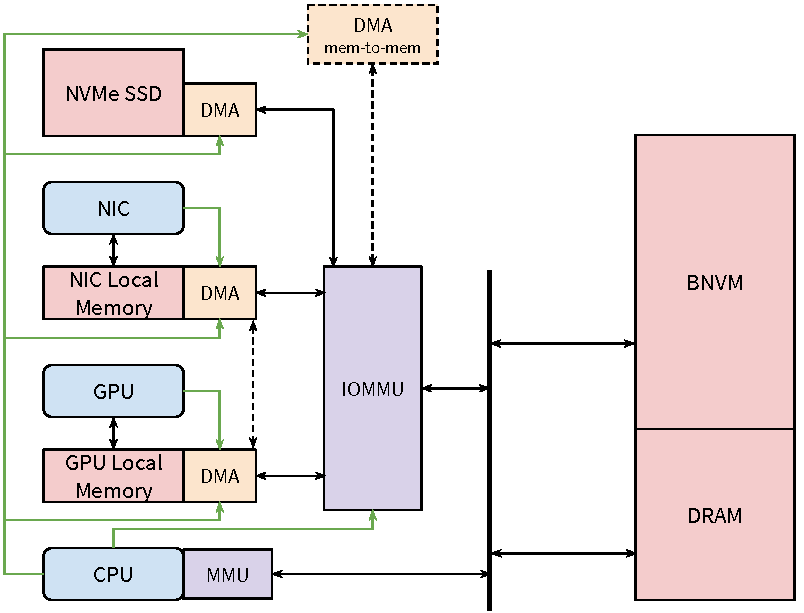
\includegraphics[width=\linewidth]{fig/sys_arch}
        \caption{Our expected system architecture. Solid black lines indicate data paths, green lines
            indicate administration paths. Dashed lines and boxes indicate potential future data paths and hardware
            that may become ubiquitous with these new hardware trends.}
        \label{fig:sys_arch}
    \end{SCfigure}


    A second trend is a consequence of improved fabrication techniques and shrinking feature
    sizes---hardware controllers are increasing in complexity, offering more autonomy from the CPU,
    off-CPU processing capabilities, and better parallelism. Hardware interfaces reflect the controller
    complexity expected of devices; for example, AHCI controllers improved request queuing over ATA, and DMA
    allows hardware to copy data directly to and from memory independent from the CPU. NVMe
    expands the responsibility of controllers again, adding deeper and parallel command queues, requiring
    devices to multiplex requests themselves and allowing them to exploit the parallelism of access
    available in SSDs. We expect these trends to continue, resulting in more programmable hardware
    devices that are able to act on shared, global memory with more autonomy.

    These changes are coupled with a shift in focus for how data moves throughout the system.
    Traditionally, data is considered to move into main memory for computation by the CPU, followed by
    storage to persistent memory (through a disk or SSD controller) or moved out onto the network
    (through a network controller). Figure~\ref{fig:sys_arch} shows a different model, where data moves
    through the system more fluidly. With more complex controllers and off-CPU processing, we expect
    non-traditional data paths to become more common. Say, for example, a packet arrives at the NIC
    containing compressed data for GPU processing. A traditional system would move the compressed data
    into main memory, decompress it using the CPU, and move it into GPU memory for processing. Instead,
    we could see a dedicated compression chip in the NIC whose job it is to decompress incoming data.
    That data could then be moved directly between the NIC's buffers and the GPU memory (the dashed
    line), without involving the CPU and main memory at all. This both reduces copies and frees these
    resources for other uses.
}


\subsection{Interconnect Technologies}

\section{Why Now?}

\todo[inline]{This will take some strong arumentation.}

\chapter{The Demands of Software}\label{ch:softwaredemands}

\begin{chabstract}
    This chapter will focus on software, the needs of software we must address, and the perspective of systems
    programming, putting the hardware trends we spoke of last chapter into context. We will discuss the problem of
    ephemeral context and discuss how persistence and RPC have shared characteristics and concerns.
\end{chabstract}

At their core, applications perform computation on in-memory data. Yet much application complexity is tied up in the
infrastructure surrounding that computation, for example, in managing persistent state and in performing serialization.
Additional work done by the program (or by the operating system on behalf of the program) that is merely in service of
setting up the computation and not the computation itself is considered \emph{overhead}. It is the goal of this work to
reduce that overhead in two ways: improving performance and reducing complexity. To do this, we need to understand where
overhead comes from, which elements are fundamental, and which are not.

\section{The Old Ways and ``Systems Programming''}

Current operating system interfaces are a poor fit for the trends and hardware requirements we discussed last chapter.
File \texttt{read} and \texttt{write} interfaces, originally designed for sequential media and later expanded for
block-based media, require significant kernel involvement and serialization, violating both the requirement to reduce
kernel involvement, and the need to reduce code paths around accessing data. Figure~\ref{fig:cycle} shows a fairly
common data path for an application that operates on (and perhaps mutates) some persistent data. First the data is
loaded explicitly into memory, either in a streaming fashion or as a whole file, followed by the application manually
deserializing it into an in-memory form. Once this is done, the program may commence its actual purpose---to perform
computation, hooray---after which the results are serialized and placed back onto disk with an explicit store operation.

\begin{SCfigure}
    \centering
    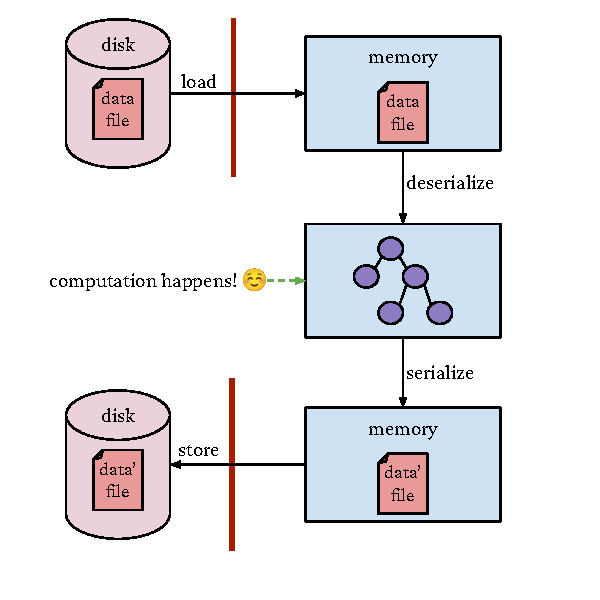
\includegraphics[width=\linewidth]{fig/cycle.pdf}
    \caption{The ``standard cycle'' of systems programming. We start with some persisted data, explicitly load it from disk into memory, deserialize it, compute on it, reserialize it, and explicitly store it back to disk. Note that the vast majority of this diagram depicts stuff other than the actual computation. The thick red lines depict persistence boundaries, across which data exists in different contexts and assumed lifetimes.}
    \label{fig:cycle}
\end{SCfigure}

Let's consider the case of from Chapter~\ref{ch:farout} of faster, closer persistence.
In the past, the time spent in manually loading and unloading
data, in transforming it between an on-disk form was an acceptable overhead, since the cost to access the disk was slow,
and those explicit load and store disk operations were going to be issued anyway. But when these operations overshadow
%% TODO cite more examples
device access time, the overhead quickly becomes unacceptable. As devices become faster and as applications process more
and more data, we find that more and more of our processing time is spent here. Applications can spend as much as 70\% of the processing
time~\cite{trims} deserializing and loading data into main memory at request time. Reducing this overhead would save
both in program time but also in \emph{programmer} time. Simplifying applications by removing the need for serialization
helps programmers by removing the need to maintain multiple data formats and the transformation code to move data
between those formats.

\subsection{The Context Problem}

If we look closely, the cycle in Figure~\ref{fig:cycle} can represent more than just processing files. It works
equally well for receiving data from a network and sending back a response (microservices and servers in general), for
applications in a traditional \texttt{pipe}line, \etc\sidenote{Those who sit high atop their \unix throne claim that text is a universal communication language. Yet anyone
    who has actually had the misfortune of parsing the output of even a moderatly complex \unix tool can realize that
    systems programming here involves just as much serialization and processing work as anywhere else---or else involves
    doing computation directly on C strings, a fate I would not wish upon my worst enemy.
}. But why do we spend so much time and effort with serialization and explicit I/O? Because the POSIX abstractions
fundamentally bifurcate our programming model in two:

\begin{enumerate}
    \item \textbf{Local Context} contains data that is limited to a single domain, for example in-memory data accessed
          via virtual addresses by a single process, or the domain of file descriptors. Data in a local context is typically
          operated on ``directly'' since it's usually in memory. Most importantly, though, the data isn't \emph{shared} with
          other domains, and it is ephemeral---its lifetime is tied to the context it is in.
    \item \textbf{Global Context} contains data that is shared across all the domains. Typically this covers data stored
          on disk or other stable storage. Data in a global context is usually stored in some serialized format and can
          be accessed by multiple domains simultaneously. The lifetime of data herein is, in the limit,
          infinite\sidenote{Even in the global context, we traditionally separate local storage and network storage.
              That separation can be eroded depending on the programming model, however, as we will discuss later.}.
\end{enumerate}

These separate contexts give rise to the need to transform data between them and to be explicit about marshalling data
across the boundary. The primary reason for the need for transformation has to do with \emph{data references} and
\emph{naming data}. For example, when applications operate on in-memory data, references take the form of virtual
addresses---pointers refer to specific locations within the virtual address space. The virtual address space is
ephemeral---it's tied to a specific process. But \emph{persistent} data is \emph{not} ephemeral! By definition it is
accessed by multiple processes, either over time (different invocations of the same process), or across space (shared
between multiple processes), or both. In either of these cases, virtual addresses cannot be used, since those addresses
may not agree across different contexts. So when sharing memory, any references to local context data must be
transformed into something that can be interpreted within the global context.

More generally, we often lock data access behind context that is tied to a shorter-lifetime actor, leading to
unnecessary indirections and extraneous work that the program must perform.
This is illustrated in how data relationships are typically handled, either:
\begin{enumerate}
    \item \textbf{Explicit, context-sensitive.} As we saw with virtual address pointers,
          references between data are encoded explicitly but rely on context provided by
          the ephemeral process abstraction. These references cannot be reliably shared between
          applications and across nodes which do not have the context necessary to interpret them.
    \item \textbf{Implicit.} Many data relationships are implicit in applications.
          Although there is a relationship between \texttt{/etc/shadow} and \texttt{/etc/passwd},
          it is not explicit. This limits interoperability between programs, prevents
          relationship discovery, and results in a brittle environment if these files are
          moved or replaced.
    \item \textbf{Explicit, via mediators.} Relationships can be encoded explicitly without
          ephemera if we use a global name resolution service. For example, an HTML
          file can refer to a style sheet by name. However, this presupposes the existence (and
          availability) of a global mediator and restricts programs from agreeing on the identity
          of data behind a reference without complex inter-networking and expensive global coordination.
\end{enumerate}

In our view, the complexity of these mechanisms is a symptom of a more fundamental problem: access to long-lived data
is unnecessarily mediated via ephemeral actors.
We advocate a violent break from this actor-centric model of data access, in favor of a model that elevates \emph{data}
as the systems' first-class citizen.  Doing so will require \emph{explicit
    context-free} references via globally unique identifiers (GUIDs) that name data objects. These
references are independent of context (\eg process) that operates on them, and require that all context necessary to interpret references
be stored within the data itself. Of course, we still need some understanding of
context-sensitive relationships, for example late-binding of names. We do this via a
``two-level'' naming system in which GUIDs are \emph{authoritative} names to which we can bind
additional names for purposes like local references, changing data identification, and discovery
(see Sections \ref{sec:implementation} and \ref{sec:latebinding}).

Viewing the past through the lens of the present, it was \emph{always} a mistake to entangle the context required to access
and manipulate data with ephemeral actors.  However, in the days of slow networks, spinning disks and small memories,
it was possible to hide these complexities and inefficiencies.  For one thing, disk-based I/O led to a model of sharing in
which long-lived data and computable data were stored in different \emph{kinds} of memory, in different formats (due to serialization),
with different reference formats (e.g., file names vs. virtual memory pointers).
The filesystem was a natural location to place the various hacks that were required to paper over the reality
that interacting with long-lived data required figuring out how to name the short-lived processes that were the primary
citizens of the operating system.

Needless to say, a disaggregated system model---one in which a particular data reference may
ultimately point to data on a different node from the one observing the reference---exacerbates all of these problems!
Two different nodes that observe the same data reference should agree on what data is
being referred to, and by the same token, an individual node observing two different data references
should be able to determine if they point to the same data. This asks the question of \emph{how}
to encode these explicit context-free data references while remaining efficient and avoiding global
coordination. We will discuss and answer these questions in detail in Chapters~\ref{ch:global} and \ref{ch:invariant}.


\section{Retrofitting POSIX?}

While I am arguing strongly that a clean-break reimagining is needed, it is worth considering what an incremental
approach might look like. For example, the problem of direct access might be solved to some extent by \texttt{mmap}, the
problem of global references could be solved by traditional pointer swizzling built atop \texttt{mmap}, \etc. We could
even combine this with RDMA to gain a \ac{dsm} model.

The \texttt{mmap} system call attempts to hide storage behind a memory interface through hidden
data copies. But, with \NVM, these copies are wasteful, and \texttt{mmap} still has significant kernel
involvement and the need for explicit \texttt{msync} calls. ``Direct Access'' (DAX)
tries to retrofit \texttt{mmap} for \NVM DIMMs by removing the redundant copy, but this \emph{still}
fails to address the problem of global context and in-memory data structures for persistent storage.
Operating on persistent data through \texttt{mmap} requires the programmer to
use either fixed virtual addresses, which presents an infeasible coordination problem
as we scale across machines and is fundamentally unportable, or virtual addresses directly, which are ephemeral and require the
context of the process that created them.

Attempting to shoehorn \NVM programming atop POSIX interfaces (including \texttt{mmap}) results in
complexity that arises from combining multiple partial solutions. Given some feature desired by an
application, the \NVM framework can provide an integrated solution that meshes
well with the existing support for persistent data structure manipulation and access, or it can
fall-back to POSIX resulting in the programmer needing to understand two different ``feature
namespaces'' and their interactions. An example of this is naming, where a programmer may need
to turn to the filesystem to manage names in a completely orthogonal way to how the \NVM frameworks handles
data references. For example, PMDK, a \NVM programming library, relies on a filesystem for naming and initial access to
persistent memory objects, resulting in different kinds of references, feature sets from filesystems
being applied (like security) while others are not (data access), and the complexity of
understanding how the PMDK abstractions interact with the POSIX ones. Instead, our model prefers to
build legacy support atop new abstractions (as we will see in Section~\ref{sec:legacy}), and avoid falling back to legacy
models for persistent data access.

Additionally, models that layer \NVM programming atop existing interfaces often fail to facilitate effective persistent data sharing and
protection.  PMDK, for example, makes design choices that limit
scalability, since its
data objects are not self-contained and do not have a large enough ID space, resulting
in the need to coordinate object IDs across machines, a problem we will explore in detail in Chapter~\ref{ch:global}. For the same reason,
although single-address space OSes~\cite{chase:tocs94} somewhat address requirement R1, they do
not consider both requirements at once, nor do they provide an effective and scalable solution to
long-term data references due to that same coordination complexity (as we will discuss in Section~\ref{sec:historical}).




\section{Remote Procedure Calls}

One major aspect of systems programming, particularly in distributed systems, that isn't covered by the diagram in
Figure~\ref{fig:cycle} is RPC. We typically use RPC as a mechanism for decomposition in distributed systems, allowing us
to break design problems down into smaller, re-usable parts that hide implementation details and are more easily debugged.
Decoupling components with RPCs allows them to scale
independently---in principle, developers need only agree
on a common interface and message format to leverage the
benefits of software decoupling. Yet, in reality,
RPCs enforce strict interface constraints and often
trade adaptability (narrow interfaces are harder to evolve) for
simplicity (narrow interfaces limit cross-component interactions),
ultimately hampering the goal of scalability.


The chief problem with RPCs is that they are fundamentally location-
and compute-centric: RPCs force a
programmer to decouple an application by explicitly separating the
computational endpoint or \emph{location} where a function is invoked
from the location where the function executes.  As a consequence, they are
well-suited to a relatively narrow set of use cases in which
function arguments (which flow from invoker to executor) and
returns (which flow back) must be serialized and sent in their
entirety, and hence are small, and in which reference data must be
located on the executor.


Many scenarios would benefit from decoupling but are simply not feasible using existing RPC
mechanisms. For example, the invoking endpoint may have abundant data but limited
compute, the invoker may wish to traverse a remote data structure, or the invoker may wish to
refer to data that they lack privileges to read. Rapidly growing model sizes, privacy concerns, and the proliferation of last-mile
model customizations all exacerbate the issue.
To mitigate the problem of location-centric RPCs, data center
operators often deploy discovery services, load balancers, or other
forms of middleware~\cite{eisenbud16,katran,tibco,kreps11,mq}. These
extra indirection layers make the execution endpoint abstract, but at
the cost of increased latency and added system complexity. Moreover,
we argue that such systems do not address the fundamental problem,
which is \emph{we need a more general mechanism for module
    composition in distributed systems}.

\subsection*{Motivating Example}

To illustrate the poor fit of RPC as a decoupling mechanism for some classes of applications,
consider an example from the distributed inference problem for edge devices. Here,
sensors in mobile devices with modest processing and storage resources (\eg mobile phones
or autonomous vehicles) are the source of observations used both for training and inference.
Recent work has focused on decoupling and distributing machine learning training across edge
and cloud resources to minimize client-perceived latency, provide privacy guarantees, and
maximize server-side throughput~\cite{federatedml,singh2019detailed}.

In this example, we focus on the inference problem that arises in response to device input.
Ideally, small models trained in the
cloud (via a methodology such as federated learning) are periodically shipped in their entirety to
edge devices, which perform local inference.  Several trends are upsetting this model. The first
is the aggressive growth---roughly 10$\times$/year---of models, in particular language models.
In 2018, the largest machine translation models at Google were 8.3 billion
parameters~\cite{megatron}; a mere two years later, the largest models exceeded 800 billion parameters!
Inference on sparse giant models which far exceed device resources must be performed server
side, where model serving presents a substantial throughput bottleneck. This is further
compounded by last-mile model customization for end users, in which inference tasks
for different devices \emph{must} be performed on slightly different models.  As much as 70\%
of the processing time~\cite{trims} for these model-serving applications is spent deserializing
and loading the sparse personalized models into main memory at request time. Finally, users prefer
local models remain local due to confidentiality concerns.

Consider a concrete example (Figure~\ref{fig:rpccopy}) that is bedeviled by all of these complexities at once. A mobile device,
Alice, in possession of a locally-trained model and an activation, wishes to perform a
classification task that requires a partition of a sparse global model, located on cloud resource
Bob. Further, imagine that Alice cannot perform the inference locally, either because the global
model fragment is too large or because she has inadequate local compute. Finally, imagine that Bob
is overloaded, while a separate cloud resource, Carol, is mostly idle.


\begin{SCfigure}
    \centering
    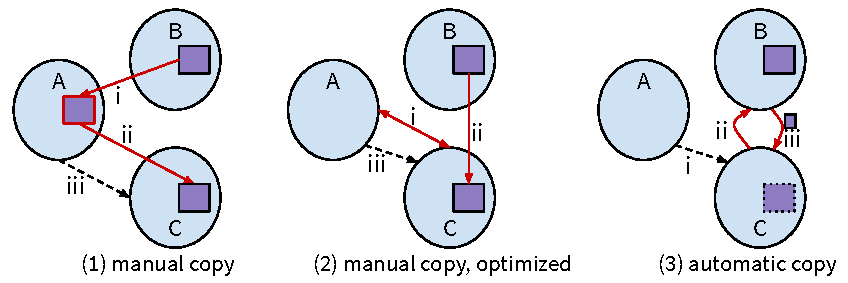
\includegraphics[width=\linewidth]{fig/copy}
    \caption{Rendezvous of data and compute. Solid red arrows are additional
        infrastructure-level tasks that are not fundamental to the requested computation.}
    \label{fig:rpccopy}
\end{SCfigure}

An ideal solution will minimize the latency Alice perceives and maximize the throughput offered
by both Bob and Carol, all while satisfying capacity constraints of each. It is easy to see
that while this application requires decoupling, RPC is the wrong abstraction in terms of performance,
expressivity, and flexibility.  Data movement---whether from storage to DRAM on Bob or from Bob
to Carol---requires costly serialization. If moving the data to Carol and performing
inference there is the optimal solution, the application logic on Alice must orchestrate this
infrastructure-level concern, either by pushing the data through Alice (Figure~\ref{fig:rpccopy} (1), a na\"ive solution)
or having the RPC executed
on Carol address Bob directly and pull (Figure~\ref{fig:rpccopy} (2)).
Both (1) and (2) require additional logic on Alice
to work---the programmer had to perform the infrastructure level task of data
movement.  Fundamentally, these issues arise because the system's core abstraction is
location-based---the programmer is forced to manually orchestrate machines or resort to
costly copying.
Further,
heterogeneity among end devices makes the ``hard-coded'' data movement strategy
brittle:
a subsequent classification request from client device Dave will be forced to run inference
on the server side even if it is equipped with the resources to do the work locally.

Figure~\ref{fig:rpccopy} (3) is more ideal. The first step is for
the computation to move to Carol instead of first moving data in preparation.  This may seem like a
minor point, but it is not---by specifying \emph{up-front} the computation we want to perform, we
open the door for lower-level optimization to examine our requests before we go around manually
moving data.  In fact, the programmer may not be directly asking Carol to perform the
computation; instead the placement decision would be made by the system. Once the code starts
executing, we can then move data on demand instead of having to move the entire
object.
Note that this matches the same requirements we discussed above with respect to context---data references must
be \emph{context-free} and global. With the ability to name data in a global context, we not only reduce the need for
serialization, but we also gain the ability to pass by \emph{reference} instead of by value.


\paragraph*{Patterns of RPC.}
%
While RPC is a poor fit here, there are applications for which RPC provides adequate decoupling.
RPC shines in situations where decoupling in the application meshes well with having little data
movement, where an RPC endpoint either fronts large data, large compute relative to the invoker, or
some combination, with \emph{small} arguments and return \emph{values}.
But call-by-small-value is a significant constraint, and there are many
classes of applications that do not fit.
We cannot paper over this problem, either.
Because
RPC is disconnected from a global notion of data identity, we either \emph{cannot} do
call-by-reference (because references must cross machine boundaries) or we must shoehorn this
functionality into the application logic and the RPC's APIs, resulting in brittle, repetitive,
complex code to deal with the coordination, caching, and prefetching that
comes from distributed data and global references when data moves.

The ``good'' use cases of RPC are ones in which code and data
co-location has already been preordained by initial decoupling (after which it is rigid) and
data transfer is minimal---often manifesting as something like a fronted key-value store service. This restricts
code mobility (as it accounts for no change to decoupling later), and requires a myriad of RPC calls
to implement all the ways a programmer might wish to view data (one need only look at the many S3
APIs available as an example).
If we limit ourselves to traditional RPC, any situation (such as the one discussed in
Section~\ref{sec:example}) that does not fit this pattern either results in expensive data movement
and complex application logic, or it must be dismissed altogether and the application redesigned.
By allowing applications to pass data references instead of just values, and by making data
references a first-class abstraction in the OS and the network, applications become much simpler to
express efficiently, even for what would be considered pathological cases for RPC.

\paragraph{A Counter to a Defense of Serialization}

A common response at this point is to point out that serialization serves several other purposes, such as ensuring
portability between environments that use different definitions of (\eg) \texttt{int} in C, or different machine
architectures that differ in endianess. I find these defenses weak. Firstly, for worrying about different ABI of types,
this is already a problem when sharing memory, and is a solved one. Many languages offer support for fixed-width values
and have explicit FFI functionality\sidenote{And continuing in the modern day with C's type system is a complete misstep
    anyway.}. As for endianess, much of the modern world uses little endian, and places that use big endian (networks) don't
really care about the data they are passing, they just worry about protocol headers. In any case, both of these issues
are problems that we can (and regularly do) solve at the language level.

And furthermore, there is nothing fundamentally tying these elements to the idea of global context and references, so
even if they weren't concerns at all, we would still need to serialize data as it moves across contexts. Our approach
is to solve the fundamental context problem that motivates serialization now, and solve the smaller problems that got
mixed into serialization at a higher level.

\begin{chconc}[So, What Does This All Mean (part 2)?]

    Software is growing in complexity, software is becoming more and more distributed with higher and higher demand for
    concurrency as it is asked to process more and more data.
    As we saw both with accessing persistent data and in RPC, serialization takes a huge amount of processor time and a
    large chunk of an application's complexity budget. Relying on kernel crossings to perform I/O is costly, particularly if
    we reduce or remove the need for serialization. Having to resort to call-by-small-value when trying to effect
    computation remotely severely limits the expressability of distributed applications, and can have a negative impact on
    decoupling and modularity---the very thing that RPC is supposed to solve.

    If we are to provide a solution by way of a new programming model and OS abstractions, it must be one that both solves
    the problems that software has and provides abstractions that best take advantage of the new hardware. Mere incremental
    change will not get us there. Fortunately, what we are seeing is a confluence of software demands and hardware trends.
    The hardware is becoming better equipped to support high concurrency, distributed applications that can share memory
    within a larger context. To take best advantage of hardware, we must reduce kernel involvement and move towards a global
    address space of in-memory data---which is exactly the solution that cuts down the overhead of serialization and system calls
    to zero. The remainder of this thesis will discuss how we can use this global address space, with first-class support
    for references, to solve not only the problems of persistence and the systems programming cycle, but also that of
    computation mobility, factoring out complexity, and providing simpler, higher performance applications. But to do
    this, we will need an operating system built for that purpose.

\end{chconc}
\cleardoublepage
\part{A Data-Centric OS}\label{pt:datacentric}

\chapter{The Data-Centric Approach}\label{ch:datacentric}

\section{An Opportunity Arises}

\unedit{

    Our core vision is to combine the code mobility of RPC with the flexibility offered by
    DSM-like models in a global address space with global references as a first-class abstraction. By
    imbuing data with fundamental identity and pushing an understanding of data references into the OS
    and the network, we can leverage aspects of content-based networks to reduce the coordination
    typically required in a shared, distributed address space. The programmer is then free to express
    their computation through references to code to run on some \emph{references} to data, instead
    of needing to serialize and copy \emph{values} for arguments.
    Today, developers are often forced to implement functionality such as caching, prefetching, and
    manual data movement in preparation for some operation.
    With data references as a common
    language between the OS, the network, and applications, we can move this infrastructure-level functionality
    out of the application and back \emph{into the infrastructure} where it belongs.
}

\section{A Common Language}



\unedit{
    We cannot store virtual addresses in persistent data, so we need a new way to name a word of
    persistent memory: a \emph{persistent pointer}. The persistent pointer encodes a persistent
    identification
    of data (\S~\ref{sec:invariant_pointers}) instead of an ephemeral address,
    allowing any thread to access the desired word of memory regardless of
    address space.
    This approach dramatically improves programmability, as programmers
    need not worry about the complexity of referring to persistent data with ephemeral constructs,
    improving data sharing between programs and across runs of a program. \Twizzler still makes use of virtual
    memory \emph{hardware} to provide isolation and translation, but persistent data
    structures should not be written in terms of virtual addresses.


    \paragraph{The Death of the Process.}
    Processes as a first class OS abstraction are, like virtual addresses, unnecessary; a traditional process couples
    threads of control to a virtual address space, a security role, and kernel state.
    %an environment for a set of threads to operate in.
    However, with the kernel removed from
    persistent data access, much of that kernel state (\eg file descriptors) is unnecessary,
    leading to a decoupling of mechanisms:
    nothing fundamentally connects a virtual address space
    (a piece of ephemeral context used to access data) and a security context (\emph{what} data
    threads may access).
    Instead, a data-centric OS can keep the good parts of a process but \emph{separate} virtual address
    translation and security roles, allowing threads to select one of each as needed.


    %\footnote{Of course, we do not want to throw out \emph{good} parts of a process. Mechanisms like
    %protection, shared memory, and (in some cases) hierarchical responsibility still have their uses,
    %but do not need to be coalesced into a single, rigid abstraction. Their separation would have
    %significant effects on the POSIX model, but our model, but our model, built from clean abstractions,
    %can make use of gained flexibility (as we will see in \S~\ref{sec:eval}).}.


    % maybe move this to 4.3?
    The process abstraction is just one example. Persistent data access plays a key role in OS
    abstraction design, and we need to avoid complexity arising from combining old and new interfaces.
    Hence, we need to consider the
    wide-reaching effects of changing the persistence model on \emph{all} aspects of the system, not
    just I/O interfaces. \NVM gives us an opportunity to design an OS around the requirements
    of the target programming model instead of trying to mold support libraries around existing
    interfaces. While it is important that we provide support for legacy applications,
    it is these applications that should be relegated to support libraries; new applications built for
    the programming model should get first-class OS support.
}

\unedit{
    \subsection{Computation and References}

    First-class support for call-by-reference instead of by-value allows an invoker to refer to data that \emph{they
        do not have locally}. This allows greater freedom in the interface design between decoupled components.
    Figure~\ref{fig:rpccopy} shows possible solutions to a problem like the
    example in Section~\ref{sec:example}, wherein an operation is scheduled to run on Carol using data
    currently located on Bob. Part (1) shows the na\"ive approach where the invoker copies the data
    locally (step i) before forwarding it to Carol (step ii) and eventually invoking the intended computation
    (step iii).  In an attempt to alleviate an unnecessary copy, we could implement an additional
    RPC on Carol that allows it to copy data over from Bob itself (steps i and ii in part (2)) before we
    finally invoke our computation. Both (1) and (2) require additional logic on Alice
    to work---the programmer had to perform the infrastructure level task of data
    movement.  Fundamentally, these issues arise because the system's core abstraction is
    location-based---the programmer is forced to manually orchestrate machines or resort to
    costly copying.

    Figure~\ref{fig:rpccopy} part (3) is closer to our vision. The first step is for
    the computation to move to Carol instead of first moving data in preparation.  This may seem like a
    minor point, but it is not---by specifying \emph{up-front} the computation we want to perform, we
    open the door for lower-level optimization to examine our requests before we go around manually
    moving data.  In fact, in our model the programmer would not be directly asking Carol to perform the
    computation; instead the placement decision would be made by the system. Once the code starts
    executing, we can then move data on demand instead of having to move the entire
    object.  Of course, the implementation is significant---without a global address space like
    the one we are proposing, implementing (3) would require brittle code that either tightly couples
    Carol and Bob or forces Alice to participate in the data movement by asking it to provide a
    location-based reference to the data on Bob\footnote{Aside from the complexity, this also
        opens up TOCTTOU errors.}.


    \begin{figure}
        \centering
        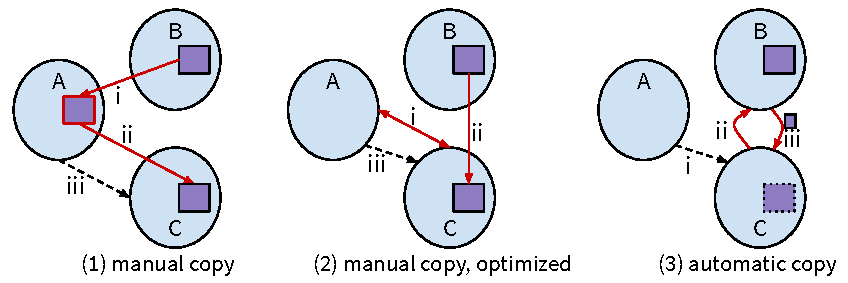
\includegraphics[width=0.9\columnwidth]{fig/copy}
        \vspace*{-5mm}
        \caption{Rendezvous of data and compute. Solid red arrows are additional
            infrastructure-level tasks that are not fundamental to the requested computation.}
        \label{fig:rpccopy}
        \vspace*{-4mm}
    \end{figure}

    As discussed previously, the ``good'' use case of RPC is one where code and data
    co-location has already been preordained by initial decoupling (after which it is rigid) and
    data transfer is minimal---often manifesting as something like a fronted key-value store service. This restricts
    code mobility (as it accounts for no change to decoupling later), and requires a myriad of RPC calls
    to implement all the ways a programmer might wish to view data (one need only look at the many S3
    APIs available as an example).
    If we limit ourselves to traditional RPC, any situation (such as the one discussed in
    Section~\ref{sec:example}) that does not fit this pattern either results in expensive data movement
    and complex application logic, or it must be dismissed altogether and the application redesigned.
    By allowing applications to pass data references instead of just values, and by making data
    references a first-class abstraction in the OS and the network, applications become much simpler to
    express efficiently, even for what would be considered pathological cases for RPC.

    \paragraph*{Serialization.}
    %
    In traditional host- and process-centric systems, virtual memory spaces are private to a
    program instance and thus addresses are too. As a result, we serialize any data that passes between
    hosts (and sometimes even processes) because memory addresses on one host do not translate to any
    other host. However, in our model, pointers refer to data within the \emph{global} address space,
    and thus a data structure containing pointers can be copied from one host to another with merely a
    byte-level copy, alleviating 100\% of the loading overhead discussed in Section~\ref{sec:example}
    and leaving only data transfer costs, which are fundamental. These transfer costs, however, can now
    be included in cost-models when making placement decisions more easily, as they do not need to take
    the additional loading time into account.

}


\section{The Design Space}



\unedit{
    % maybe this goes in into or 4.1?
    Operating systems provide abstractions for data access that reflect the hardware for which
    they were designed. Current I/O interfaces and abstractions reflect the structure of mutually
    exclusive volatile and persistent domains, the hallmarks of which are heavy kernel involvement for
    persisting data, a
    need for data serialization, and complexity in data sharing requiring the overhead of
    pipes or the management cost of shared virtual memory. However, the introduction of low latency and directly
    attached
    \NVM into the memory hierarchy requires that we rethink key assumptions such as
    the use of virtual addresses, the kernel's involvement in persistent I/O, and the way that
    programs operate on and share persistent data~\cite{faraboschi:hotos15}.
}


\unedit{
    These characteristics imply two basic requirements for OSes
    to most effectively use \NVM:
    \begin{enumerate}
        \item[(R1)] \textbf{Remove the kernel from the persistence path.}
            This addresses both
            characteristics. System calls to persist data are costly; we must provide
            lightweight, direct, memory-style access for programs to operate on persistent data.
        \item[(R2)] \textbf{Design for pointers that last forever.}
            %This is a direct
            %consequence of applications using in-memory data structures in persistent memory.
            Long-lived data structures can directly reference persistent data, so
            pointers must have the same lifetime as the data they point to.
            Virtual memory mappings are, by contrast,
            ephemeral and so cannot effectively name persistent data.
            Persistent data is, by definition, accessed by multiple actors, both
            simultaneously and over time, and thus must be stored in a form that is conducive to sharing without
            needing the ephemeral context associated with a particular actor.
    \end{enumerate}
}


\unedit{
    We call an OS that meets both requirements R1 and R2
    \emph{data-centric}, as opposed to current OSes, which are \emph{process-centric}.
    Operations on persistent, in-memory data structures are the primary functions of a data-centric OS,
    which tries to avoid interposing on such operations, preferring instead to intervene only when
    necessary to ensure properties such as security and isolation. To meet both of these requirements
    a data-centric OS must provide effective abstractions for identifying data independent
    of data location, constructing persistent data relationships that do not depend on ephemeral
    context, and facilitating sharing and protection of persistent data.
}


\unedit{

    While considering a single machine as a distributed system\footnote{While the system is
        distributed, and contains communicating entities, it is not \emph{truly} a traditional
        distributed system, since a single machine does not include partial-failure semantics (and the
        cases where it does are rare enough that they may be largely ignored); often a partial failure
        of a component is instantly upgrade to total failure. However, the messaging semantics of
        distributed systems are present.} has been examined from the
    perspective of OS design~\cite{baumann:sosp09}, the extent to which we are proposing has not been.
    \emph{Each} device, including CPU sockets, acts like a component containing a local memory with
    \emph{direct} access to a pool of shared, persistent storage.

    Such a model has two significant implications:
    \begin{enumerate}
        \item Protection of data within this system is of utmost importance, considering how each of
              these devices
              could run an entire operating system with application suites. The green lines in
              Figure~\ref{fig:sys_arch} represent control paths, showing how memory access is administrated. Note
              that the CPU, while similar in some respects to other devices, is distinguished in that it sets
              security policies for the system\footnote{Only in supervisor mode; user-space applications can only
                  administrate devices that have been mapped into their address spaces.}. The \emph{enforcement}
              of those policies is handled by the MMU and the IOMMU, both of which apply a mapping of virtual
              addresses to physical addresses along with access restrictions.
        \item The addresses emitted by such devices are typically physical addresses that DMA engines
              operate on. However, similar to \observation~\ref{hetero-mem} above, emitting physical
              addresses has significant complications in our model, necessitating the need for hardware to
              abstract physical memory into an object-space as well. Current systems can implement this
              (along with protection) through the IOMMU for hardware devices and MMU for the CPU.
    \end{enumerate}

    These implications combined with \observation~\ref{hetero-mem} leads to another point:

    \observe{sls}{The CPU and devices must agree on a single, global abstracted view of
        shared physical memory, leading to a system-wide single-level store interface (shown in
        Figure~\ref{fig:log_sys_arch}). Protection is
        enforced by hardware devices such as the IOMMU, and devices can operate on data objects as
        opposed to physical memory directly.}

    In the case of specialized hardware running programs, this grants hardware better access to global
    memory because it does not need to coordinate and the system can trust it more (since the IOMMU can
    enforce security). For simple I/O controllers, like an NVMe device, it allows programming of such
    devices in a more efficient and simpler way---instead of translating object pages into physical
    addresses, it can issue DMA requests directly to object pages instead.


    \begin{figure}
        \centering
        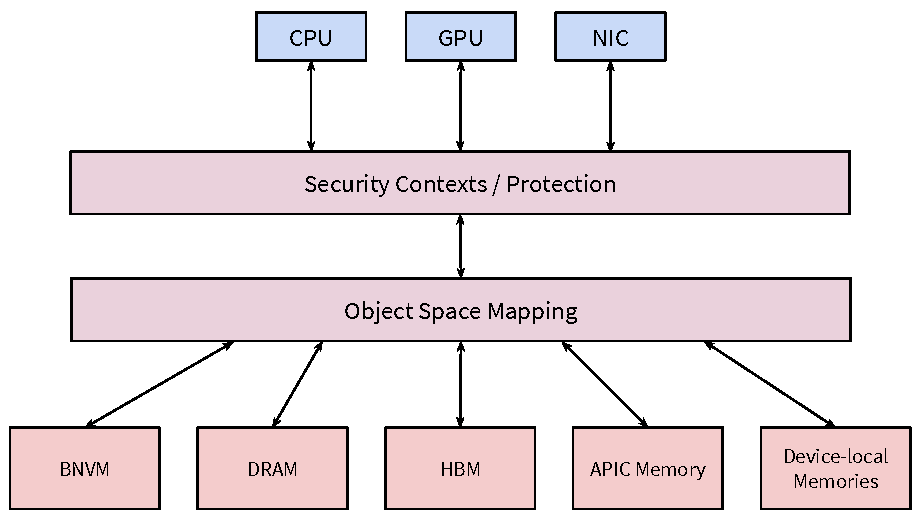
\includegraphics[width=0.7\textwidth]{fig/log_sys_arch}
        \caption{Logical view of the system architecture. Mapping hardware such as the IOMMU would allow
            \emph{all} devices to see a single-level store instead of raw physical memory.}
        \label{fig:log_sys_arch}
    \end{figure}


    An example of this would be if a NIC is processing data it received in a packet, and that data
    references data in another data object. If there were no abstraction layer, the NIC would need to
    either interrupt the CPU to ask where the data is, or it would need to keep a map of objects in
    physical memory itself. The latter adds to management costs of maintaining such maps for all
    hardware devices in the system when data placement changes, and the former results in performance
    degradation (due to interrupting the CPU) and requires additional management code to assist in
    making data transfers on behalf of the hardware devices\footnote{Many current devices today will
        still need this. However, we are planning for a system model in which it is less necessary. Many
        devices today fit this model, including some GPUs and special off-chip processing
        accelerators.}. This also leads to another \observation about data movement, since data
    processing decisions will need be made by devices autonomously:

    \observe{mem-to-mem}{Operating systems will need to provide a way for applications to specify data
        movement in a system declaratively, so that data movement decisions can be made largely without user
        involvement.}

    %A natural consequence of such a distributed system is heterogeneous computing, where we have
    %different types of processors accessing memory simultaneously. This could be as simple as an x86
    %processor and an ARM processor both operating on shared memory, where the system offloads
    %computationally nonintensive tasks to the ARM chip, but also encompasses our system design above.
    %For example, ARM GPUs can (and do) access global memory with cache coherence with the CPU (CITE).
    %The jury is still out on scaling-up cache coherence in this way, and systems will need to support
    %both devices that operate on only local memory and devices which operate on shared memory.



    The system design shown in
    Figure~\ref{fig:sys_arch} is not necessarily the end evolution of treating a single machine as a
    distributed system of components. We could imagine treating the CPU like any other component which
    accesses shared memory through a controller that itself enforces memory protections and mappings.
    However, such a model is easier to reach and program for as an evolution of our proposed system
    design presented here. Furthermore, Figure~\ref{fig:sys_arch} shows a system design that can be
    realized \emph{now}, allowing us to construct a real system to explore our goals.


}


\subsection{Hardware Versus Software}

\unedit{
    The challenges introduced by BNVM in mapping virtual addresses to physical
    addresses are the different lifetimes of data with respect to
    the references to that data and the heterogeneity of physical memory. Software and hardware have
    different requirements for this mapping, in the following respects:

    \begin{enumerate}
        \item[Latency.] Prior persistent data access schemes relied on system calls to
            operate on persistent storage. BNVM's low-latency can no longer tolerate the cost of those
            system calls. Instead, programs must have direct access to
            persistent data via load/store instructions. Similarly, hardware must be able to
            transfer data to and from BNVM using DMA.
        \item[In-memory data structures.] Direct access to persistent memory removes the loading and
            unloading cost, but we must \emph{also} remove the cost of data serialization: since
            persistent data is located in-memory, programs can operate on data as in-memory data
            structures using standard programming techniques. This change
            is not an issue for hardware, which treats data as a ``bag of bits''.
        \item[Data lifetime.] If persistent data is stored as in-memory data structures, then
            applications need a way to refer to data such that references have the same lifetime
            as the referenced data, a requirement that fundamentally arises from the need for
            to construct references that encode the relationships between data. Applications can store
            \emph{persistent pointers} that encode a more persistent name for data than an ephemeral
            virtual address.
            Again, hardware has no such requirement, since it neither constructs
            nor interprets relationships between data. Devices that need to consider data
            relationships do so in software running atop the hardware.
        \item[Mappings.] Both software and hardware must have a way of translating a
            %$\langle \mathit{object}, \mathit{offset} \rangle$ reference
            persistent pointer into a physical address.
            This mapping may change frequently as the OS changes allocation of physical
            pages to data (\eg, to persist a piece of data).
            %to objects, potentially moving objects in and out of BNVM (\eg, to persist an object).
            Hardware need only know
            %the mappings for a short time, and need not even know the ``canonical''
            %name for the object---
            %it simply needs to know
            how to access data in memory
            for a single operation. In contrast, software must have longer-term mappings, and must
            be able to support data shared between threads, potentially mapped into the threads
            in different places.
        \item[Memory heterogeneity.] Hardware and the operating system must know about different
            types of memory, \eg DRAM and BNVM.
            Software need only know how to allocate
            from the different types, and should not deal with other differences. Hardware, however,
            will need to know when data is moved between memory types if it wishes to correctly emit loads and stores
            requested by software.
    \end{enumerate}

    Our design must support appropriate abstractions for both software and hardware, facilitating the
    use of \emph{persistent pointers} to long-lived data for applications while providing hardware and
    the OS with the ability to move data in, out of, and around physical memory, preferably only using
    existing hardware functionality. We first abstract memory into \emph{objects},
    where related data with similar access semantics (\eg, an entire B-tree, where all nodes are subject
    to the same access control, \emph{etc}.) are placed in a single object and identified by
    a \emph{globally} unique ID. IDs are formed via hashing, partitioned allocation, or other methods that prevent collisions
    of IDs across machines with high probability.
    %A programmer could, for example, place an entire B-tree within an object (as the
    %tree itself has similar access control, etc.).
    %, or create a tree that spans multiple objects with
    %pointers between them.

    We propose two abstractions to provide effective access to objects for both hardware and software:
    a \emph{global object space}, which facilitates persistent pointers (discussed below), and a
    \emph{logical object space}, which allows hardware to address data without needing knowledge of the
    data's physical location. We split these abstractions and consider them different because of the
    different requirements discussed above; software must worry about reference lifetime, whereas
    hardware's access to objects is disconnected from persistence. On the other hand, today's hardware
    must worry about physical location of data, which (with BNVM) is now more
    likely to change over time.
}

\unedit {
    \paragraph{Hardware and Memory}

    The interface presented to hardware must enable interaction with a
    \textit{heterogeneous memory system} and support the abstraction of an object space rather than a
    collection of flat memory spaces. Unlike applications, hardware has no need for
    creating long-lived pointers to locations within objects. Rather, hardware must
    have the ability to transfer large chunks of objects to, from, and around memory, and must be able to
    manage different \emph{types} of memory, preferably in a way that is largely transparent to
    applications.

    Requiring hardware to access a global object space through a $\langle \mathit{object},
        \mathit{offset} \rangle$ tuple is unnecessary overhead and complexity---hardware need only ever
    access the ``working set'' of objects currently undergoing computation. Thus, our design abstracts
    the view from hardware of physical memory into a \emph{logical object space}, an address space that
    maps contiguous objects within it to physical memory pages, managed by the
    operating system. This solves the heterogeneity problem by allowing hardware to refer to data within
    objects instead of physical addresses, whose lifetimes are much smaller than the objects, and
    doesn't require hardware to emit (likely large) addresses for the global address space.

    While SASOSes are not a viable solution to the problem of persistent pointers, they are
    \emph{a} solution to implementing the logical object space.  Hardware, and the CPU, are
    directly connected, reducing the cost of invalidation and coordination of an address space.
    Additionally, this address space is \emph{intermediate} and hidden from programs---a virtual
    address is translated to the logical object space, after which the address is translated to a
    physical location (shown in Figure~\ref{fig:twolevel}). This translation for
    applications (after the virtual address translation) and that of hardware is the same, reducing the
    management complexity for the OS, discussed in Section~\ref{sec:os:addrspace}.

}


\subsection{Twizzler: A Point in This Space}


\unedit{
    The consequences of meeting the requirements of these hardware trends
    %and the consequences of those requirements
    define a bounded design space for data-centric OSes. We have
    chosen a point in that space and built \Twizzler, our approach to providing
    applications with efficient and effective access to \NVM. In the
    following section we will discuss how our four primary abstractions---a low level persistent object
    model, a persistent pointer design, an address space mechanism called \emph{views}, and a
    security context mechanism---achieve these goals of removing the kernel from the persistent data
    access path.
}


\unedit {
    There are several design principles that we believe a successful system must adhere to:
    \begin{enumerate}
        \item \textbf{Get the OS out of the way}
              Addressing \observation~\ref{os-out-of-the-way} requires removing kernel invocations from the
              common path of persistent data access. Instead, we provide applications with methods for
              accessing persistent data directly as in-memory data structures, thereby removing the
              overhead of kernel boundary crossings. Note that this necessarily implies a shared-memory
              style interprocess communication. When shared memory is not possible, however, the system
              must support some form of message passing.

              Such a model also addresses \observations~\ref{data-movement} and~\ref{mem-to-mem}, since
              by removing the kernel from the path of persistent, shared data access, hardware can more
              autonomously operate on data objects.

        \item \textbf{Orthogonal persistence} The emergence of BNVM will make persistence the norm
              rather than the exception, and so the programming model should have both \emph{persistence
                  by default} and \emph{transparent, implicit} persistence. However, in accordance with
              \observation~\ref{consistency}, applications will need to play a significant role in
              consistency of persistent data.

        \item \textbf{Single address space} We will provide a single address space of data objects to
              applications \emph{and hardware} called the \emph{object-space}. This addresses
              \observations~\ref{hetero-mem} and~\ref{sls} by abstracting
              different types of physical memory and allowing DMA transfers to refer to data within
              objects instead of physical addresses. Applications running on the CPU will, too, see this
              same address space, allowing references to more easily pass around the system. Additional
              benefits include:
              \begin{enumerate}
                  \item Allows devices to refer to object data without needing to be aware of where the
                        object is physically located. This is advantageous in a heterogeneous memory
                        hierarchy, since data may move often.
                  \item Simplified security policy: security policy can be defined for objects instead of
                        physical address.
                  \item More autonomous operation of devices: if the system can rely on security
                        enforcement via the IOMMU, these devices can securely access data in main-memory on
                        their own without needing to be reprogrammed often.
                  \item Simplified system programming: the unified data access model of Twizzler allows
                        programmers to write programs that operate on data
                        that can then run on any device, from the CPU to a NIC, without needing to
                        specialize their application.
              \end{enumerate}
              Of course, if a device (CPU or otherwise) wishes to provide additional layers of abstraction
              (such as segmentation or virtual address spaces) atop this single address space to ease
              programming, they may do so (to assist in addressing \observation~\ref{sasos}). Internally, however, the object-space allows hardware devices
              to agree on a way to reference that data within the system, regardless of where it may be
              physically located.
        \item \textbf{Data movement and security} should be handled declaratively, so as to not require invoking
              the CPU whenever such a decision needs to be made (\observation~\ref{mem-to-mem}).
    \end{enumerate}
}

\unedit{

    \Twizzler is a stand-alone kernel and userspace runtime that provides execution support
    for programs. It provides, as first-class abstractions, a notion of threads, address spaces,
    persistent objects, and security contexts. A program
    typically executes as a number of threads in a single address space (providing backwards
    compatibility with existing programming models), into which persistent objects are mapped on-demand.
    Instead of providing a process abstraction, \Twizzler provides \emph{views}
    (\S~\ref{sec:view}) of the object space, which formalizes the notion of ephemeral context within our
    model by allowing programs to map objects for access,
    and \emph{security contexts} (\S~\ref{sec:sec}) which define a thread's access rights to objects in the system.
    \Twizzler provides persistent pointers  (\S~\ref{sec:invariant_pointers}) for
    programs, as well as primitives to ensure crash-consistency
    (\S~\ref{sec:crash}). The thread abstraction is similar to modern OSes; the
    kernel provides scheduling, synchronization, and management primitives.
    Figure~\ref{fig:twz_sys_overview} shows an overview of the system
    organization and how different parts of the system operate on data objects.

    \begin{SCfigure}[b]
        \centering
        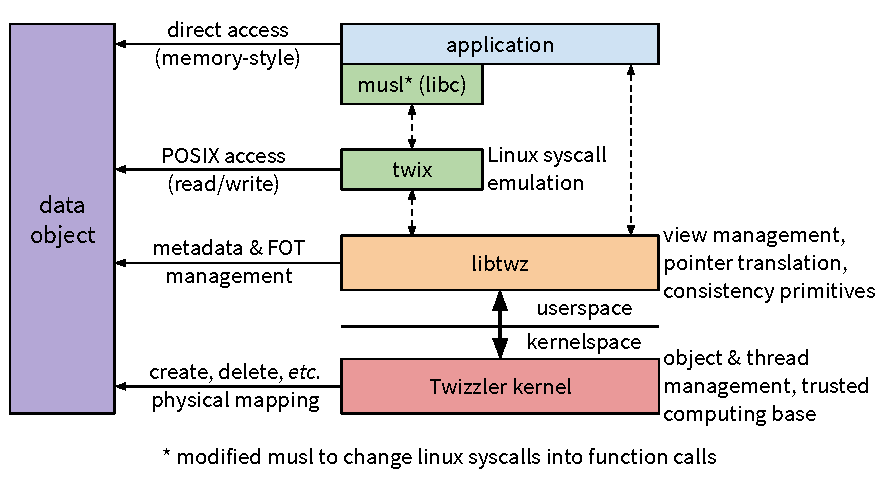
\includegraphics[width=\textwidth]{fig/sys_diag}
        \caption{\Twizzler system overview. Applications link to \texttt{musl} (a C library),
            \texttt{twix} (our Linux syscall emulation library), and \texttt{libtwz} (our standard
            library). Through \texttt{musl}, they may act on persistent data with POSIX interfaces,
            though we expect \Twizzler applications to operate directly on persistent data with
            memory-style semantics.}
        %They can directly access objects or they can use legacy POSIX methods.}
        %The \texttt{libtwz} library provides library-OS functionality and manages the
        %address space and kernel interaction. The kernel manages objects, schedules threads, and
        %enforces security by programming MMU hardware.}
        \label{fig:twz_sys_overview}
    \end{SCfigure}


    \Twizzler's kernel acts much like an
    Exokernel~\cite{Kaashoek,engler:sosp95}, providing sufficient services for a
    userspace library OS, called \emph{\libcore}, to provide an execution environment for applications.
    The primary job of \libcore is to manage mappings of persistent objects into the address space (\S~\ref{sec:view})
    and deal with persistent pointers (\S~\ref{sec:invariant_pointers}).
    \Twizzler also exposes a standard library that
    provides higher level interfaces beyond raw access to memory. For example, software that better fits
    message-passing semantics can use library routines that implement message-passing atop shared
    memory. \Twizzler's standard library provides additional
    higher level interfaces, including streams, logging, event notification, and many
    others. Applications use these to easily build composable tools and pipelines for
    operating on in-memory data structures without the performance loss and complexity of explicit I/O\@.

}

\section{A Historical Look}


\unedit{\label{sec:relwork}

    %The introduction of byte-addressable non-volatile memory presents an outstanding
    %opportunity to rethink the way that OS's handle memory and storage.

    % Working with new technologies often allows past, merely theoretical ideas a
    % chance to be practical.

    \Twizzler's design
    is shaped by fundamental OS
    research~\cite{corbato_introduction_1965,chase:tocs94,k42,engler:sosp95,Kaashoek,engler1995avm,engler1995exterminate},
    which,
    while approaching similar topics described in
    Section~\ref{sec:datacentric}, often did not consider \emph{both} design
    requirements simultaneously, resulting in an incomplete picture for \NVM.
    Recent research on building \NVM data structures~\cite{volos:asplos11,coburn:asplos11,condit:sosp09,debnath:vldb10,lu:tos16,hu:atc17},
    often focuses on building data structures that
    provide failure atomicity and consistency.
    In contrast, we explore how \NVM affects programming models while potentially improving performance.
    We draw from recent work on providing OS support for \NVM systems~\cite{caulfield:micro10} and work
    providing recommendations for \NVM systems~\cite{mehra:ipdps04}, integrating
    object-oriented techniques and simplified kernel design
    to provide high-performance OS support for applications running on a single-level
    store~\cite{shapiro:sosp99,bailey:hotos11}.

    % Our approach will leverage non-volatile memory characteristics to greatly
    % reduce the need for an OS stack and provide full system
    % resumability.
    %, we draw on prior object-oriented OS design work to
    %simplify the kernel using techniques developed in systems such as K42~\cite{k42}
    %and
    %Exokernel~\cite{kaashoek_application_1997, engler:sosp95}.

    %\subsection{Memory Model}
    \paragraph{Memory and Object Model}

    Multics was one of the first systems to use segments to partition memory and
    support relocation~\cite{bensoussan:sosp69,daley:cacm68}. It used segments to
    support location independence, but still stored them in a file system, requiring manual linkage
    rather than the automated linkage in \Twizzler. Nonetheless, Multics demonstrated that the use of
    segmenting for memory management can be a viable approach, though its
    symbolic addresses were slow.

    The core of \Twizzler's object space design uses concepts
    from Opal~\cite{chase:tocs94}, which used a single virtual
    address space for all processes on a system, making it easier to share
    data between programs. However, Opal was a single-address space OS, which is insufficient for
    \NVM~\cite{bittman:plos19,bittman:hotstorage19},
    and, while it resulted in a speedup of data transfer and sharing as well as interfacing with
    devices, it did not address issues of file storage and name resolution. It also
    still required a file
    system, since there was no way to have a pointer refer to an object with changing identity,
    whereas our approach
    of late-binding for pointers
    removes the need for an explicit file system.  Other single-address space
    OSes, such as Mungi~\cite{heiser:scse9314},
    Nemesis~\cite{roscoe:osr94}, and Sombrero~\cite{skousen:ipccc99}, show that
    single address spaces have merit, but, like Opal, did not consider how the use
    of \NVM would alter their design choices; in particular, how the use of fixed addresses
    results in a great deal of coordination that is unnecessary in our approach.
    OSes such as HYDRA~\cite{wulf:cacm74} provide functionality similar to cross-object pointers;
    however, in \Twizzler, we extend their use from procedures-referencing-data to
    a more general approach. Furthermore, they required
    heavy kernel involvement, an approach incompatible with
    our design goals.

    Single-level stores~\cite{shapiro:usenix02,shekita:uwtr956,dearle:cs94} remove the
    memory versus persistent storage distinction, using a single model for data
    at all levels. While well-known,
    ``little has appeared about them in the public
    literature''~\cite{shapiro:usenix02}, even since the EROS paper.
    Our work is partially inspired by Grasshopper~\cite{dearle:cs94}, AS/400, and orthogonal persistence systems,
    but while these are designed to provide an illusion of persistent
    memory, \Twizzler is built for real \NVM and focuses on providing a truly global object space with
    global references without cross-machine coordination.
    Clouds~\cite{dasgupta:computer91} implemented a distributed object store in
    which objects contained code, persistent data, and both volatile and
    persistent heaps. Our approach uses lighter-weight objects, allowing direct
    access to objects from outside, unlike Clouds. Software persistent
    memory~\cite{guerra:atc12}, designed to operate within the constraints
    of existing systems, built a persistent pointer system using explicit
    serialization without cross-object references, in contrast to \Twizzler.
    %In contrast,
    %\Twizzler develops mechanisms that leverage \NVM,
    Meza~\cite{meza:weed13}
    suggested hardware manage a hybrid persistent-volatile store with
    fine-grained movement to and from persistent storage. Since
    persistence in \Twizzler is to \NVM, we need not interpose on
    movement between storage and memory,
    instead simply managing memory mappings of persistent objects,
    reducing OS overhead.

    Recently, several projects have considered the impact of non-volatile
    memories on OS structure. Bailey,
    \etal~\cite{bailey:hotos11} suggest a single-level store design.
    Faraboschi, \etal~\cite{faraboschi:hotos15} discuss challenges and inevitable system organization
    arising from large \NVM, and we follow many of their recommendations.
    %and using
    %\NVM to ship a program as a checkpoint of a running process. 
    The Moneta
    project~\cite{caulfield:micro10} noted that removing the
    heavyweight OS stack dramatically improved performance.
    While Moneta focused on I/O performance, not on rethinking the
    system stack, we leverage their approach to reduce OS
    overhead as much as possible, even when the OS must intervene.
    Lee and Won~\cite{lee:hpcc13} considered the impact of \NVM on
    system initialization by addressing the issue of system boot as a way to restore
    the system to a known state; we may need to include similar techniques to
    address the problem of system corruption.
    Our work evolved from some earlier work where we laid the groundwork for abstraction requirements
    for both hardware and software for \NVM~\cite{bittman:hotstorage19} and a discussion on the
    implications of system-wide persistent data references~\cite{bittman:plos19}.

    \paragraph{Object Model}
    IBM's K42~\cite{k42}
    inspired the high level design of \Twizzler. The
    object-oriented approach to designing a micro or exokernel used in K42 is an
    efficient design for implementing modular OS components.
    Like K42, \Twizzler lazily maps in only the resources that an
    application \emph{needs} to execute. Similar techniques for faulting-in objects at
    run-time have been studied~\cite{Hosking1993}. Communication between objects in
    \Twizzler is, in part, implemented as protected calls, similar to K42.

    Emerald~\cite{jul_implementation_1991,jul:tocs88} and Mesos~\cite{Hindman}
    implemented networked object mobility, which
    we can also support. Emerald implemented a kernel, language, and
    compiler to allow objects mobility using
    wrapper data structures to track metadata and presenting
    objects in an object-oriented language, impacting performance via added indirection for even simple
    operations.

    The \Twizzler object model was shaped by
    NV-heaps~\cite{coburn:asplos11}, which provides memory-safe persistent objects
    suitable for \NVM and describes safety pitfalls in
    providing direct access to \NVM. While they
    have language primitives to enable persistent
    structures, \Twizzler provides a lower-level and uninhibited view of
    objects like Mnemosyne~\cite{volos:asplos11}, allowing
    more powerful programs to be built. Languages and libraries may impose
    further restrictions on \NVM use, but \Twizzler itself does not.
    Furthermore, \Twizzler's cross-object pointers allow external data
    references by code, whereas NV-heap's and DSPM's~\cite{shan:socc17} pointers are
    only internal. Existing work beyond Multics on external references shows and
    recommends hardware support~\cite{wang:micro17,libpmem}, but provides a
    static or per-process view of objects, unlike \Twizzler, limiting scalability and flexibility.
    %and is not used in the context of OS software or
    %libraries.

    Projects such as PMFS~\cite{dulloor:eurosys14} and
    NOVA~\cite{Xu:nova} provide a file system for \NVM. \Twizzler, in
    contrast, provides direct \NVM access atop of a key-value interface of objects.
    Although \Twizzler does not supply a file system, one can be built
    atop it. While NOVA
    and PMFS provide direct access to \NVM, NOVA adds indirection
    with copies. Both use \texttt{mmap} (which falls short as
    discussed above) and, unlike \Twizzler, require significant kernel interaction
    when using persistent memory.

    Our kernel that ``gets out of the way'' is influenced by systems
    such as Exokernel~\cite{engler:sosp95} and SPIN~\cite{bershad:sosp95}, both of
    which drew on Mach~\cite{accetta:usenix86s}. In
    Exokernel, much of the OS is implemented in userspace, with the kernel providing only resource protection. Our approach is
    similar in some respects, but goes further in providing a single unified
    namespace for all objects, making it simpler to develop programs
    that can leverage \NVM to make their state persistent.
    In contrast, SPIN used type-safe languages to provide protection and
    extensibility; our approach cannot rely upon language-provided type safety since
    we want to provide a general purpose platform.

}

\unedit{
    % TODO this and the previous block need to be merged

    Broadly speaking, operating systems can be classified several ways---how they handle and abstract
    persistence, how they handle inter-process communication, how the access data objects, and how they
    protect data and processes. Table~\ref{tbl:systems} shows a summary of different representative
    relevant operating systems to our research, and how we are classifying them. We will be looking
    primarily at single-level stores, since such an interface is a natural fit for
    BNVM~\cite{bailey:hotos11} (meeting \observation~\ref{sls}).

    \subsubsection{Single Level Stores and Single Address Space Operating Systems}
    \label{sec:sasos}

    BNVM allows the implementation of a \textit{true}
    single-level store, as has been suggested before~\cite{bailey:hotos11}.
    Classic single-level store systems, such as AS/400, Cricket~\cite{shekita:uwtr956},
    Grasshopper~\cite{dearli:cs94}, and
    EROS~\cite{shapiro:usenix02}, hide the traditional two-level storage hierarchy of DRAM and disk
    behind the illusion that all data is in memory. They have been known for some time, though
    ``relatively little has appeared about them in the public literature''~\cite{shapiro:usenix02} even
    in the time since the EROS paper. Since these systems present merely the illusion of persistence
    through memory, they can be broken up into how they provide that illusion. AS/400, while presenting
    a single-level store interface for data access and manipulation, requires explicit OS calls to
    ensure persistence of data, while the others provide implicit persistence~\cite{dearli:cs94}.
    \observation~\ref{os-out-of-the-way} indicates that explicit OS calls to persist data is unacceptable
    due to their latency. The other systems follow different strategies for implementing implicit
    persistence, including checkpoints to disk in EROS and completely invisible persistence in
    Grasshopper. Both of these approaches are inappropriate for BNVM, since consistency must be more
    fine-grained than checkpoints, and require \emph{some} application involvement
    (\observation~\ref{consistency}).

    Single address space operating systems (SASOSs) and single-level stores are fundamentally entwined,
    where single-level stores are made easier to implement in a SASOS style, and SASOSs typically
    present a single-level store interface. Opal~\cite{chase:sosp01}, Mungi~\cite{heiser:scse9314}, and
    Sombrero~\cite{miller:osr00} are built for large virtual address spaces, and tie persistent objects
    to virtual addresses for the duration of their lifetimes. This approach has merit for implementing
    persistent pointers (\observation~\ref{pointers}), but falls short in some respects. Firstly, modern
    CPU address spaces are not large enough to address all of the data as object storage grows and
    scales beyond a single machine without increasing pointer size and page-table depth, both of which
    we would like to avoid. Secondly, the management cost of persisting the virtual mappings
    outweigh the benefits; since pointers are stored directly, changing the address space (and
    therefore updating all pointers associated with deleted or moved objects) becomes intractable.

    However, as discussed above in \observations~\ref{hetero-mem} and~\ref{sls}, providing hardware with
    a single address space of data objects in fixed locations is vital, it is just not the right fit for
    \textit{programming} and data structure storage, as discussed above. In accordance with
    \observation~\ref{pointers}, programs should operate on persistent pointers, but the underlying
    \textit{hardware} should interact using an object-space:

    \observe{sasos}{While a single-address-space approach is the right way for \emph{hardware} to
        operate on shared data objects (\observation~\ref{sls}), fixed virtual addresses are not a viable
        means of storing persistent data references, and thus indicates that it falls short as a
        \emph{programming} abstraction. This necessitates another layer of abstraction for references atop the
        single-address-space that hardware operates on, storing not fixed virtual addresses but true
        \texttt{object:offset} style references, such that programmers can operate on persistent
        references without the need for complex management of an address space.}

    Opal, in addition, still required a filesystem, which is a needless layer of abstraction handled
    within the operating system (and slow, see \observation~\ref{os-out-of-the-way}). Other
    SASOSs~\cite{roscoe:osr94,heiser:scse9314,miller:osr00} also do not take into account BNVM, and so
    do not address the issues described above.

    Multics~\cite{bensoussan:sosp69} was one of the first systems to provide a segmented memory access
    model and relocation. It used segments to support location independence, but still stored data
    objects in a filesystem, requiring manual linkage and hindering performance.
    HYDRA~\cite{wulf:cacm74} also provides similar location independent pointer references, but these
    were used primarily for procedures referencing data, not references to persistent data, and required
    heavy kernel involvement.

    \begin{sidewaystable}
        \centering
        \begin{minipage}{\textwidth}
            \centering
            \caption{Summary of relevant systems. In persistence and references, Twizzler differs from each
                system for the reasons discussed above. For other features, we take inspiration from a
                combination of systems in this table. Note that is table is not exhaustive, but merely attempts
                to provide an overview of relevant systems; there are many more that are similar in most respects to
                at least one system shown here.}
            \label{tbl:systems}
            \begin{tabular}{c c c c c c c}
                \textbf{System}                                         & \textbf{Year}                             & \textbf{Persistence}                      & \textbf{Inter-process} &
                \textbf{References}                                     & \textbf{Security}                         & \textbf{Built for}                                                                                                                                                                                                                                                    \\
                                                                        &                                           &                                           & \textbf{communication}                                                                                                                                                                                                    \\
                \midrule
                AS/400~\cite{soltis:96}                                 & 1988                                      & Explicit                                  & Message                & Fixed Virtual                                                                 & Mix\footnoteref{lbl:mix} & Providing
                single-level                                                                                                                                                                                                                                                                                                                                                                \\
                                                                        &                                           & (OS call)~\cite{shapiro:usenix02}         &                        & (16-byte pointers)                                                            &                          & store illusion\footnote{Using
                large virtual memory, and large pointers.}                                                                                                                                                                                                                                                                                                                                  \\
                \midrule
                HYDRA~\cite{wulf:cacm74}                                & 1974                                      & Not Addressed                             & Message                & Procedure-to-data                                                             & Capabilities             &
                Abstraction through                                                                                                                                                                                                                                                                                                                                                         \\
                                                                        &                                           &                                           &                        & named references\footnote{data-to-data references were not ``cross-object''.} &                          & object orientation                                                                    \\
                \midrule
                Grasshopper~\cite{dearli:cs94}                          & 1994                                      & Implicit                                  & Procedure call         & Per-region virtual                                                            & Capabilities
                                                                        & Providing persistent                                                                                                                                                                                                                                                                                              \\
                                                                        &                                           & (invisible)                               &                        &                                                                               &                          & programming support                                                                   \\
                \midrule
                EROS~\cite{shapiro:usenix02}                            & 1996                                      & Implicit                                  & Message                & Virtual                                                                       & Capabilities             & Providing
                single-level                                                                                                                                                                                                                                                                                                                                                                \\
                                                                        &                                           & (checkpoints)                             &                        &                                                                               &                          & store illusion\footnote{Taking into account disks specifically.}                      \\
                \midrule
                % capabilities and protection domains were arbitrated; also they required kernel to know them
                Opal~\cite{chase:tocs94}                                & 1992                                      & Implicit                                  & Procedure call         & Fixed Virtual                                                                 & Capabilities \&          &
                Large virtual memory                                                                                                                                                                                                                                                                                                                                                        \\
                                                                        &                                           & (explicit commit)                         &                        &                                                                               & protection domains       &                                                                                       \\
                \midrule
                Barrelfish~\cite{baumann:sosp09}                        & 2009                                      & Not addressed~\footnoteref{lbl:fn:choice}
                                                                        & Message                                   & Not addressed                             & Not addressed          & Many-core                                                                                                                                                                                        \\
                \midrule
                Multics~\cite{corbato_introduction_1965}                & 1969                                      & Implicit                                  & Procedure call         & object:offset\footnote{Including a
                per-process segmentation translation.}                  & Mix\footnoteref{lbl:mix}                  & Virtualized access to                                                                                                                                                                                                                                                 \\
                                                                        &                                           &                                           &                        &                                                                               &                          & persistent objects                                                                    \\
                \midrule
                Unix~\cite{thompson:bstj78}                             & 1973                                      & Explicit                                  & Message                & Virtual                                                                       &
                Mix~\footnote{\label{lbl:mix}Used ACLs to
                create capability-like objects (\eg file descriptors).} & Two-level                                                                                                                                                                                                                                                                                                         \\
                                                                        &                                           & (OS call)                                 &                        &                                                                               &                          & storage\footnote{This abstraction is made explicit in the system calls
                available.}                                                                                                                                                                                                                                                                                                                                                                 \\
                \midrule
                Exokernel~\cite{engler:sosp95}                          & 1995                                      & Not addressed
                ~\footnote{\label{lbl:fn:choice}Up to implementation. User-space servers
                    or libos's could choose to manage persistence any way they wished.}
                                                                        & Either                                    & Not specified                             & Capabilities           & Physical resource                                                                                                                                                                                \\
                                                                        &                                           &                                           &                        &                                                                               &                          & abstraction                                                                           \\
                \midrule
                Mach~\cite{accetta:usenix86s}                           & 1985                                      & Not addressed~\footnoteref{lbl:fn:choice} & Message                & Virtual
                                                                        & Capabilities                              & Virtual Memory                                                                                                                                                                                                                                                        \\
                                                                        &                                           &                                           &                        &                                                                               &                          & multi-core (UMA)\footnote{Thus allowing OS services to be implemented at user-level.} \\
                \midrule
                Mungi~\cite{heiser:scse9314,heiser:spe98}               & 1998                                      & Orthogonal                                & Procedure call         & Fixed
                Virtual                                                 & Password Capabilities~\cite{pose:acsac01} & Large virtual memory                                                                                                                                                                                                                                                  \\
                %\midrule
                %Sombrero~\cite{miller:osr00}        & 2000 & & & & & Large virtual memory\\
                \midrule
                \textbf{Twizzler}                                       &                                           & Orthogonal                                & Shared-memory          & object:offset                                                                 & Capabilities \&          & Heterogeneous                                                                         \\
                                                                        &                                           & (user-managed consistency)                & (message fallback)     & (indirected)                                                                  & protection domains       & memory
                environments\footnote{The \emph{directly attached} memory is heterogeneous horizontally in the
                memory hierarchy, not just vertically.}                                                                                                                                                                                                                                                                                                                                     \\
            \end{tabular}
        \end{minipage}
    \end{sidewaystable}




    \subsubsection{Micro, Exo, Multi, oh my!}

    Fundamental research into kernel design plays a large role in our design decisions. The three kernel
    design philosophies we will discuss are Microkernel~\cite{accetta:usenix86s},
    Exokernel~\cite{engler:sosp95}, and Multikernel~\cite{baumann:sosp09}:
    \begin{itemize}
        \item The \emph{Microkernel} approach limits the responsibilities of the kernel to providing
              thread scheduling, process separation, and message passing primitives. It allows userspace
              servers to implement most of the OS functionality applications require. While this is
              advantageous in moving kernel functionality into userspace, it often does so by
              message-passing. With BNVM, we have the ability to do IPC on persistent objects through
              shared memory, so our systems should rely on this approach instead. Additionally, message
              passing in microkernels typically involves numerous kernel invocations, which hamper
              persistent data access (see \observation~\ref{os-out-of-the-way}).

        \item \emph{Exokernels} avoid as much operating system abstraction as possible, choosing instead
              only handle the bare minimum responsibilities needed for securely multiplexing in-kernel.
              Exokernels typically involve a user-space \textit{library operating system} (libos) that
              provide other functionality. Unlike the microkernel approach, these often involve
              procedure-based IPC~\cite{lauer:osr79,engler:sosp95} and present raw \emph{physical}
              resources to userspace instead of virtualized ones. While the reduced level of message
              passing is advantageous in our expected architecture, the direct presentation of physical resources
              to applications presents an unnecessary complexity for persistent data access, and the lack
              of abstraction for hardware is similarly costly for security and ease of system programming
              (\observations~\ref{hetero-mem} and~\ref{sls}).

        \item The \emph{Multikernel} approach considers each NUMA domain or each individual core as a
              separate system running a full kernel, with little shared state between instances. While
              this approach has merit for the distributed nature of a single machine, it does not consider
              how shared-memory access to persistent memory could improve application and system design
              and performance. We plan to take this approach into consideration in our design.
              Furthermore, our above \observations suggest that the multikernel approach does not go far
              enough---\emph{every} programmable device in this system needs to be treated as a separate
              system instance. Finally, multikernels do not address making hardware see a uniform
              object space, nor do they address the problem of persistent pointers.
    \end{itemize}

    Based on these evaluations:

    \observe{kernel}{Each approach to kernel design has its merits for BNVM and heterogeneous computing,
        however the \textbf{multikernel} approach most closely addresses the \observations above, though
        it fails to address key concerns of data persistence and more complex hardware interaction. We
        can take lessons from Exokernels (library operating systems), and microkernels as well.}


    \subsubsection{Access Control and Capability Systems}
    The above \observations do not fully address the issue of \emph{data protection}, which, in a world
    where hardware devices are free to act on shared global memory with the autonomy that we predict
    here, is a significant issue from the perspective of operating system design. So far, the hardware
    solutions available to us for implementing the object-space (\observation~\ref{sls}) enable
    protection as well though the IOMMU, whose original design was to both protect memory from hardware
    and enable full device virtualization~\cite{markuze2016true}. We can leverage this hardware to apply
    security enforcement as well as an object-space mapping. Questions arise from this plan, such as how
    often do the security policies change, and how should the OS handle ``page-faults'' from these devices properly.

    While the enforcement is done through hardware, not the operating system (a necessary consequence of
    \observation~\ref{os-out-of-the-way}), we can separate mechanism and policy as is standard. The users
    and system make the policy, while the operating system interprets the policy, verifies it against a
    set of requirements and properties, and then programs the hardware to enforce the guarantees. This
    means the kernel must have a way of verifying access control to an object during a fault. We look to
    capability systems for solutions due to their common use in single-level stores and SASOSs, and
    because they provide better least-access properties~\cite{capmyth}, which is important when hardware devices and
    applications can cause irreparable damage to persistent data with normal memory accesses.

    A \textit{capability} is, at its core, an unforgeable token which
    grants a particular set of rights on an object~\cite{Lampson1973,Landwehr1981,Gong:sigops89}. A
    given capability must be protected from tampering, accessible only to a process which is authorized
    to have it, and obtainable only through some secure mechanism. Many of the systems discussed above
    use capabilities, albeit in different forms. Some are secure because they are stored in-kernel and
    accessed via indirection (\unix file descriptors), while some are password-based, granting access
    when the kernel matches the provided password against an ACL. In most cases, however, these systems
    require secure capability information to be stored, protected, in kernel-only memory. This limits
    the power of these systems and requires significant kernel involvement whenever a security decision
    is made.  Instead, \emph{signed} capabilities can be used~\cite{tanenbaum:osr81}, which allow the
    kernel to verify the contents of a capability without needing to call out to a secure service or
    trust that it has not been modified:

    \observe{caps}{In accordance with \observations~\ref{sls} and~\ref{mem-to-mem}, a signed-capability-based
        system would provide a way for the kernel to verify access control where the policy is set
        declaratively, such that access control is specified on objects, not other ephemeral resources.
        Signing lets the kernel can handle security for objects without needing to
        maintain capabilities internally (which would be insecure across power-cycles).}


    This approach has obvious benefits for distributed systems and for systems with long-life persistent
    data, but has not seen significant research as an operating systems security concept over the past
    few decades.



}

\subsection{Single Level Stores}

\subsection{Single Address Space OSes}

\subsection{Distributed Memory and Addressing}

\chapter{A Global Address Space}\label{ch:global}

\begin{chabstract}
    This chapter will describe the method by which Twizzler manages a global namespace, starting with how we define
    memory objects, how we name data within the space, and how we avoid coordination when assigning object IDs. We will
    then discuss object ID collision, and the probabilistic arguments therein. Finally, we will discuss two
    implementation details about how we provide software and hardware access to data in the global address space on
    current hardware.
\end{chabstract}

Constructing a global address space of all data means that any piece of data must be, in principle\sidenote{The ability
    to name a piece of data is disconnected from the \emph{rights} to access that data. Furthermore, \emph{discovery} of a
    name can also limit an application's ability to name data in practice, even if in theory it can name any data in the
    address space. These topics will be discussed further in Section~\ref{sec:sec}.}, nameable from any
context. As such, any identification of data will need fairly long names if it is to contain all data within a possibly
large system. It is important to note here that I am using the term ``name'' to refer to a single unique identity
within a global, authoritative naming scheme. I am not talking about, for example, C strings or a
path. In addition to naming data, a global address space will need a mechanism to ensure that names are in fact unique.

\section{Memory Objects}
To address these problems, \Twizzler organizes data into \emph{objects}. Each object is
identified by a unique 128~bit \emph{object ID}.
Objects provide contiguous regions of memory that organize
semantically related data with similar lifetimes and permissions.
Applications access objects via
mapping services (discussed later in this chapter) by mapping each object into a contiguous range
in the address space, though the address space itself may be densely or sparsely mapped.
Objects can be anywhere from 4~KiB, the size of a page, to 1~GiB; the upper bound on object size is
an implementation choice, and not fundamental to the design.

%TODO maybe move this elsewhere
%\Twizzler uses objects as the unit of access control, building off a
%read/write/execute permissions model which mirrors that of memory management units in modern
% processors. This is a direct consequence of avoiding the kernel for
%persistent data access---it can set policy by programming the MMU, but must leave enforcement up to
%the hardware which, in-turn, defines what protections are possible.

%(it arises because of our persistent
%pointer design, discussed later).
An object, from the programmer's perspective, is flexible in its
contents---for example, it could contain anywhere from a single B-tree node to the entire B-tree.
Often, an object would contain the entire tree, since the entire tree is typically subject to
the same access semantics by programs, and there are overheads associated with objects that can be
amortized over larger spaces. Data and data structures that are too large for one object or require
different access permissions can span multiple objects with references between them.

Via objects, we gain a mechanism to name data. Since objects have a maximum size, we can simply index into them at a
byte level and form a name of a piece of data within object $X$ as a tuple of $(X, n)$ for an $n$ byte offset into the
object. If all object IDs are unique, which we will discuss later in this chapter, then the tuple fits our requirement
for an authoritative name.

One might question the decision to name data via a byte offset instead of a richer set of semantics. Our reasoning is
based around the level of the system we are currently working with. The basic construction of a global address space
with fixed-size object IDs and offsets is designed to be an \emph{underlying component} of a richer, higher level API.
Indeed, even our notion of invariant references that we will discuss in the next chapter is a ``low level'' mechanism.
Nothing prevents higher-level APIs and models from being built atop our lower level models---in fact, we plan for that!
The low level address space consruction is designed to be useable across a variety of languages and environments, not to
mention its intended use by hardware devices.

\paragraph{Objects Express Locality}
The primary reason that Twizzler organizes the global address space into objects instead of simply providing a large,
192~bit\sidenote{This number comes from the object ID size (128~bits) plus 64~bits (for alignment) of an offset into an object.} address space for all data is that it is useful to chunk the address space. We will see one major application of
chunking in the next chapter (invariant pointers), but there are several other reasons we use objects. First, allowing
the kernel to operate on objects instead of byte ranges dramatically simplifies the implementation and allows APIs and
services to operate on whole objects at a time. One can think of this as the same underlying reason that virtual memory
mappings operate on pages and not on bytes.

Objects additionally enable the programmer to implement a direct, logical expression of locality.
The ability to group data as either semantically related, access-rights-equivalent, or as ``likely to be used at the
same time'' is fundamental to systems design. Programmers often group data for performance reasons like improving cache
hit rate, or choose explicitly to \emph{separate} items to avoid false sharing. Providing a logical expression of
locality through objects enables these kinds of design that programmers often do.
\begin{SCfigure}
    \centering
    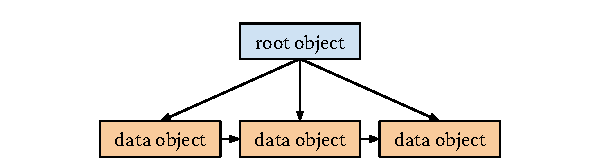
\includegraphics[width=\linewidth]{fig/objectchain1.pdf}
    \caption[Chaining objects]{Using a root object as an index to list multiple data objects that can be viewed logically as a contiguous block of data.}
    \label{fig:objchain1}
\end{SCfigure}

\begin{SCfigure}
    \centering
    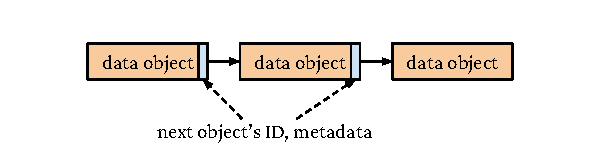
\includegraphics[width=\linewidth]{fig/objectchain2.pdf}
    \caption[Alternative object chaining]{Similar goals as in Figure~\ref{fig:objchain1}, but here we do away with the index object.}
    \label{fig:objchain2}
\end{SCfigure}
\paragraph{Chaining Objects}
The 1~GiB maximum object size may seem quite limited, but this may be because it is natural to think that they are
Twizzler's analogue to files in \unix. This is not the case---they are more similar to pages. If one wanted a
file abstraction in Twizzler, wherein the size of the file can grow largely without bound, we can simply chain multiple
objects together. Figures~\ref{fig:objchain1} and~\ref{fig:objchain2} show some possible schemes for accomplishing such
chaining, wherein we either form a linked list of objects (which would be effective for small, linear-accessed objects)
or have an index object that provides a list of data object for this ``file''. A variety of mechanisms are possible,
ranging from those depicted here, to nesting such solutions and forming an ``indirect block'' style of tracking data.
Since the minimum object's \emph{physical} size is 4~KiB, the overhead of having extra indexing objects is low.



\section{Object IDs}

We already discussed above that object IDs are 128~bits in size, but we should take a moment to discuss this choice,
along with how IDs are allocated. One aspect of our global address space we haven't discussed is coordination on IDs---that is,
when creating a new object, we must assign it an ID. Where does that ID come from?

One solution is via a centralized mechanism---some server hands out IDs when asked. The trouble here is scalability:
that centralized server will be quickly overloaded. Furthermore, the stated aim of our system is to allow devices and
nodes to act more independently to enable more concurrency. Yet a centralized solution would force them all through this
single bottleneck. Another similar solution would be a federated ID system, where we allocate ranges of IDs to a set of
centralized allocators, similar to MAC addresses. While a federated approach alleviates the problem somewhat, it still
has scalability problems and requires some out of band coordination ahead of time.

Part of the reason we selected a large ID space in the first place is to make it possible to assign IDs without
\emph{any} coordination. To ensure object ID uniqueness, we assign IDs by randomness. As long as we can ensure a high
enough chance of avoiding collision in the ID space, this method is scalable and fast.

We employ a probabilistic argument for avoiding collisions in the
object ID space. Since object IDs are generated randomly, we can model object IDs as an occupancy
problem in a space of $N = 2^{128}$ bins. Thus the probability of collision
is~\cite{motwani95}:

% TODO center equations
\begin{gather*}
    1 - e^{-
            \eqnmarkbox[NavyBlue]{m1}{m}
            (
            \eqnmarkbox[NavyBlue]{m2}{m}
            -1) / 2
            \eqnmarkbox[Orange]{n}{N}
        }
\end{gather*}
\annotatetwo[yshift=0.5em]{above}{m1}{m2}{\# of objects}
\annotate[yshift=-0.2em]{below}{n}{\# of object IDs}

% TODO: verify this math
If a system were to create millions of objects per second over the course of hundreds of years, the
probability of ID space collision is approximately 1 in $10^{7}$. However, such a system is all but
guaranteed to suffer hardware errors that flip bits\sidenote{Take DRAM bit error from cosmic rays,
    for example.} in that time frame, and so an ID space collision is dramatically more likely to be
sourced from a hardware malfunction\sidenote{This is a common comparison when considering
    probability of a randomized computer process~\cite{hollingsworth:ssr97}.}. Further, the ID space
could be expanded to 256~bits, which would dramatically reduce the chances of collision.

The reliance on randomized ID allocation is the primary reason we chose to make our object ID space
so much larger than some previous approaches~\cite{pmdk,pmdk-pointers}. Consider that if $N = 2^{64}$
bins, the probability of collision with just one billion objects is around 2\%. Increasing $m$ to
one object per person brings the collision probability up to nearly 75\%. Of course such an ID space
is usable if the ID are allocated via coordination with a centralized allocator, but if
we wish to allow object ID creation at scale, avoiding coordination is vital\sidenote{As we will
    discuss in the next chapter, some of these previous approches chose to put up with coordination and
    centralization because of the way they encoded their references. Twizzler uses a different method
    that allows ID space to be much larger.}. These alternative approaches with smaller ID spaces lead to problems when
sharing, since moving an object from one node to another requires either coordination or application-specific fixup
operations to avoid collisions.

\section{Mapping Back to Virtual Memory}


\label{sec:view}


While virtual addresses are the wrong abstraction
for data access in a data-centric system, modern hardware provides (and often requires) the use of virtual address
hardware that we can leverage for protection and isolation, adding additional ephemeral state. Often these virtual
address spaces are the only method for applications to access memory. Thus Twizzler uses virtual memory hardware to
provide a data object access mechanism to programs.

\Twizzler defines objects called ``views'', which define the current
layout of the virtual address space\sidenote{Among other things, see Chapter~\ref{ch:twizzler}.}. Twizzler
provides access to data objects by mapping them into the virtual address space
behind-the-scenes (via \libcore). The view object contains structures to define the layout of the
virtual address space which the kernel reads and uses to program the MMU accordingly.

Figure~\ref{fig:view} shows how view objects lay out the address space of any threads running inside
that particular view. View objects are manipulated by userspace and interpreted by the kernel. When
applications map objects, they update the view to specify that that object should be addressable at
a specific location. On a page-fault, the kernel reads the view and maps the object at the requested
location. The view object is laid out like a page table, where each entry in the table corresponds
to a slot in the virtual address space. Each table entry contains an object ID and requested
protection bits to further protect objects atop access control mechanisms, similar to
\texttt{PROT\_*} in \texttt{mmap}.

\begin{SCfigure}
    \centering
    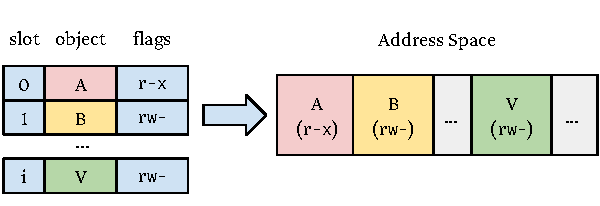
\includegraphics[width=\linewidth]{fig/view}
    \caption[Layout of a view object]{Layout of a view object. The kernel consults the view object's mapping on page-fault,
        and maps in the requested objects at the appropriate location in the virtual address space.}
    \label{fig:view}
\end{SCfigure}

When a page-fault occurs, the fault handler tries to handle the fault by either doing copy-on-write,
checking permissions, or by trying to map an object into a slot if the view object requested one.
If it cannot handle the fault, \eg due to a protection error or an empty entry in the view
object, it elevates the fault to userspace where \libcore handles it, possibly by killing the
thread, or possibly by mapping an object if the slot is ``on-demand''. This is similar to userspace
paging systems~\cite{l4,accetta:usenix86s}. When the kernel
maps an object into a slot, it updates the address space's page tables appropriately.

Note that the use of virtual memory hardware and temporary object mapping into an ephemeral space does not mean that we
aren't using a global address space. In fact, in the next section we'll discuss \emph{another} non-global address space
that we make use of. Instead, think of these address spaces as implementation quirks for specific hardware. On x86, the
use of virtual addressing is all but required---if we had other hardware and addressing designs, we would have a
different layer here for providing actual object access. Finally, applications can ignore most of the \libcore mapping
work, since they still talk about data via the object ID and offset tuple.

\section{A Logical Address Space}

The interface presented to hardware must enable interaction with a
\textit{heterogeneous memory system} and support the abstraction of an object space rather than a
collection of flat memory spaces. Unlike applications, hardware has no need for
a global address space. Rather, hardware must
have the ability to transfer large chunks of objects to, from, and around memory, access memory words, and must be able to
handle access to different \emph{types} of memory, preferably in a way that is largely transparent to
applications.

It's important to note that here when I'm talking about \emph{hardware}, I am drawing an important distinction between
the software (or firmware) running on a hardware device, and the hardware itself. The former I'm grouping in with
software in general, as in the limit, we want that software or firmware to interact with data and other applications
just as any other piece of software might. By contrast, the hardware is the substrate upon which the software runs.
Hence while software sees and interacts with a global address space, the hardware sees but wires coming out to
electrically interact with other components.


Both software and hardware must have a way of translating a
name for some piece of data into a physical address. The software's method is to rely on mapping functionality provided
by the hardware, thus kicking the can down the road. The hardware must therefore know how to translate an object ID and
offset into physical memory.
This mapping may change frequently as the OS changes allocation of physical
pages to data (\eg, to persist a piece of data).
Hardware need only know
the mappings for a short time, and need not even care about the ``canonical''
name for the object or piece of data---it simply needs to know
how to access data in memory
for a single operation. In contrast, software must have longer-term mappings, and must
be able to support data shared between threads, potentially mapped into the threads
in different places.
Our design must support appropriate abstractions for both software and hardware,
allowing software to name data while providing hardware and
the operating system with the ability to move that data into, out of, and around physical memory, preferably with
compatibility for
existing hardware functionality.

We use an additional abstraction that sits underneath the global address space---a \emph{logical address space}. The
logical address space allows hardware to address data without needing knowledge of the data's physical location. Today,
hardware must worry about emitting loads and stores to physical memory, but in a world of heterogeneous physical memory,
the location of data is likely to change overtime. Ideally, this movement will be transparent to software, with the
exception of setting policy, but for hardware, it cannot be. Requiring hardware to access a global object space through a $\langle \mathit{object},
    \mathit{offset} \rangle$ tuple is unnecessary overhead and complexity---hardware need only ever
access the ``working set'' of objects currently undergoing computation. Thus, the logical address space
maps objects within it to physical memory pages, managed by the
operating system. This solves the heterogeneity problem by allowing hardware to refer to data within
objects instead of physical addresses, whose lifetimes are much smaller than the objects, and
doesn't require hardware to emit (likely large) addresses for the global address space.

\begin{SCfigure}
    \centering
    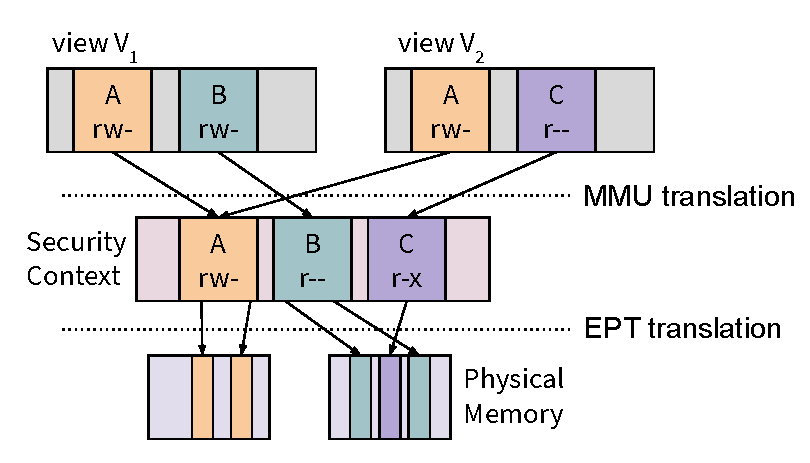
\includegraphics[width=\linewidth]{fig/2level}
    \caption[Two-level translation scheme]{Two-level translation scheme. The top level maps objects in virtual memory (defined by view
        objects) to those in object-logical space. The layout of the second level address space is managed
        by the kernel, since it is not user-facing, and the permissions are derived from a security context
        object. The second level maps to physical memory.}
    \label{fig:twolevel}
\end{SCfigure}


While SASOSes are not a viable solution to the problem of persistent pointers, they are
\emph{a} solution to implementing the logical object space.  Hardware, and the CPU, are
directly connected, reducing the cost of invalidation and coordination of an address space.
Additionally, this address space is \emph{intermediate} and hidden from programs---a virtual
address is translated to the logical object space, after which the address is translated to a
physical location (shown in Figure~\ref{fig:twolevel}) by a second address translation. The result is that all devices,
including the lower level parts of the CPU, can share a single map of current objects in the logical object space. We
implement this on current x86 hardware via a combination of the IOMMU and the Extended Page Tables, and will discuss
this in more detail and how we use it to enhance security and low level kernel implementation in Chapter~\ref{ch:twizzler}.

\begin{chconc}
    A global address space provides a way for us to organize all data, and giving all data an authoritative name via an
    object ID and an offset allows us to provide a substrate for building more complex semantics later. Importantly, the
    uniqueness of object IDs and the isolated process for generating them means that we can avoid coordination on
    organizing the global ID space. As we will see, the choices of a large ID space that needs little coordination will
    play a big part of our solution to distributed memory. But now we are left with a question: if we name data via a
    tuple of an object ID and an offset, how do we implement an actual pointer?
\end{chconc}

\chapter{Invariant References}\label{ch:invariant}

\section{Implementation}


\unedit{
    Section~\ref{sec:datacentric} discussed the needs for references that outlive ephemeral actors.
    \Twizzler provides \emph{cross-object} persistent pointers so that a pointer refers not to
    a virtual address but to an offset within an object by encoding an \texttt{object-id}:\texttt{offset}
    tuple. This enables a pointer to refer to persistent data,
    but it also allows objects to have \emph{external} pointers that refer to data in any object in the
    global object space.
    %with the same semantics as internal pointers.
    We highlight cross-object pointers' power
    and flexibility by demonstrating their ability to express inter-object relationships in Section~\ref{sec:eval}.


    To efficiently encode this tuple, we use indirection through a per-object \textit{foreign
        object table} (FOT), located at a known offset within each object. The FOT is an array of entries
    that each stores an object ID (or a name that resolves into an object ID, as we will see
    below) and flags. A cross-object pointer is stored as a 64~bit
    \texttt{FOT\_idx:offset} value, where the \texttt{FOT\_idx} is an index into the FOT\@. This provides us
    with both large offsets \emph{and} large object IDs, since the IDs are not stored within the pointer
    itself.
    If an object wishes to point to data within itself (an \emph{intra-object} pointer), it stores $0$ in
    \texttt{FOT\_idx}. When dereferencing, \Twizzler uses the \texttt{FOT\_idx} part of the
    pointer as an index into the FOT, retrieving an object ID\@.
    The combination of a FOT and a cross-object pointer logically forms
    an \texttt{object-id:offset} pair, as shown in Figure~\ref{fig:fottran}.

    Our design (discussed in prior work~\cite{bittman:hotstorage19,bittman:plos19}) differs from existing
    frameworks~\cite{corbato_introduction_1965,bensoussan:sosp69,daley:cacm68,pmdk-pointers,libpmem,Chen:micro17}
    because of the indirection. Frameworks like PMDK store entire object IDs within pointers,
    increasing pointer size and reducing flexibility by removing
    the possibility of late-binding (discussed below). Additionally, \Twizzler extends the
    namespace of data objects beyond one machine, as machine-independent data references
    are a natural consequence of cross-object pointers. Existing solutions are limited
    in this scalability. They either limit the ID space (necessary for storing IDs
    in pointers) and thus resort to complex coordination or serialization when sharing, or
    they require additional state (\eg per-process or per-machine ID tables) that must
    be shared along with the data, forcing the receiving machine to ``fix-up''
    references. Worse still, the fix-up is application-specific, since the object IDs are
    within any pointer, not in a generically known location.
    Our per-object FOT results in self-contained objects that are easier to share, thus interacting better with remote shared memory systems.

    Part of our motivation for indirecting pointers through the FOT was to allow a large ID space
    without increasing pointer size. The density of \NVM and the disaggregation of memory and
    applications means that we will be accessing data in a larger and larger address space, and it is
    vital that our abstractions allow for a large enough ID space to cover these needs. Since our IDs
    are 128~bits and our offsets need to support large objects, replacing pointers with a ``fat
    pointer'' style of just \texttt{object-id}:\texttt{offset} would mean more than doubling pointer
    size, which we found unacceptable. Other frameworks like PMDK, by contrast, increase pointer size to 128~bits for each
    pointer by encoding pointers as this tuple with 64~bit object IDs. The trade off is that our
    pointers take a little more work to translate (as they require an FOT lookup), but in return we keep
    pointers 64~bits while supporting a truly global-scale address space. Thus the overall space trade off is, for \Twizzler, no additional space overhead
    per pointer, but an added 32-byte overhead per FOT entry.
    The number of FOT entries, however, is typically much smaller than the number of
    pointers since pointers to the same external object can all use the same FOT entry. As we will see
    in Section~\ref{sec:res}, this has a dramatic benefit to performance.


    \paragraph{FOT Entries and Late-Binding.}

    The FOT entry's \texttt{flags} field has bits for read, write, and execute protections. The
    protections are \textit{requests}; \Twizzler implements separate access control on objects.
    This allows some pointers to refer to data with a read-only reference while others can be used for
    writing, reducing stray writes (a single ID can repeat in the FOT with different protections).
    The FOT entries also enable atomic updates that apply to all pointers using
    that FOT entry.
    %Additionally, the flags can contain other information, such as
    %reference counts, which can be updated atomically for all pointers using that FOT entry.

    \begin{SCfigure}[tb]
        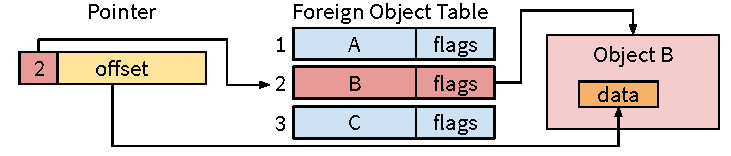
\includegraphics[width=\linewidth]{fig/ptrfot}
        \caption{Pointer translation via the FOT\@.
            The pointer and the FOT
            are both contained in the same object (not shown). An FOT entry of $0$ indicates an ``internal''
            pointer.
        }
        \label{fig:fottran}
    \end{SCfigure}

    Instead of \emph{requiring} programmers to refer to objects via IDs only, we allow
    names in FOT entries. These entries may contain a pointer to an
    in-object string table that contains a name.
    %and a function pointer that resolves the name into an
    %object ID.
    Names enable late-binding~\cite{daley:cacm68}, a
    vital aspect of systems, allowing references to objects which change over time, \eg shared library versions.
    Names are passed to a \textit{resolving} function (specified in the FOT entry).
    Allowing a program to specify how its names are resolved
    increases the flexibility of the system beyond supporting \unix paths. \Twizzler
    provides a default name resolver that uses \unix-like paths.% for ease of development of simpler applications.

    The implementation of naming is orthogonal to \Twizzler's design. We
    allow a range of name resolution methods within the system stack
    and allow objects to specify their own name resolution functions for flexibility. For example,
    objects could be organized by both a relational database and a hierarchical namer
    similar to conventional file systems. Non-hierarchical file systems
    are well studied~\cite{gifford:sosp91, ames:mss06, padioleau:usenix03, gopal:osdi99,
        parkerwood:systor14}, but these systems do not easily cooperate atop a single data space.
    Since \Twizzler uses a flat namespace as its ``native'' object naming scheme, it
    enables the required cooperation.

}


\section{Evaluation}

\unedit{
    %rewrite
    We approached these goals two ways: porting existing software (SQLite) and writing new
    software for \Twizzler. The first demonstrates both the generality of the programming environment
    (legacy software can be easily ported) and the potential performance gains to be had even for legacy
    software. The second demonstrates the true power of \Twizzler's programming model and allows us
    to explore the consequences of our design choices fully without being constrained by legacy designs.

    We built three pieces of new software: a hash-table based key-value store (KVS), a red-black tree
    data structure, and a logging daemon. Each had different characteristics and goals, and together
    they demonstrate the flexibility that \Twizzler offers in allowing simple implementation,
    nearly-free access control, and the ability to directly express complex relationships between
    objects.  Using our KVS and red-black tree code, we ported SQLite (a widely used
    SQL implementation) to \Twizzler along with a YCSB~\cite{ycsb,ycsbc} driver (a common benchmark),
    allowing us to explore \Twizzler's model in a larger, existing program that
    would let us study the performance of \Twizzler in a complex system that stores \emph{and
        processes} data. We present the performance of SQLite and our new software, along with microbenchmarks,
    in Section~\ref{sec:res}.
}

\subsection{Case Studies}

\unedit{

    \subsection{Case Study: Key-Value Store}

    %We implemented several applications and data structures to determine the effect of cross-object
    %pointers and \Twizzler's design on programming and system functionality.

    %\subsubsection*{Key-Value Store}
    \label{sec:kv}

    We implemented a multi-threaded hash-table based key-value store (KVS), called \nvkv, to
    study cross-object pointers and our late-binding of access control.
    Our KVS supports insert, lookup, and delete of values by key (both of arbitrary size), and hands
    out direct pointers to persistent data during lookup. During insert, it copies data into a data
    region before indexing the inserted key and value. We built \nvkv in multiple phases to study how
    our system handles changing requirements.

    We built \nvkv in roughly 250 lines of C\@. Handing
    out direct pointers into data was trivial to implement with cross-object pointers, requiring
    only a call to \texttt{ptr\_lea} during lookup. The initial implementation maintains two
    objects, one for data and one for the index.  The complexity typically involved when storing both
    index and data in a single, flat file is not justified in a programming
    model where we can express inter-object relationships directly at
    near-zero cost in complexity or performance. In our case, a pointer from the index object
    to the data object (such as an entry in the hash table) can be written with a single call to
    \texttt{ptr\_store}.
    %to translate the pointer from an offset into the data object into a cross-object
    %pointer for storage in the index. 
    This, combined with the simple requirements for an in-memory \NVM KVS,
    resulted in a small implementation that was nonetheless a
    usable KVS.

    \begin{SCfigure}
        \centering
        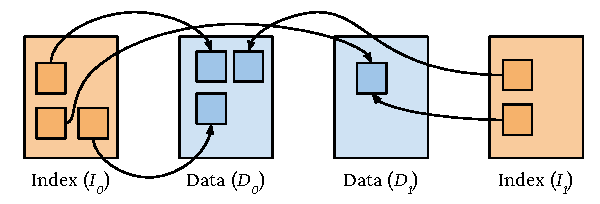
\includegraphics[width=\linewidth]{fig/twzkv}
        \caption{Cross-object pointers in \nvkv. The index object contains pointers to keys and values,
            which can reside in any data object. We also support multiple indexes to enable additional
            indexing strategies and access control on discovery. Because \Twizzler provides native support
            for cross-object pointers, this kind of construction is no more complex than keeping all keys
            and data within a single object.}
        \label{fig:twzkv}
    \end{SCfigure}




    \paragraph{Extending Requirements.}

    Next, we added functionality to protect values with access control. We wanted to
    keep handing out direct pointers to data during lookup and to
    keep \nvkv a library (as opposed to a service). Meeting these goals on an
    existing system would be difficult without adding significant
    complexity, such as reimplementing a lot of \Twizzler's pointer framework or implementing manual,
    redundant access control.

    In \Twizzler, implementing access control in \nvkv involved having the index refer to data in
    multiple data objects, assigning those objects different access rights, and allocating from
    those objects depending on desired access rights. We were
    able to implement this while preserving the original code due to the
    transparent nature of \Twizzler's cross-object pointers. Now, when inserting, the application
    indicates the data object into which to copy the data, as shown in Figure~\ref{fig:twzkv}.

    By supporting multiple data objects, \nvkv can leverage the OS's access control,
    minimizing complexity. Unrestricted data can go in $D_0$ (Figure~\ref{fig:twzkv}),
    whereas restricted data can go in $D_1$. Since each object has distinct
    access control, a user can set the objects' access rights, then decide
    where to insert data according to policy. The indexes point to the
    correct locations regardless of the access restrictions of the data objects, and \nvkv still hands
    out direct pointers, but a user that is restricted from accessing data in $D_1$ will not
    be able to dereference the pointer. A further extension is to support secondary indices, as shown in
    Figure~\ref{fig:twzkv}, enabling alternative lookup methods and limiting data discovery
    with index object access control. This extension is easy to implement on \Twizzler.
    %increasing our implementation's complexity only a small amount.

    \paragraph{Comparison to \unix Implementation.} To compare with existing techniques, we built a
    similar KVS using only \unix features (called \unixkv). It also separates index and data, but it
    must manually compute and construct pointers, requiring a significant amount of programmer time to
    get right.
    Supporting multiple data objects was complex in \unixkv, because we had to store and process file
    paths in the index and store references to paths for pointers, increasing overhead and code
    complexity by 36\%---a lot for an implementation with relatively few pointers---just to reimplement
    \Twizzler's support. The extra complexity also included code to manually open, map, and
    grow files, much of which \Twizzler handles internally. Development time was extended by
    bugs that were not present when developing \nvkv, due to the manual pointer processing.  While \nvkv
    gains transparent access control, \unixkv does not due to the lack of
    on-demand object mapping and late-binding of security. Instead, \unixkv needs to know object permissions before
    mapping,
    a restriction that limits the ability to reuse OS access control, something that
    \nvkv could leverage through late-binding on security (\S~\ref{sec:sec})\footnote{\unixkv could trap segmentation faults to do this, but that would be
        application-specific, difficult, and would reimplement \Twizzler functionality.}. Other frameworks like PMDK
    that do not integrate access control and late-binding into their models have similar
    limitations.


    %% TODO RUST SYNTAX
    \subsection{Case Study: Red-Black Tree}
    To evaluate the process of writing persistent, ``pointer-heavy'' data
    structures,
    we implemented a red-black tree in C using normal pointers (\ramrbt)
    in 100 lines of code,
    and evolved it for persistent memory in two ways: manually writing
    base+offset style pointers, as current systems require (\unixrbt),
    and using \Twizzler (\nvrbt).
    Porting existing data structure code to persistent memory
    will be common during the adoption of \NVM, and much of the complexity therein
    comes from dealing with persisting virtual addresses~\cite{virendra:hotstorage17}.

    In developing \unixrbt, we found 83 locations where we had to perform pointer arithmetic for
    converting between persistent and virtual addresses.  Consider an expression such as
    \texttt{root->left->right = foo}. Inserting calls to translate this directly results in
    \texttt{L(L(root)->left)->right = C(foo)}, where \texttt{L} converts to a virtual address and
    \texttt{C} converts back, which is heavily obfuscated and took more development time than writing
    \ramrbt in the first place due to debugging.

    We built \nvrbt like \unixrbt, annotating pointer stores and
    dereferences. However, \unixrbt used an application-specific solution for pointer
    management; if other applications wanted to use the data structures created by \unixrbt, they would
    have to know the implementation details of the pointer system (or share the implementation, thus
    reimplementing much of \Twizzler's library).  Additionally, due to \Twizzler enabling improved
    system-wide support for cross-object pointers, these transformations can be made automatic through
    compiler and linker support.

    Unlike \nvrbt, \unixrbt's tree is limited to a single persistent
    object; a limitation that prevents the tree from growing arbitrarily, does not
    allow it to directly encode references to data outside the tree object, and does
    not gain it the benefits of cross-object data references that were discussed
    above for \nvkv. Adding support for this to \unixrbt would require modifying the
    core data structures to include paths and significantly altering the code,
    increasing its length by at least a factor of 2, whereas \nvrbt gets this
    functionality for free.

    Another advantage of \nvrbt is reduced support code compared to \unixrbt; \unixrbt needed
    code to manage and grow files and mappings, while we implemented \nvrbt as simple data structure code
    with \Twizzler managing that complexity. The additional error handling code and pointer
    validity checks in \unixrbt (handled automatically in \Twizzler) increased development time
    and implementation complexity.


    \subsection{Porting SQLite}

    We ported SQLite to \Twizzler to demonstrate our support for existing software and to evaluate the
    performance of a SQLite backend designed for \Twizzler. We used
    our POSIX support framework, a combination of \texttt{musl} and our library
    \texttt{twix}, to support much of SQLite's POSIX use.
    We took a modified version of SQLite called SQLightning that replaced
    SQLite's storage backend with a memory-mapped KVS called LMDB~\cite{lmdb}.
    We chose this port
    because LMDB is implemented with \texttt{mmap}'d files as the primary access method and hands out
    direct pointers to data as one would expect from an effectively designed \NVM KVS\footnote{These
        are not persistent pointers, however, unlike \Twizzler's.}.
    Since LMDB's SQLightning port already replaces the storage backend
    with calls to
    LMDB, we ported SQLite to \Twizzler by taking our KVS and red-black tree code and implementing
    enough of the LMDB interface for SQLite to run using \Twizzler as a backend.
    Outside of the
    B-tree source file few changes were needed for
    SQLite to run on \Twizzler. We further ported our modified SQLite backend to PMDK to compare
    directly with a commonly used \NVM programming library that supports persistent pointers.

    We also ported a C++ YCSB driver~\cite{ycsbc}, which required porting the C++ standard template
    library (STL). Since we had already ported a standard C library, the C++ STL was easily ported,
    demonstrating the ease of porting software to \Twizzler.
    We have also ported some existing \unix utilities (such as \texttt{bash} and
    \texttt{busybox}), which largely require only recompiling to run on \Twizzler. Of
    course, to gain \emph{all} of the benefits of \Twizzler, programs will be need to be
    written with \NVM in mind (but this is true regardless of the target OS).
    %Our POSIX shim library provides emulated Linux system call support to \texttt{musl},
    %implemented in userspace, such that C programs need only be recompiled.

    Our implementation of the LMDB interface
    corroborated our experience from the KVS case study: much of the complexity in storage interfaces
    and implementations comes from the separation between storage and memory. This has been
    studied before (as we will elucidate in Section~\ref{sec:relwork}), but the advent of \NVM changes the game
    significantly by allowing programmers to think directly via in-memory data structures. The result is
    that interfaces like cursors in a KVS become redundant. We implemented to this interface
    for LMDB, but the functions were largely wrappers around storing a pointer
    to a B-tree node and traversing the tree directly without separate loads and copies. The result was
    an extremely simple implementation (500 LoC) that still met the required interface. Future software
    for \NVM can use \Twizzler's programming model to more effectively write software
    that eschews the need for complexity forced by the two-tier storage hierarchy.

}

\unedit{

    \subsection{Discussion}

    Although these implementations were simple, they represent the applications
    and data structures we expect in a data-centric system. Persistent pointers
    we can directly use in our programming languages make computing over persistent
    data almost transparent, allowing simple implementations that are nevertheless
    easy to evolve as requirements change.
    %The model does not restrict systems
    %applications to shared-memory style interaction; as we saw with \twzlogd,
    %applications can use stream-like, message-passing, and synchronous calling
    %abstractions atop \Twizzler's programming model. These abstractions were
    %similarly easy to build and use, reflecting the simplicity of the data model in
    %\Twizzler.

    Not only does \nvkv have strong support for access control, it enables
    concurrent use of databases via cross-object pointers. Applications can load indexes
    for multiple databases without needing to worry about address space layout and
    without writing complex pointer management code that would be required by an
    implementation using \texttt{mmap}.
    We were able to provide access
    control without a single line of code in \nvkv dedicated to checking or enforcing
    access rights. Instead, we relied on \Twizzler's built-in access control, something not possible with other
    frameworks that do not support late-binding of access rights and do not consider
    security as part of their programming model. \Twizzler thus removes
    the need for applications to enforce and implement their own access control, which
    increases the security of the system by divesting programmers from
    the responsibility of getting the enforcement right.
    Similar functionality for current
    systems would traditionally require separation of the library and application
    into a client-server model, but that additional overhead is unneeded here and
    inappropriate on a persistent memory system.

    Although \nvrbt and \nvkv had different densities of pointer operations, \nvrbt being
    ``pointer-heavy'' and \nvkv being ``pointer-light'', \Twizzler improved the complexity of both
    over manual implementation and improved flexibility over existing persistent
    pointer methods. Using a system-wide standardized approach to
    pointer translations not only enables better compiler and hardware support, but it also improves
    interoperability; because they share a common framework, \nvkv could use the red-black tree code and data with ease, and even interact with
    the SQLite database even though they were written separately without that goal in mind.
    %\emph{because} they share a common framework.
    The position-independence afforded by this model
    enables both composability and concurrency, while also simplifying programming on persistent data to
    a natural expression of data structures.

}

\subsection{Storage Overhead}


\begin{SCfigure}[t]
    \centering
    \includegraphics{genfig/fotoverhead}
    \caption{TODO}
    \label{fig:fotoverhead}
\end{SCfigure}



\subsection{Performance}

\unedit{\label{sec:res}

    %\dab{New experiments we can run!!! Time a linux syscall vs. a twix syscall vs. a twizzler syscall.
    %I have some old data on number of syscalls made by sqlite, but it's from FreeBSD Twizzler. That
    %said, it's unlikely to have changed.}


    Our evaluation's primary focus is on the benefits of the programming model, showing new
    functionality with reduced complexity at an acceptable overhead. Nevertheless, there are many
    cases
    %focused not on performance increase---the
    %benefits of \Twizzler are primarily the programming model---but instead on
    %demonstrating acceptable performance with new functionality and reduced complexity. However, there are many cases
    where we see significant improvement (such as SQLite)
    because the programming model has less overhead, and our pointer design is space
    efficient and fast to translate.
    %In some cases, this is due
    %to fewer system calls, but performance gains also arise elsewhere, as our experiments against
    %SQLightning show.


    We measured the performance of our KVS and red-black tree, performed
    microbenchmarks, and evaluated the \Twizzler port of
    SQLite against Linux (Ubuntu 19.10) instances of SQLite, SQLightning, and our port of SQLite
    to PMDK\@. Tests ran on an
    Intel Xeon Gold 5218 CPU running at 2.30 GHz with 192 GB of DRAM and 128 GB of Intel
    Persistent DIMMs.
    We compiled all tests against the \texttt{musl} C library instead of
    \texttt{glibc} because \Twizzler uses \texttt{musl} to support \unix programs.

    All Linux tests used the NOVA filesystem~\cite{Xu:nova} (a filesystem
    optimized for \NVM) on the NVDIMMs, mounted in DAX mode. This enabled direct access to the
    persistent memory without a page-cache interposing on accesses.
    %The use of persistent memory allows
    %us to account for differences in behavior of the NVDIMMs compared to DRAM.

    \subsection{Microbenchmarks}

    Table~\ref{tbl:res} shows common \Twizzler functions' latencies, including pointer
    translation (loading and storing) and mapping overhead.
    The overhead shown for resolving pointers does not
    include dereferencing the final result, since that is required regardless of how a pointer is
    resolved. The first row shows the latency for resolving pointers to objects the first time.
    \Twizzler makes a further optimization by
    caching the results of translations for a given FOT entry. Each successive
    time that FOT entry is used to resolve a pointer, the result of the original translation is returned
    immediately, improving the latency as shown on the ``cached'' row of Table~\ref{tbl:res}. Note that
    the low latency of these results is expected; the performance critical case of these functions' use
    is repeated calls, and since these operations are simple, they fit within the processor cache.

    \Twizzler translates intra-object pointers by first
    checking if the pointer is internal and, if so, adding the object's base
    address to it---the same operation required for application-specific
    persistent pointers. The expanded programming model offered by \Twizzler
    %and the improved I/O
    %performance
    makes this overhead minor relative to the high costs for persistent data access on
    current systems, which have high-latency for equivalent operations.
    %\textcolor{blue}{While existing frameworks could
    %have similar or slightly faster pointer resolution times, they lack the flexibility our model
    %provides (see Section~\ref{sec:invariant_pointers}) and thus a performance comparison is not as
    %eluciating.}
    %, and the additional work is dwarfed by transfer latencies from memory.

    \begin{SCtable}
        \centering
        \caption{Latency of common \Twizzler operations, including pointer loading and storing, and object
            mapping.
        }
        \begin{minipage}{\linewidth}
            \centering
            \begin{tabular}{c | S[table-format=7.1]@{\,\,\( \pm \)\hspace{-5mm}} S[table-format=0.1]}
                \textbf{Pointer Resolution Action} &
                \multicolumn{2}{c}{\textbf{Average Latency (ns)}} \\
                \hline
                %First-time translation  & 26.9 & 0.1 \\
                %Object already mapped & 5.8 & 0.1      \\
                Uncached FOT translation           & 27.9 & 0.1   \\
                Cached FOT translation             & 3.2  & 0.1   \\
                Intra-object translation           & 0.4  & 0.1   \\
                Inter-object pointer store         & 17.2 & 0.6   \\
                Intra-object pointer store         & 2.3  & 0.1   \\
                Mapping object overhead            & 49.4 & 0.2
            \end{tabular}
        \end{minipage}
        \label{tbl:res}
    \end{SCtable}

    The pointer store operations shown in Table~\ref{tbl:res} measure the latency of the
    \texttt{ptr\_store} operation that is used to construct persistent data references in \Twizzler.
    While these operations are less common than pointer loads, their overhead directly affects
    applications that perform many updates to data structures.
    The most common pointer store operation applications perform is internal (intra-object) pointer stores, in which the
    overhead is minimal. Pointer store operations for external (inter-object) references have slightly
    more overhead, since they need to perform an FOT scan to allow FOT entry reuse.



    We compared our pointer translation to \unix functions.
    Resolving an external pointer with an ID corresponds roughly
    to a call to \texttt{open("id")}, which has a latency of $1036 \pm 15$ ns.
    The comparison is not exact, of course; the pointer resolution
    also maps objects, and the call to \texttt{open} must handle file system
    semantics. However, the direct-access nature of \NVM results in pointer translation
    achieving the same goal as opening a file does today. The pointer operations in \Twizzler accomplish
    much of the same functionality as the heavier-weight I/O system calls on \unix with more utility and
    less overhead.

    %The overhead of system calls is enormous compared to the pointer
    %translation operations of \Twizzler.
    %, although both achieve the result of
    %persistent data access.
    A more direct comparison is object mapping, which has
    low latency compared to \texttt{mmap} ($658.7 \pm 12.7$ ns---a $13.3\times$ speedup) though the two have similar
    functionality. Since mapping occurs entirely
    in userspace, cache pollution is reduced.
    While both \texttt{mmap} and \Twizzler's mapping require
    page-faults to occur before the data is actually mapped,
    this overhead is similar in \Twizzler and \unix, and so is not
    shown.


    %% TODO maybe cut this
    %It is important to keep in context the latency of these operations, many of which 
    %replace relatively heavy \unix operations in functionality in \Twizzler's memory-access
    %model. Most of the equivalent \unix operations require
    %at least one system call, which is untenable for low-latency persistent
    %storage.
    %The mitigations for both Spectre~\cite{spectre} and
    %Meltdown~\cite{meltdown} further motivate reducing system calls, especially with
    %NVM, since they further increase system call latency.


    \subsection{SQLite}

    We ran four variants of SQLite, three on Linux and one on \Twizzler, and compared their performance: ``SQL-Native'' (unmodified SQLite),
    ``SQL-LMDB'' (SQLite using LMDB as the storage backend), ``SQL-PMDK'' (SQLite using
    our red-black tree on PMDK),
    and ``SQL-\Twizzler'' (our port of SQLite running on \Twizzler). SQL-Native was run in \texttt{mmap} mode so that both it
    and SQL-LMDB used \texttt{mmap} to access data.
    We ran each on the same hardware and normalized the results.
    %All were run on the same
    %hardware, and results were normalized.
    %Because the \Twizzler port of SQLite was lacking in full transactional
    %support\footnote{Transaction support is no more difficult in \Twizzler, but as it is not germane, it
    %	was excluded from the study.},
    %we ran experiments with SQLite in read-uncommitted mode. Furthermore, we
    %ran SQL-LMDB and SQL-Native with the database on a ramdisk to remove the overhead of disk
    %I/O and filesystems as much as possible.
    %To get the most performance out of these two variants, we also ran them with
    %asynchronous writes enabled (allowing SQLite to continue after updates without a call to
    %\texttt{fsync} or \texttt{msync}).
    %We normalized results to better show comparisons.
    %rather than raw
    %values.

    Figure~\ref{fig:ycsb} shows the three variants' throughput under standard YCSB
    workloads. The performance improvement of the LMDB and \Twizzler variants over SQL-Native is
    likely due to handing SQLite direct pointers to data. However, in the \Twizzler
    case we get an additional benefit of operating on data structures directly while LMDB has an
    abstraction cost.

    \begin{SCfigure}[t]
        \centering
        \includegraphics{genfig/ycsb}
        \caption{YCSB throughput, normalized (higher is better). \Twizzler outperforms all other
            variants in all tests.}
        \label{fig:ycsb}
    \end{SCfigure}

    Figure~\ref{fig:qlat} shows the latency of queries on a one million row table.
    This is common data processing---loading and then
    examining data in a variety of ways.
    %The transaction overhead is minimal, since the
    %measurements are done on read-only operations.
    We measured the performance
    of calculating the mean and median, sorting rows, finding a specific row,
    building an index, and probing the index. SQL-\Twizzler had similar performance to SQL-LMDB and
    SQL-Native despite comparing its extremely simple storage backend to optimized B-tree
    backends (that benefit from scan operations). As a more direct comparison,
    SQL-\Twizzler significantly out-performed SQL-PMDK in most tests. PMDK's pointer operations are
    more expensive than \Twizzler's, requiring up to two hash table lookups per
    translation~\cite{pmdk-pointers}. Additionally, PMDK's
    pointers are 128~bits, while \Twizzler does not increase pointer size. Increased
    pointer size results in significantly worse cache performance, especially in a pointer-heavy data
    structure like a persistent red-black tree.


    %SQL-\Twizzler out-performed SQLite and SQL-LMDB in
    %every test. The building-index test did not see a dramatic performance improvement, but this largely
    %involved building a volatile in-memory data structure, and thus largely avoided touching persistent memory.

    \begin{SCfigure}[t]
        \centering
        \includegraphics{genfig/qlat}
        \caption{Query latency, normalized (lower is better). \Twizzler maintains a similar level of
            performance with the native and LMDB variants, despite comparing \Twizzler's simplistic
            red-black tree index
            implementation with highly optimized B-trees. \Twizzler also significantly outperforms PMDK
            despite sharing a similar implementation for the index structures.}
        \label{fig:qlat}
    \end{SCfigure}


    \subsection{Key Value Store}
    \label{sec:kvperf}

    We compared \nvkv to \unixkv
    by inserting one
    million distinct key-value pairs, followed by looking up each in-order. The inserted items were 32-bit
    keys and 32-bit values, chosen to reduce the overhead of data copying since we were focusing on
    pointer translation overhead.
    %For similar reasons, we \texttt{memset} the index to zero (to avoid
    %page-fault routines clouding the overhead of pointer translation), and we set the initial hash-table
    %size to avoid expansion (since expansion code is not affected by pointer translations).
    Both were
    compared under two modes, single-data-object and multiple-data-objects. Both KVSes translated
    between virtual and persistent addresses when storing and retrieving data, but for
    multiple-data-objects, we allow for storing the data in an arbitrary object.
    %Finally, we compared to \texttt{clang}'s \texttt{std::unordered\_map} for a baseline, even though
    %\texttt{unordered\_map} does not store data in a separate object and uses virtual addresses instead
    %of persistent pointers.

    Figure~\ref{fig:kvlat} shows the latency of lookup and insert, demonstrating
    that not only is the memory-based index and data object
    structure that can hand out direct data pointers sufficiently low latency to
    take advantage of \NVM,
    %(by our measurement, we are 36$\times$ and 45$\times$
    %faster than Berkeley DB on insert and lookup, respectively),
    but the additional overhead of cross-object
    pointers is minimal.
    %When using a single data object, the overhead is reduced
    %because the system can optimize pointer translations to 2 bitwise operations.
    Compared to \unixkv, \nvkv has minimal overhead in the single-object case, and improves lookup
    performance in the multiple-object case. The minor overhead in other cases comes with improved flexibility,
    simplicity, and access control support (\unixkv does not support access control).
    %Compared to \unixkv, \nvkv improves performance when multiple data objects are supported,
    %has significantly
    %simpler code, and supports access control mechanisms (which \unixkv does not).
    %When using single data objects, \unixkv avoids some of the overhead at the cost of flexiblity.
    %The difference in latency on insert between the KV stores and
    %\texttt{unordered\_map} can be explained by
    %different choices in hashing
    %algorithms,
    %lack of support for persisting the index and data.%, but that the additional overhead was small.
    %, and different
    %optimization levels stemming from code maturity.
    Finally,
    multithreaded access on \nvkv and \unixkv did not improve performance;
    despite the pointer translations, they ran at memory bandwidth (for \NVM).
    %It is important to note that this performance is achieved with stright-forward
    %code using \Twizzler's programming model, while providing the features of a
    %usable KV store. Additionally, access control is provided at little to no
    %additional cost in the implementation---there is no explicit code doing access
    %control checks, instead all access control is handled by the OS
    %during mapping, followed by being handled by the memory system.

    \begin{SCfigure}[t]
        \centering
        \includegraphics{genfig/kvs}
        \caption{Latency of insert and lookup in \nvkv and \unixkv.
            An ``(m)'' indicates
            support for multiple data objects. Both \unixkv and \nvkv have similar latencies.}
        \label{fig:kvlat}
    \end{SCfigure}




    \subsection{Red-Black Tree} We measured the latency of insert and lookup of 1 million 32-bit
    integers on both \unixrbt and \nvrbt. The insert and lookup latency of \nvrbt was $528 \pm 3$ ns
    and $251.8 \pm 0.5$ ns, while insert and lookup latency of \unixrbt was $515 \pm 2$ ns
    and $213 \pm 1$ ns.
    %The lookup overhead of \nvrbt arises because it does not support cross-object trees, while the
    %insert overhead of \unixrbt arises due to the management of the persistent file that is unnecessary
    %in \Twizzler.
    The modest overhead comes with significantly improved flexibility, as \unixrbt does not support
    cross-object trees, and less support code (\unixrbt manually implements mapping and pointer
    translations). Note that even though there is lookup overhead in
    \nvrbt, this overhead did not predict the results of a larger program---the SQL-\Twizzler port used
    this red-black tree, and saw performance benefits over block-based implementations.

    %we still see a performance benefit in a larger application---the SQL-\Twizzler code used
    %this red-black tree internally, and saw performance benefits during queries that were not predicted
    %by this benchmark.
}

\chapter{Twizzler: An Implementation}\label{ch:twizzler}

\section{Objects}

\unedit{
    The kernel provides services for object management, such as creating and deleting objects.
    Objects are created by the \texttt{create} system call, which
    returns an object ID\@. A program may also optionally provide an existing object ID to the
    \texttt{create} call, stating that the new object should be a copy of the existing one, for which
    \Twizzler uses copy-on-write. The new ID is a number that
    is unlikely to collide with existing IDs in the 128~bit ID space, and can be assigned using a technique
    that supports this requirement (random, hashing, \emph{etc}.).
    Some forms of ID assignment support a form of access
    control: a program can only access an object whose ID it knows. \Twizzler provides
    object naming as well, discussed in Section~\ref{sec:invariant_pointers}.

    Objects may be be deleted via the \texttt{delete} system call.
    %, however deletion is not immediate.
    Like \unix's \texttt{unlink}, objects are reference counted, where a reference refers to a mapping
    in an address space. Once the reference count reaches zero, the object may be deleted. During
    deletion, an object may be optionally marked as ``hidden'', causing new mapping requests for this
    object to fail.
}

\subsection{Creation}

\subsection{Deletion}

\section{Dealing with Ephemera}

\subsection{Threads}

\unedit{\Twizzler provides a set of threading primitives for applications. Threads in \Twizzler are always
    attached to a view and one or more security contexts. Threads may communicate with each other using
    shared memory and can signal each other with a system call.
    Since everything in \Twizzler is an object, each thread has a state object associated
    with it. Signals can be raised assuming the raiser has appropriate permissions on the state object,
    and the state object contains information about the thread.

    A key primitive in \Twizzler is the \texttt{thread-sync} system call. This call operates similar to
    \texttt{futex(2)} on Linux, except that it supports waiting on and waking up a number of different
    words of memory simultaneously. Multi-word thread-sync is necessary to support
    \texttt{select(2)}-like or \texttt{poll(2)}-like operations in a system where all data access is
    done with memory semantics. \Twizzler's standard library exposes an API for event handling that uses
    multi-world thread-sync, where objects may expose a set of ``events'' that can be triggered and waited for. This is
    used in numerous places to implement event handling for multiple communications streams implemented
    in objects.
}

\subsection{Program Instancing}


\unedit{
    \subsubsection{Ephemeral State Management with Views}
    \label{sec:view}
    \iffalse
        \dab{What we could do here is reframe this section and rename it. Sure, virtual addresses are needed, and it's how
            we map things. But there's a much more fundamental thing that we are doing here. We're providing a
            mechanism to mesh together ephemeral "moments of computation" (threads) with persistent data. We can
            add a figure here that's \texttt{threads (computation)---views (ephemeral state
                mapping)---persistent data} or something. The question is, is this something that we would want to
            include in a future publication?}
    \fi

    Despite \Twizzler's focus on persistent data, many components of our hardware and applications are
    built around ephemeral constructs. For example, threads are ephemeral ``moments of computation''
    that act on persistent data, while the programs that they execute often expect some ephemeral
    private data (\eg the data segment and the stack). While virtual addresses are the wrong abstraction
    for persistent data access, modern hardware provides (and often requires) the use of virtual address
    hardware that we can leverage for protection and isolation, adding additional ephemeral state.

    \Twizzler defines objects called ``views'', which coalesce the state
    and context necessary to support ephemeral constructs like threads and application instances into
    \Twizzler objects. A significant part of that state is ephemeral virtual address mappings; \Twizzler
    provides access to persistent objects by mapping them into the virtual address space
    behind-the-scenes (via \libcore). The view object contains structures to define the layout of the
    virtual address space which the kernel reads and uses to program the MMU accordingly. Figure~\ref{fig:view2} shows how
    views ``mesh'' ephemeral threads with persistent data by providing them a context to operate in.
    Since view objects are normal \Twizzler objects, they can be persisted, allowing
    us to recover application state after power cycles.

    \begin{figure}
        \centering
        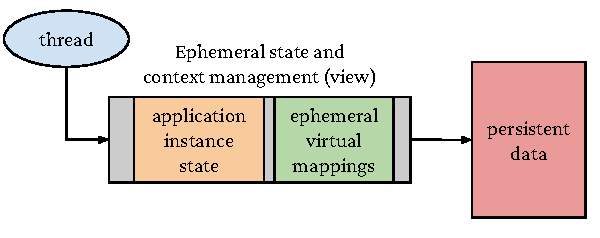
\includegraphics[width=4in]{fig/view2}
        \caption{View objects in \Twizzler. Views manage ephemeral constructs and state, giving threads
            the necessary context to execute and access persistent data.}
        \label{fig:view2}
    \end{figure}


    By coalescing this ephemeral state
    into an object, we make it possible for applications to manage it directly with minimal kernel
    involvement. Avoiding the kernel is natural---all data access already does this in \Twizzler, so
    adding a separate kernel API to manage this state would add complexity---and reduces the number of
    system calls needed when mapping objects. Additionally, avoiding the kernel necessitates an
    increased address space management responsibility for userspace. For example, executable loading
    and mapping is largely handled without the kernel.



    \iffalse
        Although virtual addresses are the wrong abstraction to use for persistent
        data access, we do leverage virtual address hardware in modern processors for isolation and
        protection.
        \Twizzler provides access to persistent objects by mapping
        them into the virtual address space behind-the-scenes (via \libcore).
        %; applications need not operate on this level of abstraction directly).
        This generates many mapping operations to access persistent data, so requiring system calls would be
        costly. Additionally, our kernel avoidance necessitates an increased address space management
        responsibility for userspace. For example, executable loading and mapping is handled largely
        without the kernel.
        %, and modern software frameworks may
        %map data into address spaces frequently~\cite{2016posix}. Requiring system calls would
        %be costly, especially when we are trying to avoid kernel boundary crossings.

        To support userspace manipulation of address spaces,
        the kernel and userspace share an object (called a ``view'') that
        defines an address space layout. The view is just a normal
        object, and so standard access control mechanisms apply to enforce isolation.
        When applications map objects into their address space, they update the view to specify
        that a particular object should be addressable at a specific location.
        The kernel then reads the object and determines the
        requested layout of the virtual address space. The view object is laid out like a page-table (shown
        in Figure~\ref{fig:view}), where
        each entry in the table corresponds to a slot in the virtual address space.
        Each table entry contains an object ID and read, write, and execute protection bits to further
        protect object access (like \texttt{PROT\_*} in \texttt{mmap}).
    \fi

    Figure~\ref{fig:view} shows how view objects lay out the address space of any threads running inside
    that particular view. View objects are manipulated by userspace and interpreted by the kernel. When
    applications map objects, they update the view to specify that that object should be addressable at
    a specific location. On a page-fault, the kernel reads the view and maps the object at the requested
    location. The view object is laid out like a page-table, where each entry in the table corresponds
    to a slot in the virtual address space. Each table entry contains an object ID and requested
    protection bits to further protect objects atop access control mechanisms (similar to
    \texttt{PROT\_*} in \texttt{mmap}).

    \begin{figure}
        \centering
        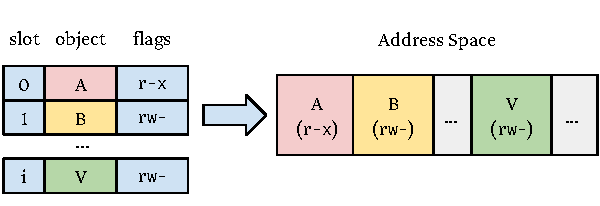
\includegraphics[width=3.5in]{fig/view}
        \caption{Layout of a view object. The kernel consults the view object's mapping on page-fault,
            and maps in the requested objects at the appropriate location in the virtual address space.}
        \label{fig:view}
    \end{figure}

    %When a fault occurs, the kernel checks if the faulting thread is a \Twizzler thread, and if so,
    %diverts it to a different fault handler.  The new
    When a page-fault occurs, the fault handler tries to handle the fault by either doing copy-on-write,
    checking permissions, or by trying to map an object into a slot if the view object requested one.
    If it cannot handle the fault (due to a protection error or an empty entry in the view
    object), it elevates the fault to userspace where \libcore handles it, possibly by killing the
    thread, or possibly by mapping an object if the slot is ``on-demand''. This is similar to userspace
    paging systems~\cite{l4,accetta:usenix86s}. When the kernel
    maps an object into a slot, it updates the address space's page-tables appropriately.

    Applications can add objects to a view with the \texttt{view\_set} function. The caller specifies a
    target object and a set of protections (see \S~\ref{sec:invariant_pointers}), and a slot in which to
    map the object. However, applications rarely invoke this function directly---instead,
    \texttt{libtwz} provides a higher-level API to allow applications to operate above the level of
    manually mapping objects. The standard library also provides access to other utility functions for
    views (such as querying state, creating new views, and copying views). These functions, by default,
    operate on a thread's current view, but they may also optionally operate on any other view object,
    which allows \Twizzler to implement operations with semantics similar to \texttt{fork} and \texttt{execve}.

    When threads add entries to a view object they need not inform the kernel---when
    a fault occurs, the kernel will read the entry as needed. However, when \emph{changing} or
    \emph{deleting} an entry, threads must inform the kernel so it can update existing page table entries.
    We provide two system calls for views. The \texttt{become} system call allows a thread to
    change to a new view, which might be used to execute a new program or jump across programs to, for
    example, accomplish a protected task. \Twizzler's access control system prevents this from happening
    arbitrarily. The second system call is \texttt{invalidate\_view}, which lets a thread inform the
    kernel of changed or deleted entries.

    View objects not only reduce kernel boundary crossings, but they also improve the resumability of
    the system. After a power cycle, the OS now has information on which objects were mapped and where,
    improving the ability of threads to pick up where they left off. Additionally, view objects
    facilitate the sharing of address spaces between threads, since they can both synchronize on
    modifying a given view object and need not duplicate information. Note that the particular contents
    of a view object are system-specific. On virtual memory systems, one of their jobs is to manage
    ephemeral virtual mappings, while on other architectures their jobs may be to manage, \eg, segment
    tables. However, in all cases, views provide a mechanism for managing ephemeral state while
    providing enough context for threads to execute.
}



\unedit{
    \paragraph{Pointer Translation.}

    Current processors provide only a virtual memory abstraction, so applications must do some
    extra work to dereference a pointer, \emph{translating} a pointer from its persistent form into a
    virtual address. This does not affect the
    \emph{stored} pointer, which is still persistent and independent of any translation or address
    space. Thus multiple applications, possibly with different address space layouts, can translate the
    same pointer at the same time without coordination.

    Pointer translation occurs with the help of two \libcore functions: \texttt{ptr\_lea}
    (load effective address) and \texttt{ptr\_store}. When a program dereferences a pointer, it first
    calls \texttt{ptr\_lea}. The pointer is resolved into an
    object-ID and offset pair through a lookup in the FOT, after which \libcore determines if the
    referenced object is already mapped (by maintaining per-view metadata). If not, it picks an empty
    slot in the view and maps the object there (a cheap operation that does not invoke the kernel). Once mapped,
    \libcore combines the object's temporary virtual base address with the offset, and
    returns the new pointer. The \texttt{ptr\_store} function does the opposite of
    \texttt{ptr\_lea}---it turns a virtual pointer into a persistent one. While these are done manually
    in our implementation, we plan to implement compiler support to emit these calls automatically.


    FOT management is handled by \libcore.
    While a lookup in the FOT is a simple array-indexing operation, a
    store may require adding to the FOT\@. To avoid duplicate entries, \libcore walks
    the FOT looking for a compatible entry.
    If one is not found, it atomically reserves a new entry and fills it (flushing cache-lines to
    persist it) before storing the pointer. The \texttt{ptr\_store} operation is less
    common than \texttt{ptr\_load}, and in the future we may include additional caching
    metadata that would speed-up the FOT walk (such as storing recent IDs).


    Translating pointers has a small overhead
    (\S~\ref{sec:res}) and the result can be cached. \Twizzler
    improves performance via a per-object cache of prior translations.
    %to speed up external
    %references.
    The common case, intra-object pointers, does not require an external
    lookup and is implemented as a simple bitwise-or operation.
    \iffalse
        \paragraph{Persistent and Volatile Pointers}
        \dab{THIS IS ALL NEW}

        Note that \Twizzler does not attempt to limit the creation of pointers between volatile and
        persistent data. This is an example of ongoing \NVM research that \Twizzler does not want to
        prematurely limit. However, we expect that this is the right decision regardless, as the goal of the
        OS is to provide a framework for higher-level abstraction, not to prescribe limitations that could
        be better handled at the language level. For example, there is a wealth of ongoing research in
        language support for \NVM \dab{CITE}, and one particularly important aspect is typing volatile and
        persistent pointers. We believe that this should be handled as a language feature with sufficient OS
        support, so we are leaving ourselves open to future research.

        Similar to the discussion of object lifetime in \S~\ref{sec:obj}, its pointers from a persistent
        object to a volatile object that can cause problems. Internal (intra-object) pointers are not a
        problem, since they have the same lifetime as the data that they point to. Thus, since it's only
        external, inter-object pointers that can be an issue here, we are leaving open the possibility that
        a language with \Twizzler support could use FOT data to encode type or lifetime information for
        pointers. One angle of future work we would like to explore is modifying a language to natively
        support this idea. For example, Rust already has explicit semantics for data lifetime and
        infrastructure for enforcing ``safer'' memory references.
    \fi
}
\section{Security}

\section{\textsc{unix} Compatibility}

\unedit{
    \subsection{Porting Additional Applications}
    In general, porting in \Twizzler is straight-forward. We have a collection of tools that provide a
    framework for compiling software using the \Twizzler toolchain against other ported software and
    libraries. Since we have chosen \texttt{musl} as our standard C library, many applications work
    already with minor changes. However, it is often the case that applications require
    some small tweaks to get running---for example, configuration paths---an experience common for anyone who has ported software to a new
    operating system.

    To date, we have ported a number of tools one would expect to find on a \unix system, such as
    \texttt{busybox} (providing numerous command-line utilities), \texttt{bash}, \texttt{vim},
    \texttt{gcc}, \texttt{binutils}, and others. Many of these programs required little or no
    modification. Of course, this means that they do not gain some of the benefits \Twizzler's model
    provides, since they still operate on persistent data with a POSIX model, however our goal in
    porting these tools was not to improve their performance, it was to provide a somewhat familiar
    environment for users.

    Of course, perfect emulation of a Linux kernel is a huge effort, and it is not the primary goal of
    our research. As a result, not all system calls are implemented and Linux features like
    \texttt{procfs} are lacking. This means that some programs may require features that are not yet
    implemented, and therefore require modifications to \texttt{twix} to run. However, as we continue to
    port software, \texttt{twix}'s coverage of Linux features grows, making future porting easier. We
    will continue to implement more support in \texttt{twix} for applications as needs arise. Note that
    many applications (even complex applications like \texttt{gcc}) often boil down to reading and
    writing files and managing processes, all of which is implemented.
}

\unedit{
    \subsection{Twix System Call Overhead}

    Our \unix emulation layer, \texttt{twix}, is meant to provide compatibility for legacy applications.
    While we expect that applications will wish to take full advantage of \NVM and \Twizzler's
    improvements in programmability and performance, we can still provide a small benefit
    for applications that rely on \texttt{twix} to provide POSIX-like I/O. Access to \texttt{twix} is
    done by \texttt{musl}, the C library we use, when it would normally perform a system call to a Linux
    kernel. We replaced all instances of the \texttt{syscall} instruction in C and assembly code in
    \texttt{musl} with a \texttt{call} instruction to an entry point in \texttt{twix}. This entry point,
    despite being a function call, obeys the Linux system call ABI (\eg which registers hold
    parameters). Thus while it has significantly less overhead than a full system call and context
    switch, it does still have higher overhead than a normal function call since it must back up and
    restore all registers.


    \begin{table}[b]
        \centering
        \caption{Latency of selected \texttt{twix} system calls compared to Linux system calls.}
        \begin{minipage}{\linewidth}
            \centering
            \begin{tabular}{c | c | S[table-format=6.1]@{\,\,\( \pm \)\hspace{-7mm}} S[table-format=0.1]}
                \textbf{System Call} & \textbf{OS} & \multicolumn{2}{c}{\textbf{Average Latency (ns)}}       \\
                \hline
                \hline
                \texttt{getpid}      & Linux       & 98.7                                              & 2.3 \\
                                     & Twizzler    & 10.2                                              & 0.2 \\
                \hline
                \texttt{read}        & Linux       & 321.4                                             & 0.2 \\
                                     & Twizzler    & 55.4                                              & 0.2 \\
            \end{tabular}
        \end{minipage}
        \label{tbl:twix}
    \end{table}

    Table~\ref{tbl:twix} shows the latency of some selected system calls on both Linux and \Twizzler
    (implemented via \texttt{twix}). As expected, \texttt{getpid}'s overhead is small on both systems,
    but on \Twizzler it is significantly lower. The difference, in this case, comes largely from the
    kernel entry overhead. A small amount of additional overhead comes from
    \texttt{twix} matching the Linux system call ABI and having to call its \texttt{getpid}
    implementation through a lookup table.

    We also measured the latency of a call to \texttt{read} for a file. We chose to do reads on cached
    files for a small number of (already cached) bytes to avoid device transfer overhead. Performing a file read on
    \Twizzler often amounts to a call to \texttt{memcpy}, so applications that perform large numbers of
    small reads could see some benefit. In contrast, on Linux, the kernel needs to traverse internal
    file structures, the page-cache, and possibly file system structures.
    However, as we said, \texttt{twix} is intended for legacy
    support, not performance improvement despite the lower system call overhead.
    %As \texttt{read}
    %lengths increase, we expect to see the system call overhead diminish relative to the cost of copying
    %bytes into the buffer.
}

\section{Access to Legacy Devices}

\subsection{Drivers}

\subsection{Block Storage}

\chapter{Programming Model}\label{ch:prog}

\begin{chabstract}
    This chapter will discuss the programming model of Twizzler at a higher level than operating system interfaces,
    including object layout, safety, and lifetime.
\end{chabstract}

While the direct interfaces presented by the operating system are important, most programmers will not directly interact
with them. Instead, they will use higher-level interfaces provided by a standard set of Twizzler libraries. We will now
take a look at some of the aspects of writing programs that use objects on Twizzler. Note, though, that we are still
leaving a lot up to specific language runtimes and instead of being doctrinaire about all aspects of the system, we
prefer to allow flexibility. An example of this, which we will explore in more detail in this chapter, is not
preventing ``persistent to volatile'' references at a system level, and instead relying on higher-level runtimes to
enforce such things.

\section{Object Layout}
Recall that objects are, fundamentally, a ``bag of bytes'', all identified via an ID and an offset, with some areas
pre-defined (the FOT, for example).
Objects in Twizzler often have a header at the object's base, the contents of which depend on what
the object contains. Often these headers have pointers to other data in the object, and describe the
type of the object. For example, in our evaluation we implement a red-black tree in an object. The
header contains some basic information about the tree as well as a pointer to the root node. Placing
headers at the object's base gives applications a ``starting point'' that they can use to start
accessing object data. Twizzler provides a dedicated function to get a pointer to an object's
header, called \texttt{obj\_base}.

Note that the base address of an object is \emph{not} at offset 0, but instead one page up, so that we
can still trap NULL pointers. If this were not the case, a pointer value of 0 would still be a valid
pointer, and we want to remain backwards compatible with the assumption that a NULL pointer has
integer value 0. The bottom page of an object is unmapped by Twizzler, allowing NULL pointer
dereferences to be trapped by the kernel.

While objects are flat, contiguous regions of memory, different applications may want to organize
that memory in different ways. Some objects, such as \texttt{views} are largely interpreted as an
array, but sometimes applications need to explicitly allocate and deallocate memory within an object.
Twizzler provides an API to allocate and free units of memory from application-specified regions
within objects. We make use of this in our red-black tree code, where new nodes are allocated out of
the object using this API.

\begin{SCfigure}
    \centering
    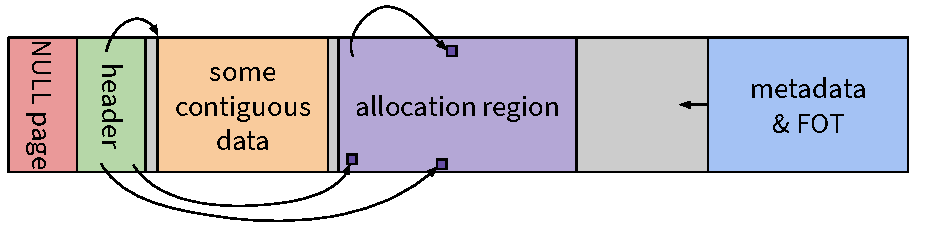
\includegraphics[width=\linewidth]{fig/typobj}
    \caption[Typical object layout]{A typical object layout. The header, contiguous region, and allocation region are all
        optional, however most objects will have a header. This object contains a number of internal
        pointers between regions. The metadata region (which includes the FOT) grows downward.}
    \label{fig:typobj}
\end{SCfigure}

Figure~\ref{fig:typobj} shows a typical object in Twizzler. The NULL page is always present to trap
NULL pointers, and is followed by a header. The application setting up this object may have a region
of some contiguous data (such as some strings, or an array), and may point to it from the header.
The object may have a region setup for allocation so that a future application using this
object can easily allocate and free memory when manipulating the object. Finally, the FOT and
metadata regions start at the top of the object and grow downwards.

\paragraph{Ensuring Base Type Properties}

When accessing persistent or shared data for the first time, it's necessary to specify the type of the data. For
objects, this means we need to specify the type of the header, as objects are typed by their header (also called the
object ``base''). While in C the function that gives access to the base returns a \texttt{void *}, the function in Rust
returns a reference to the specified base type. From there, any other data accessed traverses data structures that use
the type system. Twizzler invariant pointers implementation in Rust are typed, and the mutability rules ensure that our
transaction engine properly ensures transactional properties, then any data to which we can get a reference is
well-typed as long as the header of the object is well-typed.

To ensure this, we encode, in the object's metadata, a pair of 64~bit numbers that refer to a unique ID of the header
type\sidenote{This is currently allocated manually, though we plan to automatically generate the IDs via procedural
    macros in the future.} and a version number. When code tries to access the header, we do a one-time check to see if the
recorded ID and version match the ID and version from the type that we are supposed to return. If they fail to match, we
can return an error, and if they do match, then we know it's the correct type (up to collisions in the ID space, that is).

\section{The Flipside}

One aspect of programming for \NVM that is somewhat orthogonal to Twizzler's primary object model is considering what
effects writes will have to the actual physical media. This kind of consideration is common---we think about block
layouts and overwrites when considering differences between magnetic disk and SSDs---but for \NVM, we should ask what
the new device characteristics are, since
it is important that systems are optimized to leverage their
strengths and avoid stressing their weaknesses. We typically try to reduce writes to physical media, however with
\NVM it turns out that the number of \emph{bits flipped} may be the more important metric.

\NVMs such as PCM suffer from both wear and energy use when it must flip a stored bit. Applications such as IoT devices
cannot tolerate wear out and energy use as easily as other applications, and these devices make good targets for the
already dense and power efficient \NVM technologies.
Flipping a bit in PCM cells consumes $15.7\mathit{-}22.5\times$ more power than reading a
bit~\cite{dhiman_pdram:_2009,lee_architecting_2009,xiangyu_dong_nvsim:_2012,qureshi_scalable_2009}, and causes wear
(whereas reading does not cause nearly as much wear).
Thus, controllers can optimize by examining bits to determine which must actually change on a write~\cite{yang:iscas07}.
Of course, such an optimization is heavily dependent on software, which issues the writes.
Reducing bit flips, an optimization goal that has yet to be
sufficiently explored, can thus both save energy and extend the life of \NVM, but we optimize better if we manage to
design software to reduce bit flips.

We examined a number of different common data structures and examined strategies for how we can reduce bitflips caused
by data structure updates. This involved taking previously-known tricks like XOR linked lists~\cite{xorll} and
generalizing them to trees and hash tables, along with choices for bit packing and data layout, and modifying Gem5, a
system simulator, to count bit flips. We found that we could easily reduce a significant number of bits flipped in the
data structures we studied with little performance impact. Since the details are not germane to the Twizzler programming
model, details of our work on bitflipping are included in Appendix~\ref{app:bitflip}.


\section{Crash Consistency}
\label{sec:crash}

\Twizzler provides primitives for building crash-consistent data structures. At a low level,
it provides mechanisms for writing back cache-lines, appropriate fences, and basic transactions.
Applications use these primitives today outside of \Twizzler to build up larger, more complex support for
crash-consistent data structures.
%, thus we provide similar primitives.


\paragraph{Persistent Memory}

Programming against persistent memory has some advantages compared to programming against volatile memory and needing to
flush dirty pages to stable storage. Not only is it much faster, but failure-atomicity of an \NVM data structure can be
maintained by the application alone (if it so desires).
Our goal is to provide low level primitives without restricting programs or prematurely
prescribing particular solutions. There is a wealth of research on crash-consistent
data structures for
\NVM~\cite{condit:sosp09,coburn:asplos11,volos:asplos11,dulloor:eurosys14,narayanan:asplos12,ni:hotstorage18,ni:micro19,ogleari:hpca18,lu2014loose},
but it is still in flux. Of course, \Twizzler manages \emph{system} data structures,
such as FOT entries, views, \emph{etc.}, in a
crash-consistent manner using the aforementioned primitives, locking, and fencing.

\begin{SCfigure}
    \centering
    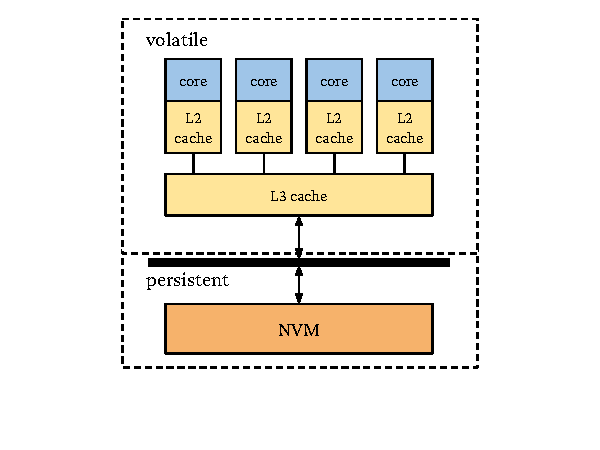
\includegraphics[width=\linewidth]{fig/vpdomains.pdf}
    \caption[Volatile and persistent domains]{Volatile and persistent domains. Once the memory controller has acknowledged the write, the system guarantees persistence of the write.}
    \label{fig:vpdomains}
\end{SCfigure}



At the time of writing, Intel systems handle \NVM by enabling a certain level of control over the cache system by
applications, notably via the \texttt{clwb} and fence instructions. Figure~\ref{fig:vpdomains} shows the boundary
between persistent and volatile domains in an abstracted CPU that operates roughly like how Intel's do. In this model,
any data stored in the cache is volatile, and will be lost if power is lost. Any data that makes it to the memory
controller (for which the memory controller acknowledges the write) is persisted. A small amount of internal residual
power is used by the persistent memory device to ensure the writes that reached the memory controller are stable.

With this model in mind, we can ensure failure atomicity in a rather inelegant manner if we use the \texttt{clwb}
instruction to ensure cache lines are flushed and the appropriate fence instructions to ensure durability, and end up
with a programming model reminiscent of multithreaded code using fences. We can abstract this a little bit to allow the
flushing of \emph{types} so as to avoid the programmer having to think entirely in cache lines. However, this still is a
lower level than most programmers likely want for ensuring safety. While Twizzler does provide a set of interfaces for
persisting data at this level, it also supports a basic transactional interface.


\paragraph{C Transactions Interface}
\Twizzler provides a transactional-persistent logging mechanism.
Programmers can write \texttt{TXSTART}--\texttt{TXEND} blocks to denote transactions and \texttt{TXRECORD}
statements to record pre-changed values. This is similar to the mechanism provided by
PMDK~\cite{libpmem}. If applications need more complex
transactions using different logging mechanisms, they can use libraries. \Twizzler's internal data
structures and \libcore's manipulation of object metadata is handled via a combination of these
transactions and cache-line writebacks.


\paragraph{Rust Transaction Interface}

The Rust interface to transactions is much safer than the C version, as it actually enforces various rules about type
safety, aliasing, and mutability. An example transaction block is written like,

\begin{lstlisting}[language=Rust]
    obj.tx(|tx| {
        let base = obj.base_mut(tx); // :&mut BaseType
        base.do_something();
    });
\end{lstlisting}

Here we start a transaction and get access to a transaction handle (\texttt{tx}). When we want to get a mutable
reference to part of the object, we must pass in a transaction handle, and the only way to get a transaction handle is
via the \texttt{tx} function. Thus we can enforce the aliasing rules for Rust inside the transaction framework.

\paragraph{Thread Restart}

\Twizzler provides a mechanism for restarting threads when power is restored following a crash.
Since views are persistent objects, all objects mapped during a thread's execution are known across
power cycles, and are mapped back in. The thread is then started at a special \texttt{\_resume}
entry point, allowing the program to handle the power failure in an application-specific manner.  Of
course, \emph{volatile} objects will be lost when power resumes, and thus any attempted access to
these objects will result in an exception. Thus applications that wish to resume after power failure
will need to be aware of and handle this. We do not wish to prescribe any restrictions
here---applications that want to place their heap in volatile memory for performance or security
reasons should be allowed to. We expect higher level support for applications to manage persistent
data, such as language support for persistent heaps, to make use of the features we provide, so
applications that want to resume can put resuming information in persistent objects.

The reason we choose to restart threads at a known, different entry point from normal application
start up is that in current systems, there is always volatile computation state (\eg registers, the
cache) that is lost when power is lost. Of course, in the future, systems may be able to prevent the
loss of more and more ephemeral computation state (with the logical extreme being perfect
resumability). In this case, the \texttt{\_resume} handler can be a simple stub that resumes the
execution exactly as left off. The more likely case, periodic checkpointing, can be similarly
handled, with the \texttt{\_resume} handler selecting the most recent valid check point to resume
from. The \texttt{\_resume} handler enables all of these solutions, thus remaining applicable across
hardware evolution.
\section{Memory Safety and Lifetimes}

One final aspect of objects is safety, that is, ensuring proper typing of memory and ensuring that object memory does
not leave a dangling reference behind. Twizzler accomplishes the general ideas of memory safety via a combination of
some runtime checks, some kernel support for specifying lifetime relationships between objects, and some language
support.
%Notably, using the Rust bindings provides significantly more memory and type safety than the C bindings do.

\subsection{Object Types, Persistence, and Lifetime}

%% TODO ensure these types are consistent with previous chapter.
Applications need to be able to specify what \emph{type} of memory an object resides in. Currently,
we are operating on systems that contain both persistent \NVM and volatile DRAM as main memory, and
applications may want to make use of both of these memory types. Placing certain objects in DRAM,
for example, can result in performance improvements (\eg caching read-only objects) or security
improvements (\eg making temporary key material volatile). \Twizzler exposes this choice to
applications at object creation time, allowing them to specify the type of the object. At least two
types, \emph{volatile} and \emph{persistent}, are supported by default. As additional types of physical memory
are added to systems (\eg different kinds of \NVM with different properties, high-bandwidth memory,
\etc), applications may wish to have more fine-grained control over where objects are placed, and
\Twizzler's APIs allow such control. Objects can also be moved between types of memory after
creation, though this may be a time consuming operation as it involves copying potentially large
amounts of data.

By default, objects are persistent and live in kernel-managed \NVM unless they are marked as
volatile. If an object is volatile, it has a limited lifetime that is related to the power state of
the machine---as soon as power is lost (or the system is rebooted) all volatile objects disappear.
Note that \Twizzler removes the distinction between volatile and persistent objects for how
applications \emph{access} data, relying on higher-level language or library support and application
support for dealing with the limited lifetime of volatile objects.

The property of persistent versus volatile for objects differs from the concept of
ephemeral data. The ``volatile'' property places a physical restriction on the lifetime of an object (the machine's
power state), while the ``persistent'' property indicates that the object will exist until
explicitly deleted. Objects can also be long-lived or ephemeral independent of their persistence
property, since we use the term ``ephemeral'' to describe information, data, or state that has a
finite lifetime and is expected to ``go away''. While all volatile objects are ephemeral, the
reverse is not true---we may place ephemeral data in a persistent object to allowed for recovery
after an unexpected power cycle. The ``persistent'' property of an object is a recorded piece
of information that the kernel associates with an object, but there is no such information for ephemeral
versus long-lived. Instead, we provide a mechanism for specifying a logical lifetime of objects
relative to one another with a mechanism called \emph{ties}, which we will discuss below.

\subsection{Object Ties and Logical Lifetime}

\iffalse
    Objects are, by default, persistent and live in kernel-managed \NVM. During creation, an object may
    be marked as ``volatile'', allowing the kernel to allocate memory for it from DRAM. This is useful
    for temporary application data that does not need to be persistent, such as stacks or volatile
    heaps. At any time, an object may be changed from volatile to persistent, or vice versa, but this
    may be a time consuming operation. Note that, although \Twizzler does distinguish between volatile
    and persistent objects (and allows applications to choose based on some policy what their objects
    are), \Twizzler removes the distinction between them when it comes to accessing the data.

    Throughout the paper, we use both terms ``volatile'' and ``ephemeral'' for different purposes.
    Volatile is a property of hardware---the data goes away when power is lost. We expose this meaning
    in objects that are marked as ``volatile'' to allow application to capitalize on the benefits of
    volatile memory (both performance and security). Ephemeral, more broadly, describes information,
    data, or state that has a finite lifetime and may ``go away''. This is in contrast to persistent
    data which has an ``infinite'' lifetime, and volatile data which has a finite lifetime tied to the
    power state of the machine. All volatile objects are ephemeral, while the reverse is not necessarily
    true (\eg an application may have some temporary state that it makes persistent to recover from a
    power cycle).
\fi

%An example of ephemeral data is temporary application data like a stack or a heap.
Applications in \Twizzler also have some lifetime; an application's job is typically to operate on
some persistent data while performing some computation before eventually exiting. Such an
application will likely use volatile objects to represent temporary computation state (\eg the
stack and heap, which are ephemeral). However, just assigning an object as volatile is insufficient
because there is a lifetime mismatch: the volatile object will live until the next reboot while the
application may exit before then or may even live and try to recover after a power cycle.
Manually deleting the volatile object when the application is done is also insufficient, as it does
not account for crashes where the application may be unable to clean up its state. Furthermore,
applications that wish to support recovery may make use of persistent stacks and heaps, thus these
objects would have to be persistent despite being ephemeral.

While we could provide a mechanism designed specifically for this ``system-level'' task,
where the kernel maintains a set of objects to automatically cleanup when an application exits, this
would require the kernel to have some understanding of what an ``application'' is. Furthermore, if
we generalize a solution to automatic cleanup, we can allow applications to make use of it for their
own purposes. For example, in \unix, it is common for programs to create and immediately unlink
files to ensure the system frees those resources when the program exits. We would like to reproduce
similar semantics here that also solves the lower level problem above of freeing application state
by assigning a lifetime to objects that is more expressive than simply ``volatile'' and
``persistent''.

\iffalse
    Applications need a mechanism to express the relative lifetime of objects in the system to ensure
    that a given object exists at least as long as another object. Specifying object lifetimes is
    commonly used to enable automatic cleanup. For example, in \unix, programs often create and
    immediately unlink files to ensure the system deletes them on exit. Similarly, a lot of ephemeral
    resources that applications typically use (\eg the stack, the heap) are formalized as objects in
    \Twizzler\sidenote{Formalizing these resources as objects both simplifies the programming
        environment model and allows them to be optionally persisted, allowing applications to resume their
        state after crashes.}.
\fi

In \Twizzler, object lifetime is expressed through \emph{ties}.
An object can be tied to another by invoking a system call that tells the kernel that
object \texttt{A} is tied to object \texttt{B}, after which the lifetime of \texttt{A} is
guaranteed to be at least that of \texttt{B}. The kernel will not fully delete object \texttt{A} (even if the
delete system call is invoked on it) until after \texttt{B} is fully deleted. An object may be tied
to a large (but finite) number of other objects and may also be \emph{untied} at any time. This
model of specifying object lifetime relative to others is similar to Rust~\cite{rust}, where
reference lifetime can be named so that the programmer can express lifetimes of objects relative to
each other. Note that object ties are not related to invariant pointers (discussed in more detail
in Chapter~\ref{ch:invariant}), and instead primarily provide a way to formalize automatic cleanup.


Object ties provide a convenient mechanism for applications to build large data structures across
multiple objects without giving up easy cleanup if something goes wrong or if the ``root'' object is
deleted. \Twizzler also uses ties internally: when an object is created as copy-from an existing
object, it uses copy-on-write semantics, and thus internally marks the source object as tied to the
new object. We also tie ephemeral program state objects to threads (which are also represented by
objects) such that they are automatically cleaned up when a program exits. It is our expectation
that application programmers will only rarely directly use ties. Instead, we expect that ties will
provide necessary features that higher-level programming language support for persistent memory can
use.

Note that object ties interact with the notion of volatile and persistent objects, because
volatile objects have an implicit \emph{maximum} lifetime---that of the next machine restart or
power loss. Tying volatile objects to volatile objects and persistent objects to persistent objects both act as
expected. Tying a persistent object to a volatile object is also semantically simple (persistent
objects already have an ``assumed lifetime'' that is longer than a volatile object). Tying a
volatile object to a persistent object, however, may seem somewhat nonsensical. However, \Twizzler
does still allow this because it has useful semantics: if an application creates a data structure
with some volatile component\sidenote{Since \Twizzler's kernel is not involved in reference
    creation, it cannot prevent such a reference from being created. We expect language support for
    persistent data structures to impose restrictions on applications in this regard, and the OS should
    not prematurely restrict how applications use volatile and persistent objects. Access to a volatile
    object that no longer exists after a reboot results in a simple access fault, mitigating security
    concerns.},
%\footnote{We will discuss the implications of creating references
%between volatile and persistent objects in \S~\ref{twz:pptr}.}
it may want to tie the lifetime of that volatile component to the
persistent component if the data structure is to be deleted. This use case (creating a persistent
object that we expect to delete) is not uncommon, particularly in applications designed to recover
partial computation after a crash. Note that, in this case, the maximum
lifetime of the volatile object is still in-play; after a power cycle, that object will no longer be
present, so tying a volatile object to a persistent object is somewhat dangerous.


\subsection{Safe Allocation}

As we discussed above, an object may optionally have a region within which we rely on an object memory allocator to
organize memory. However, when objects may persist or be shared, there are some additional hazards to consider.

\begin{enumerate}
    \item \textbf{Crash Consistent}: The allocator must allow for power interruptions or application failures, and so
          all operations must be failure-atomic.
    \item \textbf{Leaked Memory}: Say we allocate some memory from an object, and let's consider the interface described
          by \texttt{malloc} and \texttt{free}. We can imagine a situation where an application allocates some memory, but
          before we manage to store the pointer anywhere, the power is reset. Or, alternatively, after a node is removed from,
          say, a list, but before the call to \texttt{free} is made, the power dies. In both cases the memory is leaked, and
          cannot be recovered without some application-specific \texttt{fsck}-like check.
    \item \textbf{Dangling Pointers}: Imagine that same scenario with freeing a node, but this time, the order of operations
          (remove node, then free) is not specified\sidenote{This could happen to improper use of transactions or persist
              barriers.}. Or, similarly, we allocate some memory and write a new node, and link it, but the order of operations is
          wrong again. Both of these cases result in writing a pointer to memory considered freed by the allocator.
\end{enumerate}

One might wonder if there concerns are specific to \NVM, where hardware persists behind a curtain, or more generally,
perhaps when we are flushing periodically to disk. Certainly we must worry about the above issues if hardware is
controlling persistence, but we still care even without \NVM. The \emph{semantics} of accessing an object are of sharing
it or not (recall from Chapter~\ref{ch:datacentric} that persistence \emph{is} sharing), and thus once it's shared it
could be in multiple places in space and/or time. We must, therefore, make allocation and resource acquisition, and
deallocation and reference removal failure-atomic. Consider a case where we interrupt an allocator operation after part
of the allocator state is persisted to disk and the power fails. The problems above still exist, even for persistent
objects stored on a disk or SSD.

To properly have an allocator that works on shared objects, we must build it to be \emph{internally} crash consistent and
present an external interface that allows applications to ensure \emph{external} crash consistency.
To do this, we will
need to\sidenote{Thankfully!} change the interfaces to something richer than \texttt{malloc} and \texttt{free}:

\begin{lstlisting}[language=C]
    int alloc(object *obj, size_t len,
        void **owner, uin64_t flags,
        void (*ctor)(void *mem, void *data), void *data);
    int free(object *obj, void *p,
        void **owner, uint64_t flags);
\end{lstlisting}

The allocate function is built around an allocation and construction pattern that follows three steps:
\begin{enumerate}
    \item Allocate memory from the allocator.
    \item Construct the memory into a valid inhabitant of the intended type.
    \item Record the reference to the node into some data structure.
\end{enumerate}

And that the freeing pattern occurs in two steps:

\begin{enumerate}
    \item Remove the final (or only) pointer to the to-free memory by overwriting it (or clearing it to NULL).
    \item Free the memory back to the allocator.
\end{enumerate}

These steps are vital for persistence-safety, and it is vital that they occur in that order. Permuting the steps can
allow for any of the problems we discussed above, and these steps are all needed to properly allocate an instance of
a type and record a reference to it.

Internally, the allocator keeps an undo log for the operations performed by the allocator functions. When allocating, a
region is selected and removed from internal data structures. The operations to remove the memory region from internal
data structures are recorded to the log. The constructor function (the \texttt{ctor} argument) is called on the memory region. After the constructor
function completes, the region is flushed to memory for persistence safety. Next, data pointed to by the \texttt{owner}
argument pointer is recorded into the log, thus ensuring we cannot have dangling pointers. Finally, the value at
\texttt{*owner} is written with the new invariant pointer to the allocated region, and the log is flushed.

The above allocation algorithm is safe because it ensures that, if the log is replayed, all internal data structures will
be reset to contain the region, and the owner pointer is also reset to prevent the (now unallocated) region from being
referenced. Since the region was not allocated, we can assume that none of that memory is referenced externally, and the
contents do not matter\sidenote{For example, we can use that region for allocator-internal data structures!}. Thus we
can assume that region was filled with uninitialized memory, and we do not need to restore it\sidenote{Any data
    structure internal data that needs to be restored inside the region will be properly reset by replaying the log.}. This
is not a mere optimization for restoring after a crash, nor is it an optimization for bulk flushes during allocations,
it is vital for efficient implementation. The total amount of memory that needs to be flushed is $O(s)$, where $s$ is
the size being allocated, because we have to flush the entire memory region that holds the type for which we are
allocating and the size choice is controlled by the caller. However, the number of items we record to the log is
controlled by the allocator implementation, and can be made $O(1)$.

For any internal operation, we count the number of items it has to add to the log, \eg, if we remove a region from the
free list, split it, and add one part to the free list, how many log records are created by those list operations.
Since those are fixed operations, we can count the total number statically. If, however, an allocator custodial function
run an unspecified number of times, we cannot be sure ahead of time how many operations it will perform (\eg, merging
nodes in a list depends on the number of mergeable pairs, which depends on the length of the list). For these
operations, we define a maximum allowed number of log entries, and break out of loops early if we run out. Thus we only
need to count the number of operations \emph{per iteration}, and then tweak the maximum log entries to allow most such
loops to run for several, but a bounded number of, loops. As a result, we can set a maximum log length and allocate it
statically within the region, instead of having to handle a variable and unbounded number of entries due to either
internal or external causes.

\iffalse
    \section{Patterns, New and Old}

    It's worth taking a look at some patterns and expected software uses of the Twizzler model. In particular, the newly
    enabled optimizations and patterns that emerge from a global address space and a lower level understanding of data relationships.

    \subsection{Progressive and Immutable}

    Of particular interest for optimizations are the class of \emph{progressive} objects.
    We call an object $O$ progressive if,
    given any two derived versions $O_1$ and $O_2$ of $O$, there is a unique object $O_m$ that incorporates all of the changes in $O_1$ and $O_2$.
    Immutable objects are trivially progressive, since they do not change.
    In the distributed systems literature, Conflict-free Replicated Datatypes
    (CRDTs)~\cite{shapiro2011comprehensive}
    are an important class of progressive objects.

    A system with explicit, context-free identity can unlock the power of progressive objects.
    These objects may always be replicated, and aggressively pushed towards
    sites where they are likely to be used.
    Anywhere along the way, divergent copies of progressive objects may be eagerly and automatically
    merged---even when the end-point applications that use the objects are nowhere to be found.

    % TODO: make sure this is talked about earlier
    Of course, the ``merge'' operation to compute $O_m$ may not be known to the OS; however, our
    ability to rendezvous both code and data throughout the system allows us to manifest the required
    applications where desired. Data objects themselves can identify what ``kind'' of object they are or
    what code objects are necessary to complete a merge.
    Thus if a particular node receives two divergent copies of a particular object, it can consult the
    object's metadata to determine what code to run to merge the two before forwarding the final object,
    $O_m$, all without consulting the end-point applications or performing some complex global
    coordination.

    %\todo[inline]{
    %Talk about how we can move around small pieces of "merge" code that can merge objects. Talk about
    %how objects can encode identifiers that describe what APIs they "respond" to.}

    \paragraph{Improving Prefetching}
    \label{sec:prefetch}

    Prefetching leverages spatial locality to improve future performance. A typical example is
    reading adjacent disk sectors under the assumption that their adjacency indicates that they
    will soon be needed. This example illustrates a common use of some proxy in place of actual data
    identity---this only works because file systems often try to lay out data in this way, and
    applications are optimized to take advantage of that layout. This, however, is \emph{extremely}
    fragile; the data may be unrelated, and the system cannot know this. Over a network, prefetching is
    often implemented in application specific ways, \eg, HTTP pushing additional resources that have
    not yet been requested. However, these relationships are, in general, undiscoverable by the system,
    limiting other applications to be beholden to each other in brittle ways
    and removing the benefits we could have with a more general automatic data movement
    model.

    When object relationships are explicit and can be interpreted to some extent by the
    system without help from applications, we can imagine an ``object graph'' that represents the
    relationships between objects. An example is shown in Figure~\ref{fig:ograph}, where
    an application has some ``root'' data object that refers to an index for a database, which in turn
    has references to data within some data object. Both the index and the data object (say they are
    CRDTs) provide the system with a reference to some merge code.

    Twizzler's FOT instantiates this object graph; it is understood by \emph{any} application
    and thus \emph{the system itself}.
    Of course, the system cannot have a
    perfect understanding of all the details of a data relationship---a particular external reference
    may be rarely used, or only used in a specific circumstance---but at least a translucent view of
    what objects may be accessed from a particular object can be useful to the system as a whole.

    \begin{SCfigure}[t]
        \centering
        \includegraphics[width=\linewidth]{genfig/obj_graph.pdf}
        \caption[Example object graph]{Example object graph.}
        \label{fig:ograph}
    \end{SCfigure}

    An immediate consequence is that prefetching can be done based not on some proxy for identity,
    but instead on that identity itself. The system may not know for certain that object $A$ will
    reference object $B$, but it does know that it might, and will \emph{not} reference other objects.
    Because we have an end-to-end notion of identity, we can do this prefetching in the network itself,
    largely without application support.
    This dovetails nicely with progressive objects, as they enable aggressive pushing of objects around
    the system. Since object merging can be done \emph{anywhere}, it makes sense to prefetch objects
    more aggressively than in a system where this cannot be done.


    \subsection{Conventions Not Constraints}

    One might think we are suggesting all applications be written in a constrained data
    model, but this is not the case! While such a model has benefits as discussed above, it is
    important that our system design does not curtail applications' freedoms in how they design their
    data models. Many patterns in distributed systems require high-conflict objects (\eg mutexes), and
    while our system should provide benefits where possible it should not prevent these concepts from
    being represented.

    In particular, we support existing solutions and models. Traditional consistency and
    consensus algorithms that rely on machine identity to organize fault-tolerance zones still work (see
    Section~\ref{sec:name_machines}). Support for data with changing identity at run-time or data whose
    identity is not statically known can use late-binding, which our model explicitly makes
    allowances for (see Section~\ref{sec:latebinding}). Support for standard message-passing and RPC
    applications is encouraged by our model, as providing APIs to protect data access is a vital part of
    building complex systems; our end-to-end notion of identity facilitates this through the ability to
    refer to data without additional coordination. Objects with arbitrarily changing contents can be
    implemented through these methods, allowing applications like lock servers or complex databases to
    operate as usual.

    %While we get a significant benefit in a somewhat more constrained data model as discussed above, we realize that
    %not all systems and data fit that model. Thus it is important that we design our system in such a
    %way that we do not limit the generality and flexibility of applications that want to perform
    %arbitrary updates to data.

    %Of course there are challenges beyond those presented here; consistency and consensus, to name two examples,
    %are well studied and are we make no attempt to suggest that they should be ignored or replaced.
    %Indeed, our model makes room for allowing more complex applications to use these tools whenever
    %necessary.

    \subsubsection{Late-binding of Names}
    \label{sec:latebinding}

    A disadvantage of context-free references is the lack of late-binding of names,
    since late-binding occurs at the time that a reference is followed. This feature
    is vital, as it enables the construction of references to data that changes
    over-time (\eg shared libraries). While support for late-binding
    introduces \emph{some} context back into references, it does so in a controlled way. In Twizzler,
    instead of storing a GUID in an FOT entry, we can store a string and a reference
    to a name resolution function.
    This means
    that while a particular reference uses late-binding, the system can still compute the binding itself
    if necessary.

    Data relationships often do not require this.
    A common pattern is to construct some object graph (like
    Figure~\ref{fig:ograph}) and then name a single object as an ``entry point''.
    Names and late-binding in Twizzler are an overlay to data's actual
    identity, resulting in a ``two-level'' naming system that can use human-readable names to facilitate
    discovery for a more authoritative name (the GUID).
    %If a relationship between two object is ``tight'', then it would make sense to encode this
    %without late-binding. However, if a 


    %\todo[inline]{
    %Global name service ... }


    \subsubsection{Explicitly Naming Machines}
    \label{sec:name_machines}

    In our model, we usually refer to data without mixing machine identity into references,
    largely removing the need to identify machines themselves.
    However, at least for locality reasons,
    an application should be \emph{able} to identify and access a resource on a
    specific machine as part of its API---a particular
    %either run computation there or access data located on a \emph{specific} machine---a particular
    machine may control some physical device or resource or be an interface to some other system. This
    has been explored before~\cite{ousterhout:computer88,grapevine}; we explicitly allow for this
    throughout our system.

    Our model does not \emph{prevent} applications from adding notions of locality and
    machine identity to its API; instead, our goal is to move away from this as the \emph{default}
    construction.
    Twizzler has the ability to create ``control'' objects whose identities can be used
    where machine IDs or process IDs would normally be. This allows applications to talk about ephemeral
    actors with the same ``language'' as that of permanent data, which combines well with the
    late-binding mechanism discussed above. For example, applications could create references to ``the
    current coordinator node'' whose identity changes over-time.

    \subsubsection{Sharing in Heterogeneous Environments}

    Extending data structures through a heterogeneous environment is itself a challenge, as different
    machines interpret data in different ways. This is actually not a problem unique to distributed
    environments, however, as we see this cropping up in single-node systems as well. Of course, the
    ``explicit encoding of references as pointers'' model does \emph{not} require that all data be
    expressed as C structs. In fact, it is \emph{rarely} the case that complex distributed applications
    need or should have such a low-level view of data. Instead, higher-level languages that can already
    encode data in formats that allow for heterogeneous interpretation can also leverage explicit
    references as we have defined in our model.


    \subsubsection{Decoupling Through Coupling.}
    %
    There is an irony in our vision for decoupling applications in a more
    flexible manner than RPC: this vision requires a \emph{stronger}
    coupling between the OS and the network.
    Pushing data identity into the OS and the network as a first-class
    abstraction has a number of benefits, but it does imply more rigidity
    in the lower-level infrastructure. We argue that this is okay, and even desirable. Our
    goal is to provide \emph{applications} with flexibility, scalability,
    and generality. By moving some application-level semantics
    like data references and identity into the lower-level system, we
    can implement in one place patterns like caching, prefetching, and
    query planning that often get reimplemented at many layers
    %(including
    %the application)
    \emph{because} these layers lack a common language to
    talk about data.
    %Our plan is to explore the trade-offs between lower level rigidity and application
    %flexibility.


    \subsubsection{Uniformity Between Code and Data.}
    %
    Recently, Wang et al.~\cite{wang:hotos21} proposed an extension to RPC
    that passes first class immutable references as well
    as values in procedure calls and returns.  The goal is to preserve the
    functional semantics of RPC while permitting the underlying system to
    avoid unnecessary copies and to perform memory management.  Their
    design is a step in the right direction, addressing some of the
    weaknesses of RPC, by making it possible for the system
    to transparently move data.  But, it only takes us halfway: RPC remains
    compute-centric and programmers must indicate
    \emph{where} code should execute.
    %For example, the optimization
    %described in Section~\ref{sec:example} in which Dave (the powerful
    %edge device) performs inference locally could not be realized via
    %\emph{any} RPC mechanism. 
    In our system, code (like data) is global
    and referenceable from anywhere---there would be no reason to provide a
    separate mechanism for specifying function invocations. Instead, we
    place all data \emph{and} code in a single space, allowing code
    and data to reference each other. This dramatically improves
    expressivity, decoupling, and reuse, as we can now rely on the system
    to move not only data but also code to where it needs to be on demand
    without manual intervention and setup. In our model, the programmer
    primarily \emph{orchestrates a rendezvous between code and data}.


    \subsection{The Hard Stuff}

    Running computations on a collection of loosely-coupled machines that fail independently raises the specter of
    \emph{partial failure}.  Machines may fail by crashing or becoming unreachable, conditions which
    can be difficult to detect. Care must be taken such that applications produce correct and complete
    results when partial failure is possible.  There have been decades of scholarship on
    fault tolerance~\cite{gray-dbos,3pc,bully,whydo,primary-site, primary-copy, thomas-quorum,paxos,zab}
    and we prefer to keep our design compatible with existing or emerging mechanisms rather than providing a single solution.
    We believe that the features of Twizzler---in particular, invariant, context-free data references---will simplify the implementations
    of existing fault-tolerance and durability mechanisms because they remove the need to update data
    when locations change and allows machines to participate in these algorithms with less
    application-specific global coordination.

    Many fault tolerance mechanisms employ \emph{replication} to guard against data loss that may occur
    due to component failure.
    Unfortunately, replicating data gives rise to \emph{consistency} concerns: ensuring that replicas agree on their state,
    or at least ensuring that they can eventually converge to a common state.  Like fault-tolerance, consistency of replicated data
    is a nuanced area.  We believe it would be a mistake to select a one-size-fits-all solution.  Instead our aim is to support
    %(and in
    %some cases facilitate)
    state-of-the-art and emerging solutions.
    \iffalse
        \unedit{
            \paragraph*{Limitations and Challenges.}
            %
            Many challenges lie ahead. Perhaps foremost among them is the tension between partial failure
            (inevitable in any distributed system), fault tolerance, and mechanisms that attempt to hide the
            movement of computation and data~\cite{waldo}.  Masking failures via replication gives rise to
            concerns about consistency; mechanisms that ensure consistency in the presence of possible conflicts
            are costly in general.  We plan to address these challenges along two separate axes. At the level of
            the system co-design, we will experiment with offloading some synchronization and
            arbitration~\cite{jin18,jepsen18} concerns to the programmable network (which now
            functions somewhat as a memory bus), letting us explore the consistency and coherence space
            together.  At the level of programming model, we will explore how a whole-system view of object
            identity and references can interface with languages to support patterns for weakly
            consistent replication, such as auto-merging progressive objects like
            CRDTs~\cite{shapiro2011comprehensive} during data movement.
        }
    \fi

\fi



\begin{chconc}
    Ensuring that programmers have access to a reasonable programming model that sits atop the operating system
    abstractions built for it is of utmost importance. Even if the lower levels of the systems provide access to a fast,
    invariant reference in a global address space that simplifies data models and transformations, programmers still
    need systems that make some of the harder parts easier. Twizzler provides a set of higher level APIs that enable
    day-to-day tasks like allocations and ensuring crash consistency are consistently handled by the system.
\end{chconc}




\chapter[Concrete Concerns and Other Opportunities]{Concrete Concerns and \linebreak Other Opportunities}\label{ch:concrete}

\section{Persistence}

\subsection{Failure-Atomicity}

\begin{SCfigure}
    \centering
    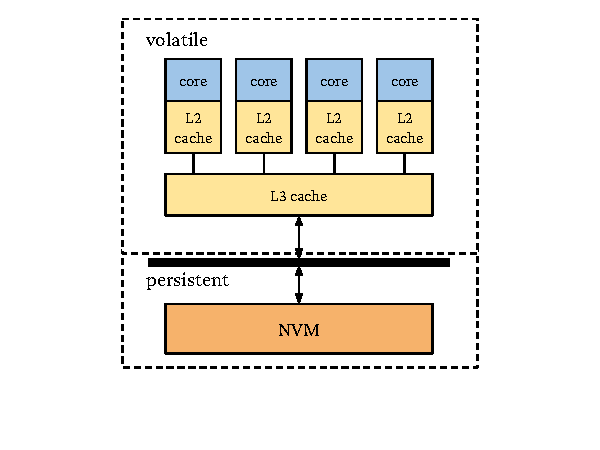
\includegraphics[width=\linewidth]{fig/vpdomains.pdf}
    \caption{Volatile and persistent domains on Intel CPUs. Once the memory controller has acknowledged the write, the system guarantees persistence of the write.}
    \label{fig:vpdomains}
\end{SCfigure}
\subsection{Bit Flipping}

\section{Distribution}

\unedit{
    Two fundamental changes arise as we distribute our data-centric system model---changes that present unavoidable challenges
    as well as new opportunities.  Given a multiplicity of loosely-coupled computers with independent storage and computing capabilities,
    we now need to consider both how data is \emph{shared} among computers, and how to schedule the \emph{rendezvous} between data
    and programs necessary to effect computation.

    It turns out that the key feature of Twizzler---explicit, context-free data identity---allows us to
    completely rethink system support for sharing and rendezvous because data and node identity are
    decoupled.
    It becomes easier to distribute applications, as they need not worry
    about coordinating a ``view'' of the object space across systems, nor do they need to worry about
    data movement when constructing data and relationships. We can more easily embed program
    logic in network, leveraging ``smarter'' network hardware because it can
    operate on data (in a limited way) without help from end-point applications. Computation can be
    created (or defined) on one machine and run transparently on another---a boon for edge-type
    systems---or can be paused and resumed elsewhere
    without synchronizing shared identity context, or even cooperatively partially executed
    by multiple machines.
}

\subsection{The Good Stuff}


\unedit{
    \subsubsection{Progressive and Immutable}

    %When objects do not change, or change in predictable ways, explicit identity enables powerful optimizations.
    %In this section, we expand on what it means for objects to change predictably.  We then provide examples of....

    %\subsection{Progressive and Immutable Objects}

    Of particular interest for optimizations are the class of \emph{progressive} objects.
    We call an object $O$ progressive if,
    given any two derived versions $O_1$ and $O_2$ of $O$, there is a unique object $O_m$ that incorporates all of the changes in $O_1$ and $O_2$.
    Immutable objects are trivially progressive, since they do not change.
    In the distributed systems literature, Conflict-free Replicated Datatypes
    (CRDTs)~\cite{shapiro2011comprehensive}
    are an important class of progressive objects.

    A system with explicit, context-free identity can unlock the power of progressive objects.
    These objects may always be replicated, and aggressively pushed towards
    sites where they are likely to be used.
    Anywhere along the way, divergent copies of progressive objects may be eagerly and automatically
    merged---even when the end-point applications that use the objects are nowhere to be found.

    % TODO: make sure this is talked about earlier
    Of course, the ``merge'' operation to compute $O_m$ may not be known to the OS; however, our
    ability to rendezvous both code and data throughout the system allows us to manifest the required
    applications where desired. Data objects themselves can identify what ``kind'' of object they are or
    what code objects are necessary to complete a merge.
    Thus if a particular node receives two divergent copies of a particular object, it can consult the
    object's metadata to determine what code to run to merge the two before forwarding the final object,
    $O_m$, all without consulting the end-point applications or performing some complex global
    coordination.

    %\todo[inline]{
    %Talk about how we can move around small pieces of "merge" code that can merge objects. Talk about
    %how objects can encode identifiers that describe what APIs they "respond" to.}

    \paragraph{Improving Prefetching}
    \label{sec:prefetch}

    Prefetching leverages spatial locality to improve future performance. A typical example is
    reading adjacent disk sectors under the assumption that their adjacency indicates that they
    will soon be needed. This example illustrates a common use of some proxy in place of actual data
    identity---this only works because file systems often try to lay out data in this way, and
    applications are optimized to take advantage of that layout. This, however, is \emph{extremely}
    fragile; the data may be unrelated, and the system cannot know this. Over a network, prefetching is
    often implemented in application specific ways, \eg, HTTP pushing additional resources that have
    not yet been requested. However, these relationships are, in general, undiscoverable by the system,
    limiting other applications to be beholden to each other in brittle ways
    and removing the benefits we could have with a more general automatic data movement
    model.

    When object relationships are explicit and can be interpreted to some extent by the
    system without help from applications, we can imagine an ``object graph'' that represents the
    relationships between objects. An example is shown in Figure~\ref{fig:ograph}, where
    an application has some ``root'' data object that refers to an index for a database, which in turn
    has references to data within some data object. Both the index and the data object (say they are
    CRDTs) provide the system with a reference to some merge code.

    Twizzler's FOT instantiates this object graph; it is understood by \emph{any} application
    and thus \emph{the system itself}.
    Of course, the system cannot have a
    perfect understanding of all the details of a data relationship---a particular external reference
    may be rarely used, or only used in a specific circumstance---but at least a translucent view of
    what objects may be accessed from a particular object can be useful to the system as a whole.

    \begin{SCfigure}[t]
        \centering
        \includegraphics[width=\linewidth]{genfig/obj_graph.pdf}
        \caption{Example object graph.}
        \label{fig:ograph}
    \end{SCfigure}

    An immediate consequence is that prefetching can be done based not on some proxy for identity,
    but instead on that identity itself. The system may not know for certain that object $A$ will
    reference object $B$, but it does know that it might, and will \emph{not} reference other objects.
    Because we have an end-to-end notion of identity, we can do this prefetching in the network itself,
    largely without application support.
    This dovetails nicely with progressive objects, as they enable aggressive pushing of objects around
    the system. Since object merging can be done \emph{anywhere}, it makes sense to prefetch objects
    more aggressively than in a system where this cannot be done.

}


\unedit{

    \subsection{Conventions Not Constraints}

    One might think we are suggesting all applications be written in a constrained data
    model, but this is not the case! While such a model has benefits as discussed above, it is
    important that our system design does not curtail applications' freedoms in how they design their
    data models. Many patterns in distributed systems require high-conflict objects (\eg mutexes), and
    while our system should provide benefits where possible it should not prevent these concepts from
    being represented.

    In particular, we support existing solutions and models. Traditional consistency and
    consensus algorithms that rely on machine identity to organize fault-tolerance zones still work (see
    Section~\ref{sec:name_machines}). Support for data with changing identity at run-time or data whose
    identity is not statically known can use late-binding, which our model explicitly makes
    allowances for (see Section~\ref{sec:latebinding}). Support for standard message-passing and RPC
    applications is encouraged by our model, as providing APIs to protect data access is a vital part of
    building complex systems; our end-to-end notion of identity facilitates this through the ability to
    refer to data without additional coordination. Objects with arbitrarily changing contents can be
    implemented through these methods, allowing applications like lock servers or complex databases to
    operate as usual.

    %While we get a significant benefit in a somewhat more constrained data model as discussed above, we realize that
    %not all systems and data fit that model. Thus it is important that we design our system in such a
    %way that we do not limit the generality and flexibility of applications that want to perform
    %arbitrary updates to data.

    %Of course there are challenges beyond those presented here; consistency and consensus, to name two examples,
    %are well studied and are we make no attempt to suggest that they should be ignored or replaced.
    %Indeed, our model makes room for allowing more complex applications to use these tools whenever
    %necessary.

    \subsubsection{Late-binding of Names}
    \label{sec:latebinding}

    A disadvantage of context-free references is the lack of late-binding of names,
    since late-binding occurs at the time that a reference is followed. This feature
    is vital, as it enables the construction of references to data that changes
    over-time (\eg shared libraries). While support for late-binding
    introduces \emph{some} context back into references, it does so in a controlled way. In Twizzler,
    instead of storing a GUID in an FOT entry, we can store a string and a reference
    to a name resolution function.
    This means
    that while a particular reference uses late-binding, the system can still compute the binding itself
    if necessary.

    Data relationships often do not require this.
    A common pattern is to construct some object graph (like
    Figure~\ref{fig:ograph}) and then name a single object as an ``entry point''.
    Names and late-binding in Twizzler are an overlay to data's actual
    identity, resulting in a ``two-level'' naming system that can use human-readable names to facilitate
    discovery for a more authoritative name (the GUID).
    %If a relationship between two object is ``tight'', then it would make sense to encode this
    %without late-binding. However, if a 


    %\todo[inline]{
    %Global name service ... }


    \subsubsection{Explicitly Naming Machines}
    \label{sec:name_machines}

    In our model, we usually refer to data without mixing machine identity into references,
    largely removing the need to identify machines themselves.
    However, at least for locality reasons,
    an application should be \emph{able} to identify and access a resource on a
    specific machine as part of its API---a particular
    %either run computation there or access data located on a \emph{specific} machine---a particular
    machine may control some physical device or resource or be an interface to some other system. This
    has been explored before~\cite{ousterhout:computer88,grapevine}; we explicitly allow for this
    throughout our system.

    Our model does not \emph{prevent} applications from adding notions of locality and
    machine identity to its API; instead, our goal is to move away from this as the \emph{default}
    construction.
    Twizzler has the ability to create ``control'' objects whose identities can be used
    where machine IDs or process IDs would normally be. This allows applications to talk about ephemeral
    actors with the same ``language'' as that of permanent data, which combines well with the
    late-binding mechanism discussed above. For example, applications could create references to ``the
    current coordinator node'' whose identity changes over-time.

    \subsubsection{Sharing in Heterogeneous Environments}

    Extending data structures through a heterogeneous environment is itself a challenge, as different
    machines interpret data in different ways. This is actually not a problem unique to distributed
    environments, however, as we see this cropping up in single-node systems as well. Of course, the
    ``explicit encoding of references as pointers'' model does \emph{not} require that all data be
    expressed as C structs. In fact, it is \emph{rarely} the case that complex distributed applications
    need or should have such a low-level view of data. Instead, higher-level languages that can already
    encode data in formats that allow for heterogeneous interpretation can also leverage explicit
    references as we have defined in our model.
}


\unedit{
    \subsubsection{more shit}
    \paragraph*{Decoupling Through Coupling.}
    %
    There is an irony in our vision for decoupling applications in a more
    flexible manner than RPC: this vision requires a \emph{stronger}
    coupling between the OS and the network.
    Pushing data identity into the OS and the network as a first-class
    abstraction has a number of benefits, but it does imply more rigidity
    in the lower-level infrastructure. We argue that this is okay, and even desirable. Our
    goal is to provide \emph{applications} with flexibility, scalability,
    and generality. By moving some application-level semantics
    like data references and identity into the lower-level system, we
    can implement in one place patterns like caching, prefetching, and
    query planning that often get reimplemented at many layers
    %(including
    %the application)
    \emph{because} these layers lack a common language to
    talk about data.
    %Our plan is to explore the trade-offs between lower level rigidity and application
    %flexibility.


    \paragraph*{Uniformity Between Code and Data.}
    %
    Recently, Wang et al.~\cite{wang:hotos21} proposed an extension to RPC
    that passes first class immutable references as well
    as values in procedure calls and returns.  The goal is to preserve the
    functional semantics of RPC while permitting the underlying system to
    avoid unnecessary copies and to perform memory management.  Their
    design is a step in the right direction, addressing some of the
    weaknesses of RPC, by making it possible for the system
    to transparently move data.  But, it only takes us halfway: RPC remains
    compute-centric and programmers must indicate
    \emph{where} code should execute.  For example, the optimization
    described in Section~\ref{sec:example} in which Dave (the powerful
    edge device) performs inference locally could not be realized via
    \emph{any} RPC mechanism.  In our system, code (like data) is global
    and referenceable from anywhere---there would be no reason to provide a
    separate mechanism for specifying function invocations. Instead, we
    place all data \emph{and} code in a single space, allowing code
    and data to reference each other. This dramatically improves
    expressivity, decoupling, and reuse, as we can now rely on the system
    to move not only data but also code to where it needs to be on demand
    without manual intervention and setup. In our model, the programmer
    primarily \emph{orchestrates a rendezvous between code and data}.


}
\subsection{The Hard Stuff}

\unedit{
    Running computations on a collection of loosely-coupled machines that fail independently raises the specter of
    \emph{partial failure}.  Machines may fail by crashing or becoming unreachable, conditions which
    can be difficult to detect. Care must be taken such that applications produce correct and complete
    results when partial failure is possible.  There have been decades of scholarship on
    fault tolerance~\cite{gray-dbos,3pc,bully,whydo,primary-site, primary-copy, thomas-quorum,paxos,zab}
    and we prefer to keep our design compatible with existing or emerging mechanisms rather than providing a single solution.
    We believe that the features of Twizzler---in particular, invariant, context-free data references---will simplify the implementations
    of existing fault-tolerance and durability mechanisms because they remove the need to update data
    when locations change and allows machines to participate in these algorithms with less
    application-specific global coordination.

    Many fault tolerance mechanisms employ \emph{replication} to guard against data loss that may occur
    due to component failure.
    Unfortunately, replicating data gives rise to \emph{consistency} concerns: ensuring that replicas agree on their state,
    or at least ensuring that they can eventually converge to a common state.  Like fault-tolerance, consistency of replicated data
    is a nuanced area.  We believe it would be a mistake to select a one-size-fits-all solution.  Instead our aim is to support
    %(and in
    %some cases facilitate)
    state-of-the-art and emerging solutions.
}

\unedit{
    \paragraph*{Limitations and Challenges.}
    %
    Many challenges lie ahead. Perhaps foremost among them is the tension between partial failure
    (inevitable in any distributed system), fault tolerance, and mechanisms that attempt to hide the
    movement of computation and data~\cite{waldo}.  Masking failures via replication gives rise to
    concerns about consistency; mechanisms that ensure consistency in the presence of possible conflicts
    are costly in general.  We plan to address these challenges along two separate axes. At the level of
    the system co-design, we will experiment with offloading some synchronization and
    arbitration~\cite{jin18,jepsen18} concerns to the programmable network (which now
    functions somewhat as a memory bus), letting us explore the consistency and coherence space
    together.  At the level of programming model, we will explore how a whole-system view of object
    identity and references can interface with languages to support patterns for weakly
    consistent replication, such as auto-merging progressive objects like
    CRDTs~\cite{shapiro2011comprehensive} during data movement.
}
\section{Addressing}

\subsection{Hardware As Active Substrate}

\subsection{Heterogeneous Computing}


\cleardoublepage
\part{Epilogue}

\chapter{Conclusion}\label{ch:conclusion}


\squo{SEPTIMUS: When we have found all the mysteries and lost all the meaning, we will be all alone, on an empty shore.\\
    THOMASINA: Then we will dance. Is this a waltz?}{\emph{Arcadia}, Tom Stoppard}


\section{To Look Ahead}

\squo{``Where did you go to, if I may ask?'' said Thorin to Gandalf as they rode along.
    ``To look ahead,'' said he.
}{\emph{The Hobbit}, J.R.R Tolkien}

A common saying asserts that a dissertation describes completed work, and thus any discussion of future work should reflect
the nature that the work is completed. Yet I would be remiss if I didn't adequately convey that the nature of an
operating system does not include completeness.




\unedit{
    \paragraph{Compiler and Hardware Support.}
    \Twizzler's clean-slate \NVM abstraction reopens the possibility of coevolving OSes, compilers and
    languages, and hardware.
    Standardized OS support for cross-object pointers provides a stationary target for both
    compilers and hardware to design towards, whereas application-specific solutions do not.
    \Twizzler's pointer translation functions are simple enough to be emitted by a compiler. We plan
    to explore adding basic compiler support for C and C++ to automatically interoperate with
    \Twizzler so that persistent pointers are even more transparent to the compiler. Better still,
    we would like to study additional language-level support for persistent pointers, including type
    and lifetime annotations (such as the ones supported in Rust~\cite{rust}) for additional semantics the
    compiler can make use of when emitting code that operates directly on persistent data
    structures.

    Hardware support, too, can be helpful in improving the performance of our pointer translations.
    With \Twizzler providing a common framework, we can clearly state our needs to hardware. For
    example, hardware accelerated FOT access would improve the performance in pointer-heavy data
    structures. Segmentation support, allowing us to assign page-tables for each object and load
    them in as needed, would dramatically speedup memory mapping (and move memory management closer
    to the semantics of our programming model). Finally, first-class support for abstracting
    physical memory---a necessary feature for efficiently moving data around in a heterogeneous
    memory hierarchy in the face of numerous devices---would simplify the design of the kernel
    because we would not need to invoke the entirety of the virtualization hardware. We are
    interested in exploring modifications to RISC-V to better support \Twizzler.


    \paragraph{Security.} Although we discussed the \Twizzler security model briefly,
    there is still much to do. The current model provides access control, a basic ability to
    define and assign roles based on security contexts, and simple sub-process fault isolation through
    the ability to switch security contexts. We are exploring a \emph{flexible} security model
    that allows programmers to easily trade-off between security, transparency, and performance using
    capability-based verification. For
    example, we are implementing a call-gating mechanism that will allow us to
    restrict control-flow transfers between application components, improving the security against
    malicious components and reducing the possibility of memory-corrupting bugs.



    \paragraph{Networking and Distributed \Twizzler.}

    One of the key principles of \Twizzler is to focus the programming model on data and away from
    ephemeral actors such as processes and nodes. This is enabled by our identity-based pointers that
    decouple location from references,
    and by ensuring all the context
    necessary to understand these relationships is stored with the data. Because our data relationships
    are independent of the context of a particular machine, applications can more easily share data.
    This easy sharing, combined with a large ID address space, motivates a \emph{truly} global object ID
    space.

    We are building a networking stack and support for a distributed object space into \Twizzler. Our
    networking stack is based around extensive use of hardware virtualization in modern NICs. This
    design, which is in use in existing kernel-bypass strategies, will works well with our core OS design
    of reducing kernel interposition. At a higher level, we are
    considering how distributed applications change in our model. For example, an increase in data
    mobility facilitated by our location-independent data references and identities
    means that we can manifest both data and code where they are needed without complex marshalling, turning
    distributed computation into a rendezvous problem. We plan to build distributed applications atop
    \Twizzler to demonstrate this approach.

    Of course, for compatibility we will provide a traditional sockets-based networking stack. However,
    we can use existing userspace libraries that, \eg, implement TCP in userspace.
    Because we implemented our POSIX compatibility library in userspace, applications can gain many
    benefits afforded by kernel-bypass networking frameworks while still using traditional socket
    interfaces.


    \paragraph{Alternative Block Storage Technologies.}

    Our work meshes well with key-value SSDs, which extend the NVMe
    specification to include \texttt{put} and \texttt{get} operations. This would allow us to store and
    retrieve parts of objects based on their names rather than block addresses, thus greatly
    simplifying the storage system of the OS because it removes the need for a filesystem. \Twizzler
    uses a userspace pager design for moving data between memory and indirectly-accessible storage;
    providing a more ``native'' interface for object-based storage will greatly improve the performance
    of this system. We have prototype KVSSDs, and are in the process of implementing support for them in
    \Twizzler.

}



\section{Looking Behind}

\squo{``And what brought you back in the nick of time?''
    ``Looking behind,'' said he.
}{\emph{The Hobbit}, J.R.R Tolkien}






\section{Final Remarks}

\squo{One by one their seats were emptied,\\
    And one by one they went away;\\
    Now the family is parted,\\
    Will it be complete one day?\\
}{\emph{Will the Circle be Unbroken}, Ada R. Habershon}
\label{pt:epilogue}
% ********************************************************************
% Backmatter
%*******************************************************
\appendix
%\renewcommand{\thechapter}{\alph{chapter}}
\cleardoublepage
\part{Appendix}
%********************************************************************
% Other Stuff in the Back
%*******************************************************
\cleardoublepage%********************************************************************
% Bibliography
%*******************************************************
% work-around to have small caps also here in the headline
% https://tex.stackexchange.com/questions/188126/wrong-header-in-bibliography-classicthesis
% Thanks to Enrico Gregorio
\defbibheading{bibintoc}[\bibname]{%
  \phantomsection
  \manualmark
  \markboth{\spacedlowsmallcaps{#1}}{\spacedlowsmallcaps{#1}}%
  \addtocontents{toc}{\protect\vspace{\beforebibskip}}%
  \addcontentsline{toc}{chapter}{\tocEntry{#1}}%
  \chapter*{#1}%
}
\printbibliography[heading=bibintoc]

% Old version, will be removed later
% work-around to have small caps also here in the headline
%\manualmark
%\markboth{\spacedlowsmallcaps{\bibname}}{\spacedlowsmallcaps{\bibname}} % work-around to have small caps also
%\phantomsection
%\refstepcounter{dummy}
%\addtocontents{toc}{\protect\vspace{\beforebibskip}} % to have the bib a bit from the rest in the toc
%\addcontentsline{toc}{chapter}{\tocEntry{\bibname}}
%\label{app:bibliography}
%\printbibliography

%\cleardoublepage%*******************************************************
% Declaration
%*******************************************************
\pdfbookmark[0]{Declaration}{declaration}
\chapter*{Declaration}
\thispagestyle{empty}
Put your declaration here.
\bigskip

\noindent\textit{\myLocation, \myTime}

\smallskip

\begin{flushright}
    \begin{tabular}{m{5cm}}
        \\ \hline
        \centering\myName \\
    \end{tabular}
\end{flushright}

%\cleardoublepage\pagestyle{empty}

\hfill

\vfill


\pdfbookmark[0]{Colophon}{colophon}
\section*{Colophon}
This document was typeset using the typographical look-and-feel \texttt{classicthesis} developed by Andr\'e Miede and Ivo Pletikosić.
The style was inspired by Robert Bringhurst's seminal book on typography ``\emph{The Elements of Typographic Style}''.
\texttt{classicthesis} is available for both \LaTeX\ and \mLyX:
\begin{center}
\url{https://bitbucket.org/amiede/classicthesis/}
\end{center}
Happy users of \texttt{classicthesis} usually send a real postcard to the author, a collection of postcards received so far is featured here:
\begin{center}
\url{http://postcards.miede.de/}
\end{center}
Thank you very much for your feedback and contribution.

\bigskip

\noindent\finalVersionString

%Hermann Zapf's \emph{Palatino} and \emph{Euler} type faces (Type~1 PostScript fonts \emph{URW
%Palladio L} and \emph{FPL}) are used. The ``typewriter'' text is typeset in \emph{Bera Mono},
%originally developed by Bitstream, Inc. as ``Bitstream Vera''. (Type~1 PostScript fonts were made
%available by Malte Rosenau and
%Ulrich Dirr.)

%\paragraph{note:} The custom size of the textblock was calculated
%using the directions given by Mr. Bringhurst (pages 26--29 and
%175/176). 10~pt Palatino needs  133.21~pt for the string
%``abcdefghijklmnopqrstuvwxyz''. This yields a good line length between
%24--26~pc (288--312~pt). Using a ``\emph{double square textblock}''
%with a 1:2 ratio this results in a textblock of 312:624~pt (which
%includes the headline in this design). A good alternative would be the
%``\emph{golden section textblock}'' with a ratio of 1:1.62, here
%312:505.44~pt. For comparison, \texttt{DIV9} of the \texttt{typearea}
%package results in a line length of 389~pt (32.4~pc), which is by far
%too long. However, this information will only be of interest for
%hardcore pseudo-typographers like me.%
%
%To make your own calculations, use the following commands and look up
%the corresponding lengths in the book:
%\begin{verbatim}
%    \settowidth{\abcd}{abcdefghijklmnopqrstuvwxyz}
%    \the\abcd\ % prints the value of the length
%\end{verbatim}
%Please see the file \texttt{classicthesis.sty} for some precalculated
%values for Palatino and Minion.
%
%    \settowidth{\abcd}{abcdefghijklmnopqrstuvwxyz}
%    \the\abcd\ % prints the value of the length

% ********************************************************************
% Game Over: Restore, Restart, or Quit?
%*******************************************************
\end{document}
% ********************************************************************
